% !TeX encoding = UTF-8
% Use XeLaTeX to compile it
%
% Эта работа распространяется на условиях лицензии Creative Commons Attribution-Noncommercial-Share Alike 3.0 New Zealand License.
% Краткое описание лицензии есть тут: http://creativecommons.org/licenses/by-nc-sa/3.0/nz/deed.ru
% Полное — там же.
% Эту книгу можно невозбранно распространять и изменять, но только соблюдая следующие условия:
% сохраняя лицензию и не вводя дополнительных ограничений, бесплатно
% и указывая авторство как оригинальной части, так и изменённой.
% Автор оригинального английского текста — Jason R Briggs http://jasonrbriggs.com/
% Автор перевода — Егор Кочетов <Egor.Kochetoff@gmail.com>
%
% This work is licensed under the Creative Commons Attribution-Noncommercial-Share Alike 3.0 New Zealand License.
% To view a copy of this license, visit http://creativecommons.org/licenses/by-nc-sa/3.0/nz
% or send a letter to Creative Commons, 171 Second Street, Suite 300, San Francisco, California, 94105, USA.
%

\documentclass[a4paper,12pt]{book}

\RequirePackage{polyglossia}
 \setdefaultlanguage{russian}
% \setotherlanguage{english}

\RequirePackage{microtype}
\setmainfont[Ligatures=TeX]{CMU Serif}
\setsansfont[Ligatures=TeX]{CMU Sans Serif}
\setmonofont[Ligatures=TeX]{CMU Typewriter Text}

% \setmonofont{DejaVuSansMono}
% \setmonofont{LiberationMono-Regular} <error
 
\RequirePackage{hyperref}
\hypersetup{
	colorlinks
}

\RequirePackage[usenames,dvipsnames]{xcolor}
\RequirePackage{graphicx}
\RequirePackage{wrapfig}
\RequirePackage{textpos}
\RequirePackage{perpage}
\RequirePackage{indentfirst}
\RequirePackage{makeidx}
\RequirePackage{comment}

\MakePerPage{footnote}

\RequirePackage{geometry}
\geometry{
	a4paper,
	left=35mm,
	right=25mm,
	top=30mm,
	bottom=30mm,
}

\renewcommand{\baselinestretch}{1.15}
\newcommand*{\btw}[1]{\vspace{10pt}\emph{#1}\vspace{10pt}}
\newcommand*{\note}[1]{
	\vspace{12pt}
	\textcolor{Mahogany}{\textbf{\large#1}}
}

\title{Snake Wrangling for Kids - Learning to Program with Python}
\author{Jason R Briggs}

\newcommand{\code}[1]{\textcolor{OliveGreen}{\ttfamily #1}}
\newenvironment{listing}
{\begin{list}{}{\setlength{\leftmargin}{1em}}\item\footnotesize\samepage}
{\end{list}}
\definecolor{PaleBlue}{rgb}{0.95,0.95,1}

\makeindex

\excludecomment{WINDOWS}
\includecomment{LINUX}
\excludecomment{MAC}

\begin{document}
\hyphenation{пе-ре-мен-ная}
\pagestyle{empty}
\frontmatter
\begin{titlepage}
\begin{textblock*}{210mm}(-30mm,0mm)
   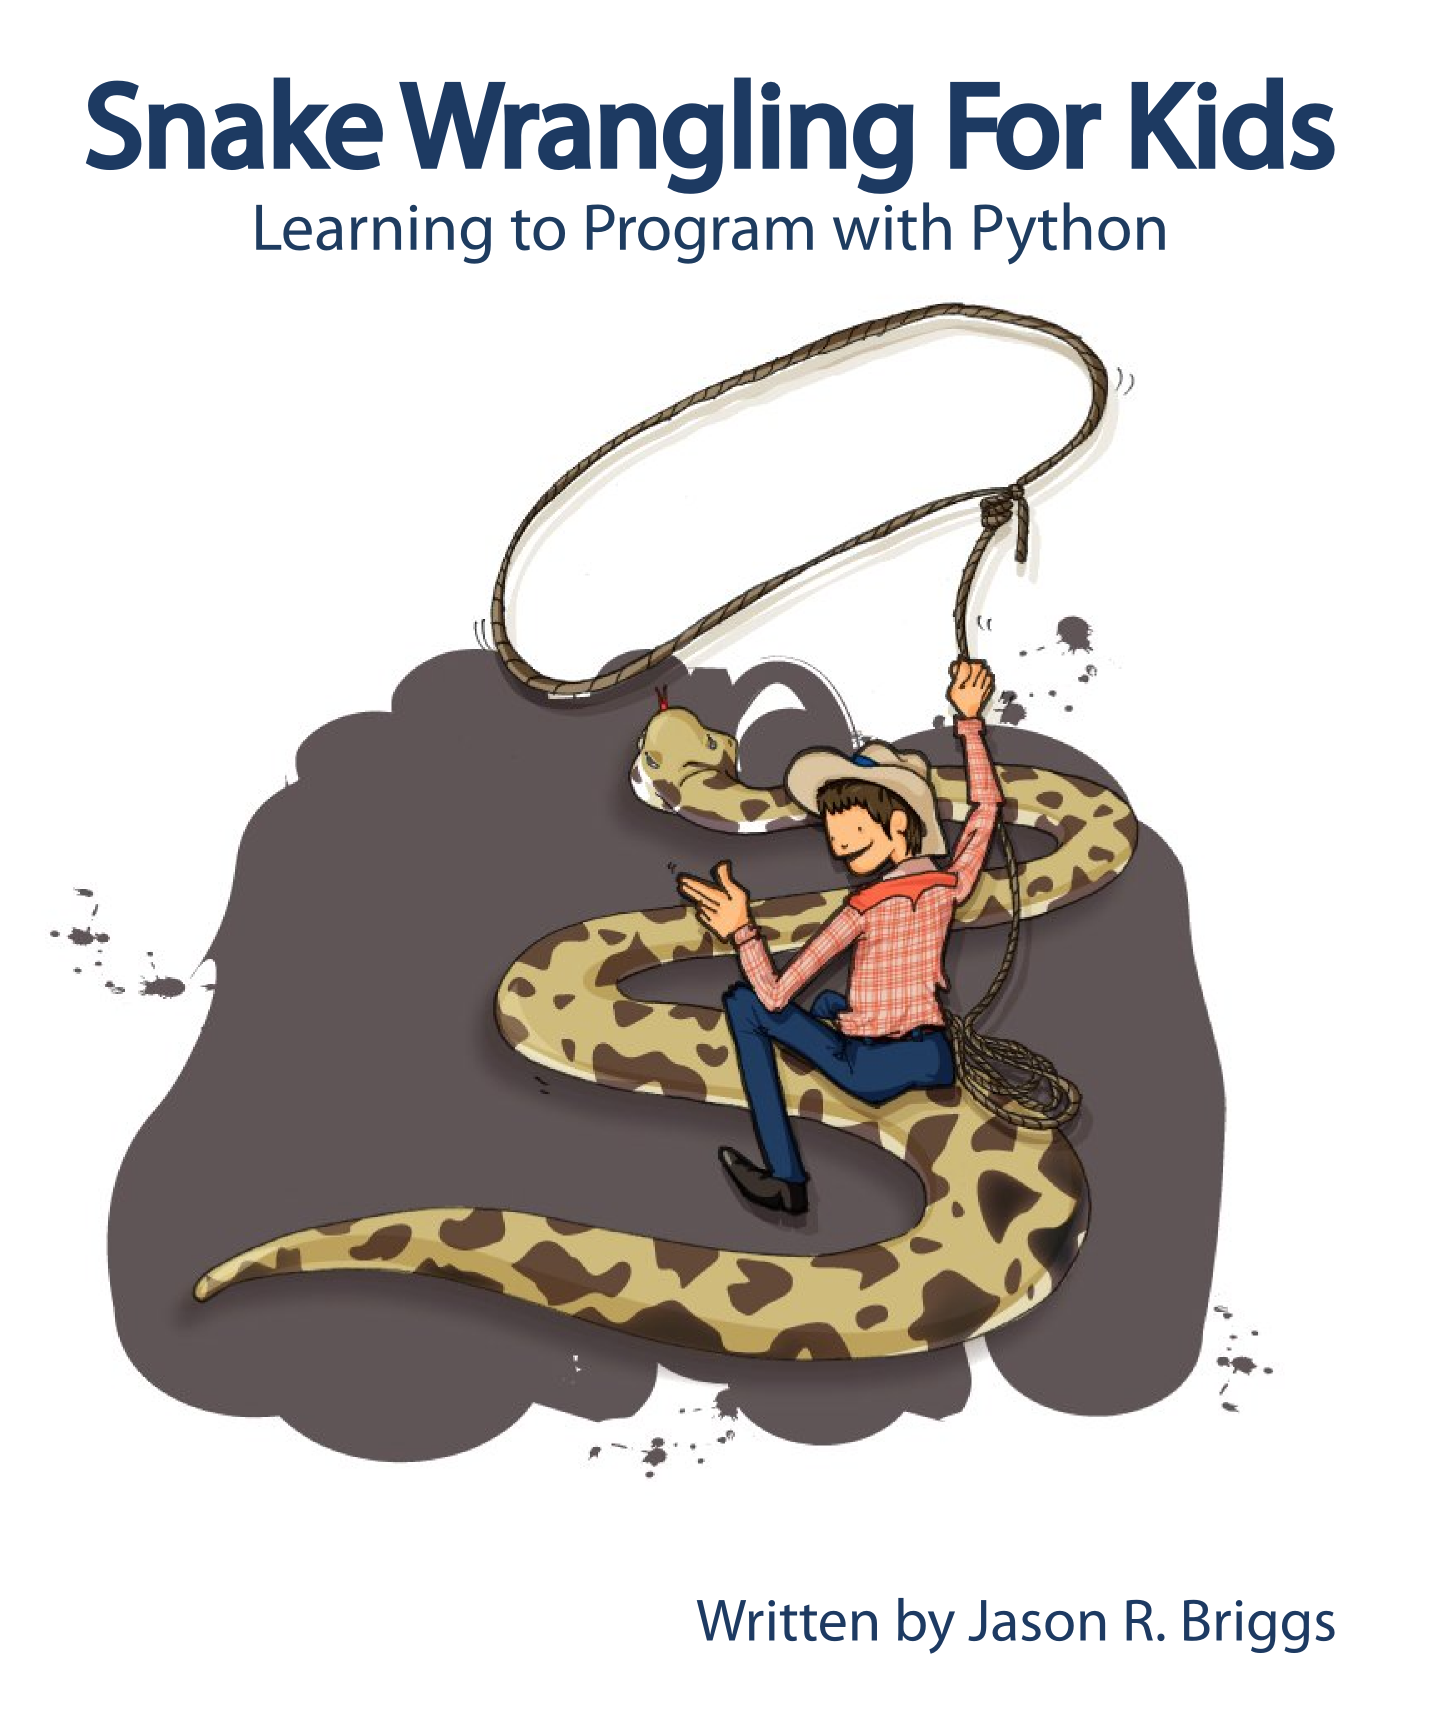
\includegraphics[width=0.9\paperwidth]{../en/cover.eps}
\end{textblock*}
\begin{flushright}
\vspace{30mm}
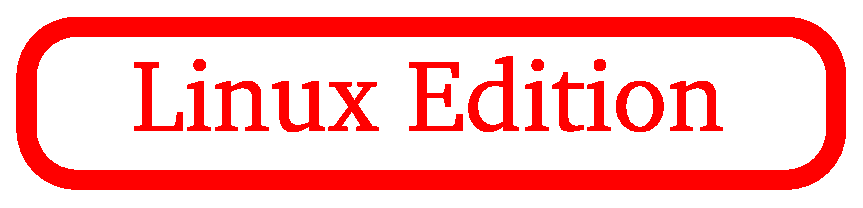
\includegraphics[width=40mm]{../en/linux-edition.eps} 
\end{flushright}
\end{titlepage}

\noindent
\textsf{\emph{Snake Wrangling for Kids, Learning to Program with Python}}\\
by Jason R. Briggs\\
перевод на русский:\\
Кочетов Е.\,М. <Egor.Kochetoff@gmail.com>\\
\\
Version 0.7.7
\\\\
Copyright \copyright 2007.\\
\\
Cover art and illustrations by Nuthapitol C.\\
\\
\noindent
\textsf{\emph{This book has been completely rewritten and updated, with new chapters (including developing graphical games), and new code examples. It also includes lots of fun programming puzzles to help cement the learning. Published by No Starch Press - available here: \href{http://nostarch.com/pythonforkids}{Python for Kids}. Also find more info \href{http://jasonrbriggs.com/python-for-kids/}{here}.}}
\\
\\
\linebreak
\noindent
Website:\\ \href{http://www.briggs.net.nz/log/writing/snake-wrangling-for-kids}{http://www.briggs.net.nz/log/writing/snake-wrangling-for-kids}\\ 
\\
\noindent
Thanks To:\\
Guido van Rossum (for benevolent dictatorship of the Python language), the members of the \href{http://www.python.org/community/sigs/current/edu-sig/}{Edu-Sig} mailing list (for helpful advice and commentary), author \href{http://www.davidbrin.com/}{David Brin} (the original \href{http://www.salon.com/tech/feature/2006/09/14/basic/}{instigator} of this book), Michel Weinachter (for providing better quality versions of the illustrations), and various people for providing feedback and errata, including: Paulo J. S. Silva, Tom Pohl, Janet Lathan, Martin Schimmels, and Mike Cariaso (among others).  Anyone left off this list, who shouldn't have been, is entirely due to premature senility on the part of the author.\\

\noindent
License:\\
\\

\includegraphics[width=40mm]{../en/by-nc-sa.eps}\\
This work is licensed under the Creative Commons Attribution-Noncommercial-Share Alike 3.0 New Zealand License. To view a copy of this license, visit\\ \href{http://creativecommons.org/licenses/by-nc-sa/3.0/nz/}{http://creativecommons.org/licenses/by-nc-sa/3.0/nz/} or send a letter to Creative Commons, 171 Second Street, Suite 300, San Francisco, California, 94105, USA.\\

\noindent
Below is a summary of the license.\\

\noindent
You are free:
\begin{itemize}
 \item \textbf{to Share} — to copy, distribute and transmit the work 
 \item \textbf{to Remix} — to adapt the work
\end{itemize}
\noindent
Under the following conditions:
\begin{description}
 \item[Attribution.] You must attribute the work in the manner specified by the author or licensor (but not in any way that suggests that they endorse you or your use of the work).
 \item[Noncommercial.] You may not use this work for commercial purposes.
 \item[Share Alike.] If you alter, transform, or build upon this work, you may distribute the resulting work only under the same or similar license to this one.
\end{description}

\noindent
For any reuse or distribution, you must make clear to others the license terms of this work.\\

\noindent
Any of the above conditions can be waived if you get permission from the copyright holder.\\

\noindent
Nothing in this license impairs or restricts the author's moral rights.\\

\vspace*{4cm}
\begin{center}

\includegraphics[width=5cm]{../en/python-powered.eps}
\end{center}

\mainmatter

\pagestyle{plain}

\pagenumbering{roman}
\tableofcontents
% preface.tex
% This work is licensed under the Creative Commons Attribution-Noncommercial-Share Alike 3.0 New Zealand License.
% To view a copy of this license, visit http://creativecommons.org/licenses/by-nc-sa/3.0/nz
% or send a letter to Creative Commons, 171 Second Street, Suite 300, San Francisco, California, 94105, USA.


\chapter*{Вступление}\normalsize
    \addcontentsline{toc}{chapter}{Вступление}
\begin{center}
{\em Пара слов для родителей...}
\end{center}
\pagestyle{plain}

Уважаемый родитель или иной управляющий компьютером!

Чтобы ваш ребёнок смог начать знакомиться с программированием, вам нужно установить Python на компьютер. Эта книга была недавно обновлена до версии Python 3.0, самой новой и несовместимой с предыдущими, так что если у вас установлена более старая версия Pyhton, вам стоит скачать и более старую версию этой книги.

Установка Python — достаточно простая задача, но есть несколько тонкостей — в зависимости от используемой операционной системы. Если вы только что купили сверкающий новый компьютер и не имеете никаких идей, что с ним делать, а предыдущее предложение начало вызывать у вас нервную дрожь или холодный пот, то, пожалуй, лучше вам найти кого-то кто сделает это за вас. Установка Python может занять от 15 минут до пары часов в зависимости от скорости интернета и компьютера.

Прежде всего, скачайте и установите последнюю версию Python 3 для вашего дистрибутива. Дистрибутивов очень много, так что инструкции для всех тут привести не получится… да и скорее всего, если вы используете Linux, то уже знаете, как это сделать. Наверное, вы даже возмущены самой идеей того чтобы рассказывать вам, как что-либо устанавливать, так что тут я остановлюсь.

\note{После установки…}

…Вам, возможно, придётся в течение первых пары глав посидеть с ребёнком рядом, но после нескольких примеров ему будет только приятнее читать книгу самому (с компьютером вместе). Нужно рассказать ребёнку, как вводить команды в консоль, как пользоваться текстовым редактором (наподобие блокнота; Microsoft Word никак не подойдёт), открывать и сохранять файлы в этом редакторе. Всё остальное расскажет эта книга.

\vspace{12pt}
\noindent
Спасибо за уделённое время; с наилучшими пожеланиями,\\
КНИГА.


\pagenumbering{arabic}
\pagestyle{headings}
% !TeX encoding = UTF-8
% Use XeLaTeX to compile it
%
% Эта работа распространяется на условиях лицензии Creative Commons Attribution-Noncommercial-Share Alike 3.0 New Zealand License.
% Краткое описание лицензии есть тут: http://creativecommons.org/licenses/by-nc-sa/3.0/nz/deed.ru
% Полное — там же.
% Эту книгу можно невозбранно распространять и изменять, но только соблюдая следующие условия:
% сохраняя лицензию и не вводя дополнительных ограничений, бесплатно
% и указывая авторство как оригинальной части, так и изменённой.
% Автор оригинального английского текста — Jason R Briggs http://jasonrbriggs.com/
% Автор перевода — Егор Кочетов <Egor.Kochetoff@gmail.com>
%
% This work is licensed under the Creative Commons Attribution-Noncommercial-Share Alike 3.0 New Zealand License.
% To view a copy of this license, visit http://creativecommons.org/licenses/by-nc-sa/3.0/nz
% or send a letter to Creative Commons, 171 Second Street, Suite 300, San Francisco, California, 94105, USA.
%

\chapter{Не все змеи будут шипеть на тебя}\label{ch:notallsnakeswillsquishyou}

Возможно, тебе подарили эту книгу на день рожденья. А может, на рождество. Например, так: тётя Агата (у всех есть тётя Агата, но не все об этом знают) хотела подарить носки, хотя и не парные, но оба красивые, на два размера больше — на вырост (и всё равно бы эти носки не пригодились потом). А потом вместо этого услышала про эту книгу (которую можно взять и напечатать), вспомнила твои вопросы про всякие компьютерные штуки, и твои непонятные объяснения, как пользоваться компьютером, оборвавшиеся в момент, когда она начала разговаривать с компьютерной мышью, и решила подарить эту книгу. Во всяком случае эта книга уж точно лучше пары разных носков.

Надеюсь, я не слишком тебя разочаровываю тем, что я — возможно, напечатанная на какой-нибудь старой обёрточной бумаге (хотя если повезло, то и нет) — не слишком разговорчивая (прямо, скажем, совсем молчаливая) книга, с пугающим словом «изучение» в названии... Но представь на минутку и мои ощущения. Если бы вот ты был персонажем из какой-нибудь книги про волшебников, одна из которых наверняка есть у тебя в спальне на книжной полке, — у меня бы могли быть зубы... или даже глаза! А ещё какие-нибудь движущиеся картинки, таинственные звуки... ладно, чего я. В общем, я просто бумажная книжка, хотя могло бы быть и лучше.

\btw{Ах, много бы я дала за пару хороших острых челюстей...}

Но вообще, быть конкретно такой книжкой тоже не слишком печально. Ну не могу я говорить... пальцы покусывать не могу; зато могу рассказать немного о том, что заставляет компьютеры работать. Не про разные аппаратные штуки — все эти провода, платы, чипы — они меня немного пугают. Электричеством, например, могут ударить (так что не стоит и пытаться туда лезть, как по мне). Я могу рассказать о том, что удивительным образом скрыто внутри всех этих проводов, микросхем и что делает компьютер по-настоящему полезным.

\begin{wrapfigure}{r}{0.5\textwidth}
  \begin{center}
\includegraphics*[width=70mm]{../en/electrocute.eps}
  \end{center}
\end{wrapfigure}

Вообще, это здорово похоже на мысли, например, в твоей голове. Если бы мыслей у тебя не было — сидел бы ты, скажем, на полу в спальне и бессмысленно смотрел в пространство перед собой. Без \emph{программ} компьютеры бы могли приносить пользу, пожалуй, разве что как стопор для двери. Да и то посредственный: вечно все бы об него спотыкались по ночам. А что может быть хуже, чем удариться ночью в темноте пальцем ноги с размаху о железный угол...

\btw{Итак, я всего лишь книга. И мне это хорошо известно.}

Вообще, у тебя в семье могут быть разные устройства вроде Playstation, Xbox, Wii — игровые консоли, — а ещё DVD-проигрыватель, может, даже современный холодильник и игрушечная машинка. В них во всех есть программы, которые делают их намного полезнее, чем если бы эти штуки были без программ. В DVD-проигрывателе есть программа для чтения и воспроизведения дисков. В холодильнике — какая-то простая программа для поддержания температуры при минимальных затратах электричества. В машинке — программа для приёма команд с пульта управления и для езды в ответ на эти команды. А в настоящих машинах программы показывают маршруты в объезд пробок и сигналят водителю, когда он паркуется, чтоб он никуда не въехал (в стену или соседнюю машину).

Зная, как писать программы, ты сможешь сделать множество самых разных полезных вещей. Можно свою игру написать. Можно писать страницы в интернете, которые что-нибудь делают, а не просто показывают текст и картинки. Можно упрощать себе выполнение домашней работы.

Так вот, пора приступить к чему-то чуть более интересному, чем эти рассуждения.

\section{Пара слов про язык}

Так же как и у людей, определённо как у китов, возможно, и у дельфинов и, возможно, у родителей (тут, конечно, спорно), у компьютеров есть свой собственный язык. Вообще, как и у людей, у компьютеров много языков. Какую букву английского алфавита ни возьми, она называет какой-нибудь язык. Вот, например, буквы A, B, C, D, E — не только буквы, но и названия языков программирования (что ещё раз доказывает, что у взрослых никакого воображения и хорошо бы им давать почитать хотя бы словарь перед тем, как названия придумывать).

Есть ещё языки программирования, названные в честь людей\footnote{например, язык Ада — в честь \href{https://ru.wikipedia.org/wiki/\%D0\%9B\%D0\%B0\%D0\%B2\%D0\%BB\%D0\%B5\%D0\%B9\%D1\%81,_\%D0\%90\%D0\%B4\%D0\%B0}{Ады Лавлейс}. А есть ещё язык \href{https://ru.wikipedia.org/wiki/\%D0\%A3\%D1\%87\%D0\%B5\%D0\%B1\%D0\%BD\%D1\%8B\%D0\%B9_\%D0\%B0\%D0\%BB\%D0\%B3\%D0\%BE\%D1\%80\%D0\%B8\%D1\%82\%D0\%BC\%D0\%B8\%D1\%87\%D0\%B5\%D1\%81\%D0\%BA\%D0\%B8\%D0\%B9_\%D1\%8F\%D0\%B7\%D1\%8B\%D0\%BA}{РАЯ}.},
есть языки-сокращения из заглавных букв (SQL, например),  есть немножко названных в честь телевизионных шоу. А, да, ещё если дописать к этим буквам всяких значков типа плюсиков, решёточек (+, \#), то тоже получатся названия разных языков программирования. И ещё впридачу некоторые языки очень похожи и отличаются только в каких-то мелочах.

\btw{Что я говорила? Никакого воображения!}

К счастью, многие из языков уже почти не используются или совсем исчезли; но однако же список способов «говорить» с компьютером всё ещё пугающе велик. Я буду обсуждать только один из них, потому что иначе всё так и закончится их перечислением, не успеем мы приступить к чему-то действительно интересному.

\section{Орден Неядовитых Удушающих Змей...}

... или просто питонов.

Вообще, питон — не только змея\footnote{которая \href{https://ru.wikipedia.org/w/index.php?title=\%D0\%9F\%D0\%B8\%D1\%82\%D0\%BE\%D0\%BD\%D1\%8B&oldid=70828612\#.D0.9F.D0.B8.D1.82.D0.B0.D0.BD.D0.B8.D0.B5}{может} не есть полтора года кряду!}, но и язык программирования. Многие называют его «пайтон», как принято за рубежом, где его и придумали (и пишут его название как Python). Язык, правда, был назван не в честь змеи — это один из немногих языков программирования, названных в честь телевизионного шоу. \href{http://www.youtube.com/watch?v=YO2xZbac7lw&list=PL89E217812DCA2BDA}{Монти Пайтон} (Monty Python) — \href{http://www.montypython.com/}{британское телешоу}, популярное с 1970х годов. Требуется достичь некоторого возраста и иметь определённый склад ума, чтобы счесть его забавным, но многим нравится. Хотя лет до 12 смотреть вообще смысла нет, будет скучно и непонятно.

Есть несколько особенностей Питона (языка программирования, а не змеи), делающих его очень полезным, чтобы учиться программировать. Для нас сейчас важнее всего то, что используя его, можно быстро сесть и начать писать какие-то программки, пусть и очень простые, без долгих разговоров и объяснений.

Это тот момент, когда надо убедиться, что твоя мама, папа или кто там управляет компьютером прочли часть «Заметка для мам и пап». Есть хороший способ проверить это. Спроси у них, как называется программа-\emph{эмулятор терминала} — это может быть \texttt{yakuake}, \texttt{konsole}, \texttt{rxvt}, \texttt{xterm} или ещё какая-нибудь, их очень много бывает — именно поэтому придётся спросить. Запусти эту программу, напиши \emph{в командной строке} «python3» (без кавычек) и нажми на клавиатуре клавишу Enter. На экране должно появиться что-то похожее на рисунок \ref{fig4}.

\begin{figure}
\begin{center}
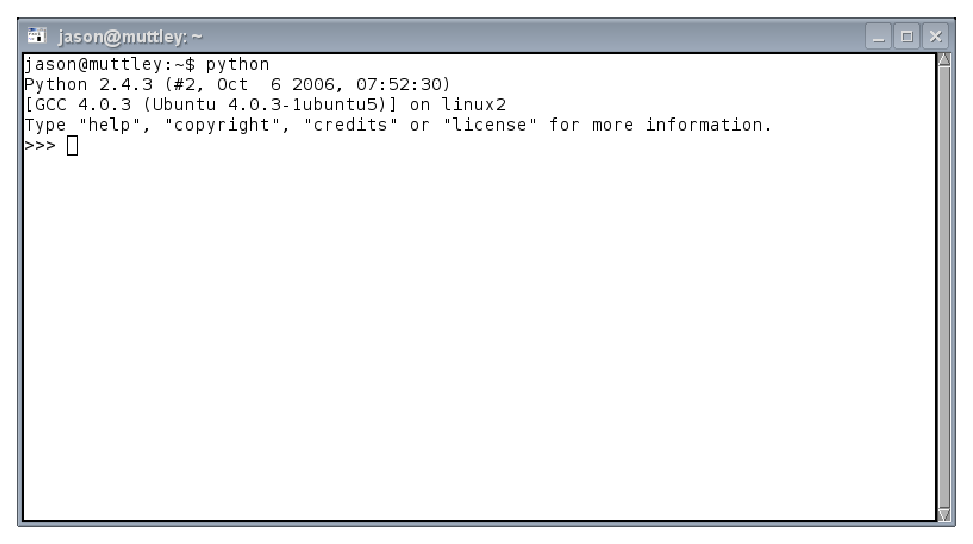
\includegraphics[width=80mm]{../en/figure4.eps}
\end{center}
\caption{Консоль Питона в Линуксе.}\label{fig4}
\end{figure}

\begin{samepage}
\note{Если ты обнаружишь, что они не прочитали инструкции в начале книги...}
\nopagebreak
\paragraph*{}
... и из-за этого у тебя не получилось что-то сделать, то перелистни эту книгу на начало, подсунь им под нос введение, пока они читают утреннюю газету, и умоляюще посмотри на них. Иногда помогает говорить «пожалуйста-пожалуйста-пожалуйста» до тех пор, пока они не встанут и не сделают всё, что надо. Ну и конечно, можно попробовать сделать всё самостоятельно, это может оказаться даже проще.
\end{samepage}

\section{Первая программа на Питоне}

Так или иначе, если ты добрался досюда, у тебя уже открыта \emph{консоль}, или командная строка Питона — это один из способов запускать команды и целые программы на Питоне. После запуска консоли или ввода любой команды ты увидишь \emph{приглашение командной строки}, которое в Питоне выглядит вот так:

\begin{verbatim}
>>>
\end{verbatim}

Если записать несколько команд на Питоне одну за другой, получится программа, которую можно запускать и не через консоль, но пока на минутку остановимся на простых командах, которые можно вводить прямиком в командную строку (после «приглашения»). Например, можно ввести туда следующую команду:

\begin{verbatim}
print("Всем привет!")
\end{verbatim}

Чтобы всё получилось, нужно ввести и скобки и кавычки (вот эти: "") так, как написано выше. Тогда на экране должно появиться что-то вроде такого:

\begin{verbatim}
>>> print("Всем привет!")
Всем привет!
\end{verbatim}

После этого приглашение командной строки появится снова, чтобы показать, что Питон готов принимать новые команды. Поздравляю! Ты только что создал и запустил свою первую программу на Питоне — пусть пока и всего из одной команды: print — функции, которая просто печатает всё, что написано в скобках. Потом мы много будет использовать эту команду.

\section{Вторая программа на питоне… опять то же самое?}

Программы на Питоне были бы не слишком полезными, если бы их приходилось каждый раз вводить заново в командную строку или если бы ты написал программу для кого-то, а ему бы пришлось её перепечатывать, чтобы запустить.

Программа для редактирования текстов (Microsoft Word, Libreoffice Writer или другая подобная), которую ты, вероятно, используешь для выполнения каких-нибудь домашних заданий, получена из исходного кода размером примерно от 10 до 100 миллионов строк. Если печатать это на бумаге с двух сторон не очень крупно, это может занять, например, 400 000 страниц. Это стопка бумаги высотой 40 метров, с десятиэтажный дом. Такое количество бумаги нести из магазина в дом, чтобы перепечатать, пришлось бы долго… очень долго…

…а если бы ещё и ветер подул в подходящий момент… за бумагой пришлось бы долго бегать. Так вот, хорошая новость: всем этим заниматься не обязательно.

\begin{center}
\includegraphics*[width=85mm]{../en/pullinghair.eps}
\end{center}

Открой текстовый редактор (можешь опять спросить у родителей, как он называется: например, kate, gedit, kdevelop, но никак не Microsoft Word, он не подойдёт) и напиши туда точно ту же самую команду, что ты до этого вводил в консоль:

\begin{verbatim}
print("Всем привет!")
\end{verbatim}

%todo save.png
Теперь сохрани этот файл в своей домашней папке. Наверху в программе должен быть значок сохранения, а когда тебя спросят, куда сохранять, нажми на какую-нибудь кнопку типа домика. В качестве имени файла введи «hello.py». Теперь опять открой терминал и напиши:

\begin{verbatim}
python hello.py
\end{verbatim}

В консоли должно появиться приветствие от программы, точно так же, как в прошлый раз (примерно как на рисунке \ref{fig9}).

\begin{figure}
\begin{center}
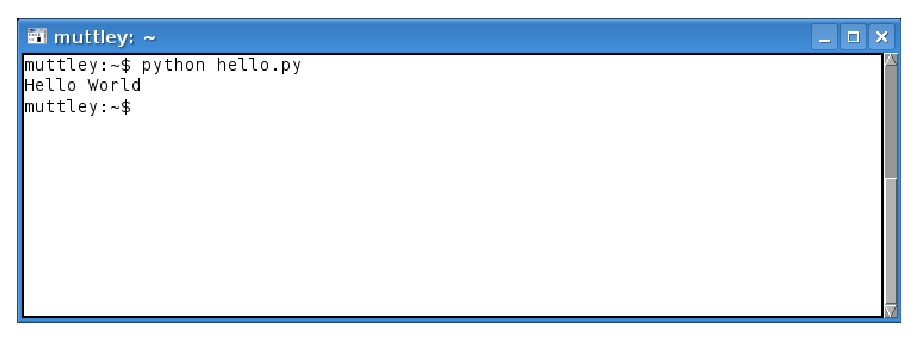
\includegraphics[width=75mm]{../en/figure9.eps}
\end{center}
\caption{Запуск программы на Питоне, сохранённой в текстовый файл}\label{fig9}
\end{figure}

Вот. Теперь ты видишь, что мудрые люди, создавшие Питон, спасли тебя от ввода одних и тех же программ много-много-много раз для выполнения одних и тех же действий. Как они делали в 1980х. Я серьёзно, им приходилось вводить каждый раз кучу команд для выполнения одной и той же программы. Можешь спросить у папы — вдруг у него был ZX81 в молодости — так там приходилось так делать. Теперь можно просто написать имя программы, и она целиком исполнится от начала до конца.

\note{Конец начала}

Добро пожаловать в удивительный мир программирования!
Мы начали с простой программы, которая печатает «Всем привет» («Hello world») — все с этого начинают, когда учатся программировать. В следующей главе мы займёмся чуть более полезными вещами в консоли Питона, а потом изучим, как написать программу посложнее.

% !TeX encoding = UTF-8
% Use XeLaTeX to compile it
%
% Эта работа распространяется на условиях лицензии Creative Commons Attribution-Noncommercial-Share Alike 3.0 New Zealand License.
% Краткое описание лицензии есть тут: http://creativecommons.org/licenses/by-nc-sa/3.0/nz/deed.ru
% Полное — там же.
% Эту книгу можно невозбранно распространять и изменять, но только соблюдая следующие условия:
% сохраняя лицензию и не вводя дополнительных ограничений, бесплатно
% и указывая авторство как оригинальной части, так и изменённой.
% Автор оригинального английского текста — Jason R Briggs http://jasonrbriggs.com/
% Автор перевода — Егор Кочетов <Egor.Kochetoff@gmail.com>
%
% This work is licensed under the Creative Commons Attribution-Noncommercial-Share Alike 3.0 New Zealand License.
% To view a copy of this license, visit http://creativecommons.org/licenses/by-nc-sa/3.0/nz
% or send a letter to Creative Commons, 171 Second Street, Suite 300, San Francisco, California, 94105, USA.
%

\chapter{8 умножить на 3.57 равняется…}\label{ch:8multipliedby3.57}

Чему равно 8 умножить на 3.57? Пришлось бы использовать калькулятор, чтобы посчитать? Ладно, этот пример можно вычислить и в уме, но не в том дело. То же самое можно сделать в консоли Питона. Запусти её опять (как описано в предыдущей главе), если она ещё не запущена, и введи туда такую команду: \texttt{8*3.57}. Потом нажми Enter.

\begin{verbatim}
Python 3.4.0 (default, Apr 11 2014, 13:05:11) 
[GCC 4.8.2] on linux
Type "help", "copyright", "credits" or "license" for more information.
>>> 8 * 3.57
28.56
\end{verbatim}

Звёздочка (\code{*}) (обычно это shift + 8) используется для умножения\index{умножение} вместо привычного символа $×$ (или $\cdot$), потому что не везде их можно просто так ввести с клавиатуры, а буква X путалась бы с собственно буквой, если бы её использовали как знак умножения. Ладно, как насчёт чего-нибудь более полезного?

Представь, что тебе приходится заниматься делами по хозяйству раз в неделю, за что каждый раз ты получаешь по 5 рублей и ещё у тебя есть курьерская подработка по доставке газет за 30 рублей в неделю. Сколько денег такими темпами накопится за год?

\begin{figure}[t]
\begin{center}
\fbox{\colorbox{PaleBlue}{\parbox{.75\linewidth} {
\subsection*{Питон сломался!?!?}

Если ты возьмёшь калькулятор и введёшь туда \texttt{8×3.57}, ответ на экране будет такой:

\vspace{10pt}
\textsf{28.56}
\vspace{10pt}

В Питоне ответ может быть такой же, а может быть такой:

\vspace{10pt}
\textsf{28.55999999}
\vspace{10pt}

Чем Питон отличается? Уж не поломан ли он??

Да нет, вообще-то. Просто так дробные числа (числа с десятичной запятой, или \emph{числа с плавающей запятой}\index{числа с плавающей запятой}) представляются в компьютере: приближённо. Результаты всегда почти точные, но далеко справа после точки могут набегать небольшие ошибки вычисления после выполнения последовательности действий. Дробные числа представляются в компьютере не очень просто, мы не будем сейчас на этом останавливаться. Я хочу сказать, не удивляйся, что \emph{иногда} результаты вычислений не в точности равны тому, что ты ожидаешь; это верно для умножения, деления, сложения и вычитания.

Целые числа в компьютере представляются точно и всегда вычисляются без ошибок в Питоне (в других языках программирования есть свои хитрости).
}}}
\end{center}
\end{figure}

Если бы мы решали эту задачу на бумаге, то написали бы что-то вроде:

\begin{verbatim}
(5 + 30) × 52
\end{verbatim}

Что значит: (5 руб + 30 руб), умноженное на 52 недели в году.
\begin{samepage}
Можно, конечно, и сразу сократить эту запись до такой:

\begin{verbatim}
35 × 52
\end{verbatim}
\end{samepage}

И это уже совсем просто посчитать что на калькуляторе, что в столбик (в уме сложнее). А можно всё то же самое сделать в консоли:

\begin{listing}
\begin{verbatim}
>>> (5 + 30) * 52
1820
>>> 35 * 52
1820
\end{verbatim}
\end{listing}

Как быть, если ты тратишь 10 рублей в неделю? Что теперь останется к концу года? Можно было бы разными способами записать это на бумаге, но давай опять обратимся к консоли:

\begin{listing}
\begin{verbatim}
>>> (5 + 30 - 10) * 52
1300
\end{verbatim}
\end{listing}

Это значит: 5 рублей и ещё 30 рублей минус 10 потраченных рублей, и всё умножается на 52 недели в году. В конце года будет 1300 накопленных рублей. Ладно, я понимаю, что выглядит это всё не слишком полезно, и без Питона тут было бы легко обойтись. Мы потом опять вспомним про этот пример, и я покажу, как сделать из него куда более полезный.

В питоньей консоли можно умножать\index{умножение}, складывать\index{сложение}, вычитать\index{вычитание} и делить\index{деление}. Можно выполнять и другие арифметические действия, но мы пока их пропустим. Вот так выглядят символы математических операций\index{математические операции}:

\begin{center}
\begin{tabular}{|c|c|}
\hline
$+$ & Сложение \\
\hline
$-$ & Вычитание \\
\hline
$*$ & Умножение \\
\hline
$/$ & Деление \\
\hline
\end{tabular}
\end{center}

Для деления используется косая черта («прямой слэш» или просто «слэш», как его ещё называют), потому что рисовать дроби с клавиатуры не так-то просто, а символа деления ($\div$) обычно тоже нет.

Если бы тебя попросили сказать, сколько коробок, в которые влезает по 20 яиц, нужно для 100 яиц, ты мог бы написать что-то такое:

\begin{displaymath}
\frac{100}{20}
\end{displaymath}

или такое:

\begin{displaymath}
\begin{array}{rr|r}
100&&20\\
\cline{3-3}
100&&5\\
\cline{1-1}
0
\end{array}
\end{displaymath}

ну или, может, такое (хотя так чаще за рубежом пишут)

\begin{displaymath}
100 \div 20
\end{displaymath}

Так вот, в Питоне надо написать вот так: \code{100 / 20}.

\btw{Что, на мой взгляд, гораздо проще. Впрочем, что я в этом понимаю, я всего лишь книга.}

\section{Использование скобок и «приоритет операций»}\index{приоритет операций}

В языках программирования (да и просто в математике) мы используем скобки, чтобы управлять тем, что называется «приоритет операций». Операции не ограничиваются четырьмя арифметическими, бывают и другие, но смысл одинаковый. Из этих четырёх операций умножение и деление, как обычно, выполняются перед сложением и вычитанием, то есть у них выше приоритет. В примере ниже у всех операций одинаковый приоритет, поэтому они все выполняются слева направо:

\begin{listing}
\begin{verbatim}
>>> print(5 + 30 + 20)
55
\end{verbatim}
\end{listing}

В примере ниже тоже у всех одинаковый приоритет, и тоже все операции выполняются по порядку слева направо:

\begin{listing}
\begin{verbatim}
>>> print(5 + 30 - 20)
15
\end{verbatim}
\end{listing}

А вот в следующем примере есть умножение. Тут сначала умножаются числа 20 и 30, а потом к ним прибавляется 5: у умножения выше приоритет.

\begin{listing}
\begin{verbatim}
>>> print(5 + 30 * 20)
605
\end{verbatim}
\end{listing}

Что будет, если добавить скобок? Вот что:

\begin{listing}
\begin{verbatim}
>>> print((5 + 30) * 20)
700
\end{verbatim}
\end{listing}

Почему поменялся результат? Потому что скобки меняют порядок операций. Сначала вычисляется то, что в скобках, а потом всё, что снаружи. Тут сначала к 5 прибавляется 30, а результат всего Питон умножает на 20.

Можно использовать скобки более сложным образом. Можно внутри скобок писать ещё скобки:

\begin{listing}
\begin{verbatim}
>>> print(((5 + 30) * 20) / 10)
70
\end{verbatim}
\end{listing}

Тут Питон сначала вычисляет то, что внутри самых вложенных скобок, потом то, что во внешних скобках, и потом выполняет операцию деления, которая вообще не в скобках (самые внешние скобки нужны слову print, а не чтобы указывать порядок операций). Это выражение можно прочитать так: «прибавь к 5 30, потом это всё умножь на 20 и результат подели на 10». Без скобок всё было бы иначе:

\begin{listing}
\begin{verbatim}
>>> 5 + 30 * 20 / 10
65
\end{verbatim}
\end{listing}

Тут сначала 30 умножается на 20, потом делится на 10 и к этому всему прибавляется 5.

\btw{Помни, что умножение и деление всегда выполняются перед сложением и вычитанием, если только скобки не указывают делать иначе.}

\section{Нет ничего столь же непостоянного, как переменная}\index{переменные}

«Переменная» в программировании — название места для хранения разных штук. «Разные штуки» могут быть числами, текстом, списками чисел или строк и множеством других вещей, о которых обо всех сейчас пока рассказать сложно. Давай пока считать, что переменная — это что-то вроде почтового ящика.

\begin{center}
\includegraphics*[width=76mm]{../en/girlbubble.eps}
\end{center}

В почтовый ящик можно положить что-нибудь: письмо, газету — и в переменную можно точно так же положить что-нибудь: число, строку, список чисел. Именно таким образом работают переменные в большинстве языков программирования: в них что-нибудь кладут. Правда, не во всех языках так.

В Питоне переменные используются немножко иначе. Они не хранят что-то внутри себя, а, скорее, работают наклейкой на почтовом ящике. Эту наклейку можно снять и переклеить на другой ящик, например. А можно прилепить сразу на несколько каких-нибудь коробок (обмотав их предварительно скотчем). В питоне эта операция прилепливания выглядит как знак равенства. Чтобы создать переменную, нужно написать её имя слева от этого знака, а справа — то, на что эта переменная указывает. Например, вот так:

\begin{listing}
\begin{verbatim}
>>> Фёдор = 100
\end{verbatim}
\end{listing}

Мы сейчас создали переменную, называющуюся \code{Фёдор}, и сказали, что она указывает на число 100. Тут мы ещё говорим Питону запомнить это число, потому что собираемся его потом использовать. Чтобы узнать, на что переменная указывает, можно вывести её значение функцией \code{print}, как-то так:

\begin{listing}
\begin{verbatim}
>>> Фёдор = 100
>>> print(Фёдор)
100
\end{verbatim}
\end{listing}

Можно сказать Питону, что \code{Фёдор} теперь должен указывать на другое число:

\begin{listing}
\begin{verbatim}
>>> Фёдор = 200
>>> print(Фёдор)
200
\end{verbatim}
\end{listing}

%TODO уточнить процент лабуды в следующем предложении. Константы реально сборщиком мусора убираются в питоне?
Теперь \code{Фёдор} указывает на число 200 (а число 100, которое больше не нужно, Питон потом забудет, когда оно будет мешать). И \code{print} подтвердил нам, что Фёдор теперь указывает на 200.
Можно наклеить на это же самое 200 и ещё одну наклейку, то есть создать ещё одну переменную, указывающую на него:

\begin{listing}
\begin{verbatim}
>>> Фёдор = 200
>>> Василий = Фёдор
>>> print(Василий)
200
\end{verbatim}
\end{listing}

В этом кусочке кода мы создаём переменную \code{Василий}, которая указывает туда же, куда и \code{Фёдор}. Если Фёдор поменяет своё значение, Василия это не коснётся.

Вообще, конечно, «Фёдор» — не самое подходящее имя для переменной. Обычно имена переменных записывают английскими буквами — так программистам со всего мира гораздо проще читать и дополнять программы друг друга. Ну и кроме того, имя переменной должно бы говорить, зачем она нужна. Вот с почтовым ящиком всё понятно, он нужен, чтобы разную почту хранить. А переменная может хранить совершенно разные вещи, совсем по-разному устроенные, и переменных в программе обычно очень много. Поэтому называть переменную нужно так, чтобы сразу было понятно, для чего она используется\footnote{Некоторые даже считают, что придумывать хорошие имена переменным — самое сложное в работе программиста.}.

Представь себе, что ты открыл консоль Питона, напечатал \code{Фёдор = 200}, а потом отошёл от компьютера. На 10 лет. Чтобы залезть на Эверест, потом пересечь пустыню Сахару, попрыгать с моста на резинке в Новой Зеландии и спуститься на лодках по реке Амазонке. И потом обратно вернулся к консоли. Самое сложное будет понять: почему Фёдор и почему 200?!

Обычно, чтобы всё забыть, хватает гораздо меньшего времени, чем 10 лет. А часто программу пишут сразу несколько людей, каждый из которых не знает мысли остальных. Так что лучше с самого начала называть все переменные понятно и не рассчитывать на свою память.

Так-то! Смотри, например, мы можем назвать переменную так:\\\code{number\_of\_students}.

\begin{listing}
\begin{verbatim}
>>> number_of_students = 200
\end{verbatim}
\end{listing}

Так сделать получится, потому что имена переменных можно составлять из букв, цифр и знаков подчёркивания (главное, чтобы имя не начиналось с цифры). Если ты вернёшься к своему коду через 10 лет, то «number\_of\_students» всё ещё будет иметь смысл (по крайней мере, если ты знаешь английский хоть немного, что в любом случае пригодится). Можно будет напечатать вот так:

\begin{listing}
\begin{verbatim}
>>> print(number_of_students)
200
\end{verbatim}
\end{listing}

И сразу будет понятно, что количество студентов (где-то) — 200. Не всегда есть смысл придумывать длинные осмысленные имена переменных: иногда переменная используется всего в паре строк, иногда можно использовать вообще одну букву в качестве имени, и есть такие случаи, когда всем это будет привычно и понятно. В основном, это зависит от того, захочется ли потом понять по имени переменной, зачем она вообще нужна, или это будет почему-нибудь понятно и без этого.

\begin{listing}
\begin{verbatim}
это_тоже_допустимое_имя_переменной_но_наверное_не_слишком_полезное
\end{verbatim}
\end{listing}

\section{Используем переменные}\index{переменные}

Ладно, как создавать переменные мы разобрались. Но что с ними делать?

А вот что. Помнишь тот пример, который мы считали выше? Сколько денег заработается за год? Вот этот:

\begin{listing}
\begin{verbatim}
>>> print((5 + 30 - 10) * 52)
1300
\end{verbatim}
\end{listing}

Что если нам сюда добавить три переменных? Вот так:

\begin{listing}
\begin{verbatim}
>>> chores = 5
>>> paper_round = 30
>>> spending = 10
\end{verbatim}
\end{listing}

В переменных записано, сколько денег получается за неделю: 5 руб. за домашние дела и 30 — за курьерство — и сколько денег тратится в неделю: 10 рублей. Можно теперь перепечатать тот же пример вот так:

\begin{listing}
\begin{verbatim}
>>> print((chores + paper_round - spending) * 52)
1300
\end{verbatim}
\end{listing}

Ответ такой же. А что если теперь за домашние дела ты будешь получать семь рублей вместо пяти? Надо записать в переменную \code{chores} значение 7, а потом нажать пару раз кнопку вверх на клавиатуре, чтобы появился опять пример на экране, и Enter, вот так:

\begin{listing}
\begin{verbatim}
>>> chores = 7
>>> print((chores + paper_round - spending) * 52)
1404
\end{verbatim}
\end{listing}

Так пришлось гораздо меньше печатать, чтобы получить новый ответ, чем без использования переменных. Можно попробовать поменять другие переменные и опять нажимать клавишу вверх, чтобы получать новые ответы:

\begin{listing}
\begin{verbatim}
Что будет если тратить вдвое больше:
>>> spending = 20
>>> print((chores + paper_round - spending) * 52)
884
\end{verbatim}
\end{listing}

Если тратить 20 рублей в неделю, то к концу года получится накопить только 884 рубля. Пока переменные не сильно много пользы нам принесли, но уже понятно, что с ними проще и что они могут что-нибудь хранить.

\btw{Вспоминай почтовый ящик с наклейкой на нём!}

\section{Кусочек строки}\index{строки}

Если ты уделяешь внимание моим словам, а не просто бегло проглядываешь книжку в поисках интересных картинок, то можешь вспомнить, что я говорила, что в переменных можно хранить разного сорта вещи, а не только числа. Например, можно хранить текст, или, как его обычно называют в программировании, строки (по-английски: \emph{string}). Такое название может поначалу показаться странным, но, если подумать, текст — это просто буквы, составленные в слова, составленные в строки, и ничего больше. Может быть, так понятнее.

\btw{А может, и не понятнее...}

В таком случае, всё, что тебе необходимо знать, — это что строка — не более чем составленные вместе буквы, цифры и любые другие символы. Ну и обычно они что-то значат все вместе. Всё содержимое этой книги можно записать в строку. Твоё имя можно записать строкой. Твой домашний адрес тоже. Мы, кстати, уже использовали строку в первой программе, вот эту: "Всем привет!".

В Питоне строка создаётся просто: нужно поставить кавычки (такие: " или такие: ') вокруг текста. Можно вспомнить про нашу бесполезную переменную Фёдора и записать в неё строку, вот так:

\begin{listing}
\begin{verbatim}
>>> Фёдор = "я маленькая строка"
\end{verbatim}
\end{listing}

И как всегда, можно узнать, что хранит Фёдор:

\begin{listing}
\begin{verbatim}
>>> print(Фёдор)
я маленькая строка
\end{verbatim}
\end{listing}

Или вот пример с одинарными кавычками:

\begin{listing}
\begin{verbatim}
>>> Фёдор = 'и я строка'
>>> print(Фёдор)
и я строка
\end{verbatim}
\end{listing}

\index{многострочная строка}Но если ты попытаешься сохранить в переменную сразу несколько строк текста\footnote{По-английски это называется \emph{multilne string}, то есть «многострочная строка». Строка с переносами строк внутри, иначе говоря.}, используя просто кавычки, то ничего не выйдет. Например, попробуй напечатать команду, написанную ниже, и получишь пугающе непонятное сообщение об ошибке, что-то вроде такого:

\begin{listing}
\begin{verbatim}
>>> Фёдор = "первая строка
  File "<stdin>", line 1
    Фёдор = "первая строка
                          ^
SyntaxError: EOL while scanning string literal
\end{verbatim}
\end{listing}

Про эту ошибку мы поговорим позже, а пока можешь просто запомнить, что чтобы сохранить в переменную сразу несколько строк текста, нужно использовать три одинарных кавычки\footnote{Обычно одинарную кавычку можно ввести только в английской раскладке и она находится на той же клавише, где русская «Э», справа→ на клавиатуре.}:

\begin{listing}
\begin{verbatim}
>>> Фёдор = '''вот строка
... с переносом строки внутри'''
\end{verbatim}
\end{listing}

Напечатай эту переменную, чтобы проверить, что всё получилось:

\begin{listing}
\begin{verbatim}
>>> print (Фёдор)
вот строка
с переносом строки внутри
\end{verbatim}
\end{listing}

Пока ты печатал эту строчку с переносом, то мог обратить внимание, что Питон вместо приглашения на второй строке напечатал три точки (...). Он это делает в тех случаях, когда что-то, начатое на первой строке, продолжается на следующей — вот как строка. Пока кавычки не закроются, Питон так и будет печатать «...», показывая, что ждёт завершения строки. Потом мы и в других случаях увидим эти три точки.

\section{Развлечения со строками}

Вот есть интересный вопрос: чему равно 10 * 5 (10 умножить на 5)? Ответ, конечно: 50.

\btw{Ладно, это был неинтересный вопрос.}

А чему равно 10 * 'а' (10 умножить на букву а)? Вопрос может показаться бессмысленным, но вот ответ от Питона:

\begin{listing}
\begin{verbatim}
>>> print(10 * 'a')
aaaaaaaaaa
\end{verbatim}
\end{listing}

Это работает не только с отдельными символами, но и со строками подлиннее:

\begin{listing}
\begin{verbatim}
>>> print(20 * 'abcd')
abcdabcdabcdabcdabcdabcdabcdabcdabcdabcdabcdabcdabcdabcdabcdabcdabcdabcdabcdabcd
\end{verbatim}
\end{listing}

Есть ещё один трюк со строками. В них можно вставлять значения. Для этого в строку нужно добавить «\%s» как маркер, куда вставлять значение. Проще всего это показать на примере:

\begin{listing}
\begin{verbatim}
>>> mytext = 'Мне %s лет'
>>> print(mytext % 12)
Мне 12 лет
\end{verbatim}
\end{listing}

%todo уточнить перевод placeholder
В первой строке создаётся переменная \code{mytext}, содержащая некоторые слова и шаблон подстановки (в английских инструкциях он называется \emph{placeholder}) \code{\%s}. Этот шаблон — это такая инструкция Питону: «замени меня чем-нибудь». На следующей строке, когда мы печатаем значение переменной \code{mytext}, мы используем символ \code{\%}, чтобы указать Питону, на что именно заменять шаблон подстановки: на число 12. Можно использовать одну и ту же строку и подставлять внутрь неё разные значения:

\begin{listing}
\begin{verbatim}
>>> mytext = 'Привет, %s, как твои дела?'
>>> name1 = 'Иннокентий'
>>> name2 = 'Саша'
>>> print(mytext % name1)
Привет, Иннокентий, как твои дела?
>>> print(mytext % name2)
Привет, Саша, как твои дела?
\end{verbatim}
\end{listing}

В примере выше создаются три переменных (\code{mytext}, \code{name1} и \code{name2}), первая из которых содержит маркер «\code{\%s}». Потом мы печатаем значение этой строки, подставляя внуть неё значения строк \code{name1} и \code{name2}, используя операцию «\code{\%}».

Можно вставить в строку больше, чем один шаблон для подстановки, вот так:

\begin{listing}
\begin{verbatim}
>>> mytext = 'Привет, %s и %s, как обстоят ваши дела?'
>>> print(mytext % (name1, name2))
Привет, Иннокентий и Саша, как обстоят ваши дела?
\end{verbatim}
\end{listing}

Когда используется несколько маркеров, нужно подставляемые переменные окружать скобками, как в примере выше. Несколько переменных, окружённых скобками, называются \emph{кортеж} (по английски — \emph{tuple}). Это слово потом ещё будет использоваться.

\section{Не совсем список для покупок}\index{списки}

Яйца, молоко, мыр, сельдерей, масло и сода. Не вполне полный список для покупок, но сойдёт для наших целей. Если бы тебе захотелось сохранить это в переменной, можно было бы это сделать так, в строку:

\begin{listing}
\begin{verbatim}
>>> shopping_list = 'яйца, молоко, сыр, сельдерей, масло, сода'
>>> print(shopping_list)
яйца, молоко, сыр, сельдерей, масло, сода
\end{verbatim}
\end{listing}

Другой способ — создать «список», особый сорт объектов в Питоне:

\begin{listing}
\begin{verbatim}
>>> shopping_list = [ 'яйца', 'молоко', 'сыр', 'сельдерей', 'масло', 'сода' ]
>>> print(shopping_list)
[ 'яйца', 'молоко', 'сыр', 'сельдерей', 'масло', 'сода' ]
\end{verbatim}
\end{listing}

Чтобы сделать список, приходится больше печатать (все эти кавычки), но результат сильно полезнее строки. Например, мы можем просто напечатать третий элемент списка, указав его \emph{индекс в списке} (позицию) в квадратных скобках:

\begin{listing}
\begin{verbatim}
>>> print(shopping_list[2])
сыр
\end{verbatim}
\end{listing}

Да, здесь нет опечатки. Мы напечатали третий элемент, хотя в квадратных скобках стоит цифра 2. Всё потому, что номера элементов в списке считаются с нуля. Это достаточно непривычно и кажется бессмысленным большинству людей — но не программистам\footnote{Индекс элемента в списке просто показывает, сколько элементов надо пропустить от начала списка, чтобы добраться до нужного. Индекс 0 значит, что пропускать не надо ни одного, индекс 2 — что надо пропустить 2 элемента, и получить как раз третий.}. Скоро ты тоже привыкнешь считать с нуля вместо одного, чем тоже будешь удивлять многих людей.

Можно ещё напечатать все элементы с третьего по пятый, используя двоеточие внутри квадратных скобок:

\begin{listing}
\begin{verbatim}
>>> print(shopping_list[2:5])
['сыр', 'сельдерей', 'масло']
\end{verbatim}
\end{listing}

\code{[2:5]} — значит: нужны все элементы с индексами от 2 до 5 (не включая 5). Поскольку индексы считаются с нуля, то получатся как раз третий, четвёртый и пятый элементы, а шестой (который с индексом 5) не будет включён в результат.

В списках можно хранить (как и в переменных) что угодно. Можно хранить числа:

\begin{listing}
\begin{verbatim}
>>> mylist = [ 1, 2, 5, 10, 20 ]
\end{verbatim}
\end{listing}

…и строки:

\begin{listing}
\begin{verbatim}
>>> mylist = [ 'a', 'bbb', 'ccccccc', 'ddddddddd' ]
\end{verbatim}
\end{listing}

…и всё вместе:

\begin{listing}
\begin{verbatim}
>>> mylist = [1, 2, 'a', 'bbb']
>>> print(mylist)
[1, 2, 'a', 'bbb']
\end{verbatim}
\end{listing}

…и другие списки:

\begin{listing}
\begin{verbatim}
>>> list1 = [ 'a', 'b', 'c' ]
>>> list2 = [ 1, 2, 3 ]
>>> mylist = [ list1, list2 ]
>>> print(mylist)
[['a', 'b', 'c'], [1, 2, 3]]
\end{verbatim}
\end{listing}

В примере выше создаётся перменная \code{list1}, содержащая список из трёх букв, и \code{list2}, содержащая список из трёх цифр; а потом создаётся переменная \code{mylist}, которая содержит оба эти списка. Дальше можно сходить с ума, создавая списки списков списков списков… но обычно никому не нужно делать такие сложные вещи в Питоне. С другой стороны, полезно знать, что так вообще можно и что список может хранить всё что угодно.

\btw{А не только какие продукты надо купить.}

\subsection*{\color{BrickRed}Изменяем элементы}\index{списки!изменение элементов}

Можно изменить элемент списка, просто присвоив ему новое значение, как будто это обычная переменная. Можно, например, заменить сельдерей салатом:

\begin{listing}
\begin{verbatim}
>>> shopping_list[3] = 'салат'
>>> print(shopping_list)
['яйца', 'молоко', 'сыр', 'салат', 'масло', 'сода']
\end{verbatim}
\end{listing}

\subsection*{\color{BrickRed}Добавляем ещё элементы...}\index{список!добавление элементов}

Можно добавить к списку новых элементов, вызвав функцию \code{append}. Подробно про функции (и как делать свои) мы поговорим позже, но пока можно воспользоваться готовой вот так:

\begin{listing}
\begin{verbatim}
>>> shopping_list.append('шоколадка')
>>> print(shopping_list)
['яйца', 'молоко', 'сыр', 'салат', 'масло', 'сода', 'шоколадка']
\end{verbatim}
\end{listing}

\btw{И этот список, несомненно, гораздо лучше оригинального.}

\subsection*{\color{BrickRed}$\ldots$и удаляем элементы}\index{списки!удаление}

Можно удалить из списка элементы, используя функцию \code{remove}. Например, чтобы удалить соду из списка, надо написать вот так:

\begin{listing}
\begin{verbatim}
>>> shopping_list.remove ('сода')
>>> print shopping_list
['яйца', 'молоко', 'сыр', 'салат', 'масло', 'шоколадка']
\end{verbatim}
\end{listing}

Ещё можно удалить элемент списка по ему индексу (как, кстати, и любую другую переменную). Для этого есть команда \code{del} (сокращение от слова \code{delete}, удалить), которая используется вот как:

\begin{listing}
\begin{verbatim}
>>> del shopping_list[0]
>>> print(shopping_list)
['молоко', 'сыр', 'салат', 'масло', 'шоколадка']
\end{verbatim}
\end{listing}

Теперь из списка исчез первый элемент — тот, который с индексом 0.

\subsection*{\color{BrickRed}Два списка лучше одного!}\index{списки!объединение}

Можно объединить два списка, сложив их, как будто мы складываем числа:

\begin{listing}
\begin{verbatim}
>>> list1 = [ 1, 2, 3 ]
>>> list2 = [ 4, 5, 6 ]
>>> print(list1 + list2)
[1, 2, 3, 4, 5, 6]
\end{verbatim}
\end{listing}

Можно записать результат сложения списков в новую переменную:

\begin{listing}
\begin{verbatim}
>>> list1 = [ 1, 2, 3 ]
>>> list2 = [ 4, 5, 6 ]
>>> list3 = list1 + list2
>>> print(list3)
[1, 2, 3, 4, 5, 6]
\end{verbatim}
\end{listing}

Кстати, этот метод можно использовать, чтобы добавлять в список новые значения вместо использования функции \code{append}. Вот, например, так:

\begin{listing}
\begin{verbatim}
>>> list1 = [ 1, 2, 3 ]
>>> list1 = list1 + [ 4 ]
>>> print (list1)
[1, 2, 3, 4]
>>> list1 = list1 + [5, 6, 7]
>>> print (list1)
[1, 2, 3, 4, 5, 6, 7]
\end{verbatim}
\end{listing}

Ещё список можно умножать примерно так же, как мы до этого умножали строку:

\begin{listing}
\begin{verbatim}
>>> list1 = [ 1, 2 ]
>>> print(list1 * 5)
[1, 2, 1, 2, 1, 2, 1, 2, 1, 2]
\end{verbatim}
\end{listing}

В примере выше умножение списка на 5 — это инструкция Питону «повтори список 5 раз.

Деление и вычитание для списка не имеют смысла, поэтому если попытаться так сделать, получится только ошибка:

\begin{listing}
\begin{verbatim}
>>> list1 / 20
Traceback (most recent call last):
  File "<stdin>", line 1, in <module>
TypeError: unsupported operand type(s) for /: 'list' and 'int'
\end{verbatim}
\end{listing}

или вот:

\begin{listing}
\begin{verbatim}
>>> list1 - 20
Traceback (most recent call last):
  File "<stdin>", line 1, in <module>
TypeError: unsupported operand type(s) for -: 'type' and 'int'
\end{verbatim}
\end{listing}

\btw{И попробуй угадай, что Питон хочет сказать этими сообщениями об ошибке…}

\section{Кортежи и списки}\label{tuplesandlists}\index{кортежи}

Кортеж (про который мы говорили раньше) вроде как список, но чтобы сделать его, нужно использовать круглые скобки вместо квадратных. Пользоваться кортежами можно примерно так же, как списками:

\begin{listing}
\begin{verbatim}
>>> t = (1, 2, 3)
>>> print(t[1])
2
\end{verbatim}
\end{listing}

Основное отличие от кортежей списков — это что кортежи нельзя изменять. Если попытаться так сделать, то просто получится ещё одно сообщение об ошибке:

\begin{listing}
\begin{verbatim}
>>> t[0] = 4
Traceback (most recent call last):
  File "<stdin>", line 1, in ?
TypeError: 'tuple' object does not support item assignment
\end{verbatim}
\end{listing}

Это, конечно, не значит, что если переменная хранила кортеж, то в неё нельзя записать ничего больше. Нельзя именно поменять тот кортеж, на который она указывает, но можно вместо него записать новый.

Например, вот этот код будет работать без проблем:

\begin{listing}
\begin{verbatim}
>>> myvar = (1, 2, 3)
>>> myvar = [ 'список', 'строк' ]
\end{verbatim}
\end{listing}

Тут мы вначале создаём переменную \code{myvar}, указывающую на кортеж из трёх чисел. Потом говорим Питону, что теперь эта переменная указывает на список строк. Это может показаться немного странным — зачем вообще нужны кортежи и как именно они отличаются от списков. Тут можно представить шкафчики для вещей в бассейне, только с прозрачной дверцей. Можно положить вещи в шкафчик и выбросить ключ. Тогда нельзя будет поменять, что именно лежит в шкафчике (хотя посмотреть на них всё-таки получится), и шкафчик будет кортежем. А можно не выкидывать ключ, тогда шкафчик будет как список: всегда можно будет что-то туда положить или вынуть. На все шкафчики можно приклеивать и отлеплять метки — это наши переменные.

Кортежи иногда бывают необходимы, когда списки не подходят именно из-за того, что списки можно менять. Мы потом столкнёмся с такими ситуациями.

\section{Чем развлечься на досуге}

\btw{В этой главе мы увидели, как вычислять простые математические примеры в консоли Питона. Потом мы ещё обсудили, как использовать скобки для изменения результатов вычисления, чтобы менять приоритеты операций. Ещё мы научились говорить Питону запоминать значения для дальнейшего использования — при помощи переменных — и узнали, что Питон использует «строки» для хранения текста, а ещё списки и кортежи, в которых можно хранить несколько разных значений сразу.}

\subsection*{Упражнение 1}

Создай список своих любимых игрушек \code{toys} и список своей любимой еды \code{foods}. Объедини списки и сохрани результат в переменную \code{favourites}, а затем напечатай на экран её значение.

\subsection*{Упражнение 2}

Если у тебя есть 3 коробки по 25 шоколадок и ещё 10 коробок по 32 конфеты, сколько у тебя всего сладостей в штуках? Как можно добавить сюда переменных и быстро узнать, сколько будет сладостей, если в каждую из коробок с конфетами положить по 35 конфет вместо 32?

\subsection*{Упражнение 3}

Запиши в переменные свои имя и фамилию. Потом создай строку с шаблонами подстановки, подставь в неё имя и фамилию (операцией \%) и выведи результат на экран.

\newpage

% !TeX encoding = UTF-8
% Use XeLaTeX to compile it
%
% Эта работа распространяется на условиях лицензии Creative Commons Attribution-Noncommercial-Share Alike 3.0 New Zealand License.
% Краткое описание лицензии есть тут: http://creativecommons.org/licenses/by-nc-sa/3.0/nz/deed.ru
% Полное — там же.
% Эту книгу можно невозбранно распространять и изменять, но только соблюдая следующие условия:
% сохраняя лицензию и не вводя дополнительных ограничений, бесплатно
% и указывая авторство как оригинальной части, так и изменённой.
% Автор оригинального английского текста — Jason R Briggs http://jasonrbriggs.com/
% Автор перевода — Егор Кочетов <Egor.Kochetoff@gmail.com>
%
% This work is licensed under the Creative Commons Attribution-Noncommercial-Share Alike 3.0 New Zealand License.
% To view a copy of this license, visit http://creativecommons.org/licenses/by-nc-sa/3.0/nz
% or send a letter to Creative Commons, 171 Second Street, Suite 300, San Francisco, California, 94105, USA.
%

\chapter{Черепахи и другие медленные создания}\index{черепашка}\label{ch:turtles}

Есть нечто общее между черепахами из реального мира и черепахой в Питоне. В реальном мире черепаха — это (иногда) зелёная рептилия, которая движется очень медленно и носит на себе свой дом. В мире Питона всё почти так же: черепаха — это маленькая чёрная стрелочка, которая очень медленно ползает по экрану. Правда, с домиком у этой стрелочки не сложилось.

Вообще, черепашка в Питоне оставляет за собой след, так что она похожа больше на улитку, чем на черепаху. Но «черепаха» звучит более гордо, так что модуль в Питоне называется именно так. Можно представлять себе черепаху, зажавшую в зубах маркер и рисующую, пока ползёт.

Давным-давно, в тёмные старые времена люди придумали язык программирования Лого (Logo). Это был язык для управления роботом-черепашкой Ирвингом. Со временем черепашка превратилась из робота, ползающего по полу, в маленькую стрелочку, перемещающуюся по экрану.

\btw{Что, кстати, показывает нам, что с развитием технологии не всегда всё улучшается. Маленькая робот-черепашка на полу была бы куда как забавнее.}

В Питоне есть модуль\footnote{Про модули подробно поговорим мы чуть позже, а пока просто стоит иметь в виду, что модуль — это что-то, что можно использовать в своей программе, набор разных функций.} \code{turtle} (черепаха), и он в целом похож на язык Лого. Только Лого ничего, кроме черепашки, и не умеет, а Питон умеет ещё много всего другого. Модуль \code{turtle} полезен, чтобы понять, как компьютер рисует изображение на экране.

Ладно, давай теперь просто посмотрим, как же этот модуль работает. Во-первых, его надо «импортировать», то есть сказать Питону, что он нам нужен:

\begin{listing}
\begin{verbatim}
>>> import turtle
\end{verbatim}
\end{listing}

Потом нам надо создать «холст» для рисования — смысл тот же, что и в реальном холсте, которым пользуются художники. Холст будет нужен, чтобы на нём рисовать. Мы создадим пустой:

\begin{listing}
\begin{verbatim}
>>> t = turtle.Pen()
\end{verbatim}
\end{listing}

Тут мы вызываем функцию \code{Pen}\index{черепашка!Pen} модуля \code{turtle}, и она автоматически создаёт холст (\emph{canvas} по-английски). Вообще, функция — это что-то вроде маленькой программы, то есть кусочек кода, который можно использовать много раз (подробно функции мы обсудим потом). В данном случае функция \code{Pen} \emph{возвращает} нам черепашку, то есть результат этой функции — черепашка, к которой мы приклеиваем переменную \code{t}. Результатом этого кода должна быть картинка наподобие \ref{fig10}.

\begin{figure}
\begin{center}
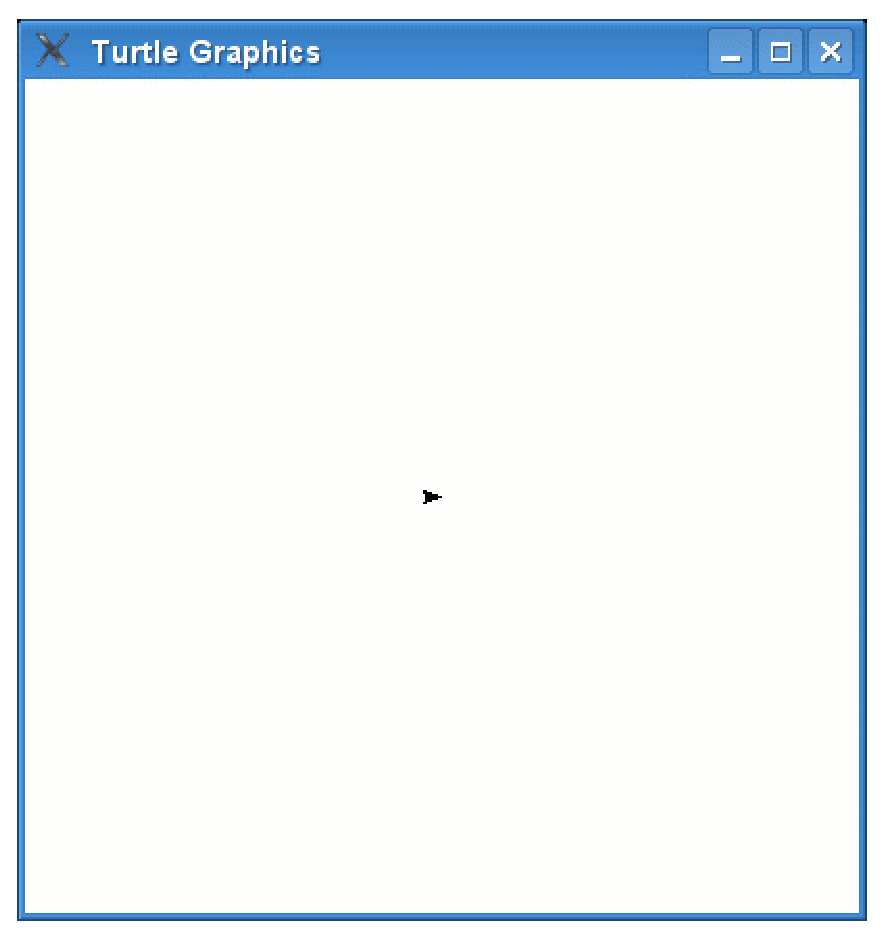
\includegraphics[width=72mm]{../en/figure10.eps}
\end{center}
\caption{Стрелочка, изображающая черепаху}\label{fig10}
\end{figure}

\btw{Да, эта маленькая стрелочке посреди экрана — действительно черепаха. И да, на черепаху она внешне не похожа примерно ничем.}

Этой черепахе можно отправлять инструкции, используя функции созданного объекта \code{t}. Вот, например, можно попросить черепаху продвинуться вперёд, туда, куда показывает стрелочка. Для этого есть функция \code{forward}, в скобках которой надо указать, на сколько точек на экране продвинуться. Например, чтобы подвинуть черепаху вперёд на 50 точек (и нарисовать линию длиной 50 точек), нужно выполнить такую команду:

\begin{listing}
\begin{verbatim}
>>> t.forward(50)
\end{verbatim}
\end{listing}

И в результате должно получиться как-то так:~\ref{fig11}.

\begin{figure}
\begin{center}
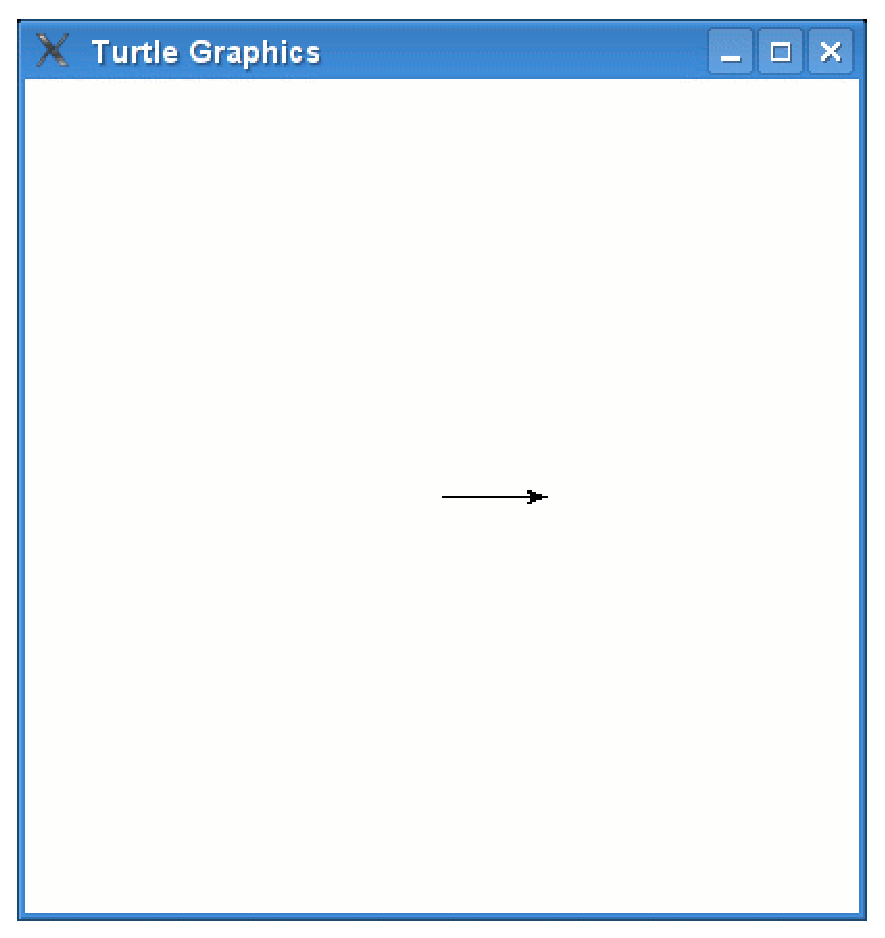
\includegraphics[width=72mm]{../en/figure11.eps}
\end{center}
\caption{Черепашка нарисовала линию.}\label{fig11}
\end{figure}

С точки зрения черепахи, она прошла вперёд 50 шагов. А мы бы сказали, что она прошла 50 точек по экрану.

\btw{И что это за точки такие?}

Всё на экране компьютера состоит из отдельных маленьких точек, каждая из которых окрашена в свой цвет. Обычно их называют пикселями, чтобы не путать ни с какими другими точками, и так я и буду дальше делать. Все программы на компьютере, все игры заставляют точки на экране окрашиваться в разные нужные цвета. Эти отдельные точки можно увидеть, вооружившись лупой. Если сильно увеличить линию, нарисованную черепахой, то можно увидеть, что это много квадратных точек, оказавшихся рядом, как на картинке \ref{fig12}.

\begin{figure}
\begin{center}
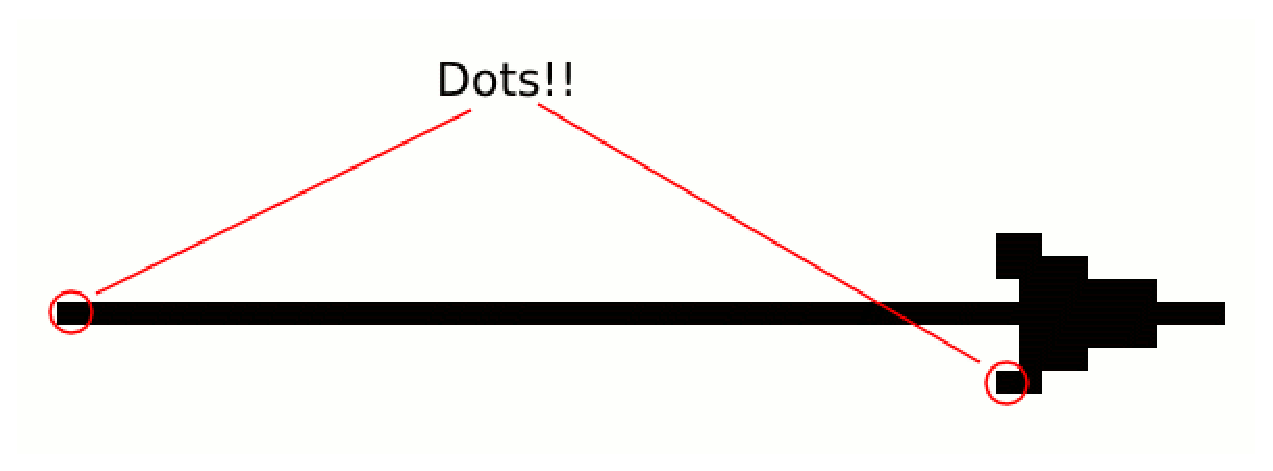
\includegraphics[width=72mm]{../en/figure12.eps}
\end{center}
\caption{Сильно увеличенные линия и стрелочка.}\label{fig12}
\end{figure}

В следующих главах мы ещё вспомним про пиксели, они нам пригодятся.

Вернёмся к черепашке. Её ещё можно попросить повернуть направо\index{черепашка!поворот направо} и налево\index{черепашка!поворот налево}.

\begin{listing}
\begin{verbatim}
>>> t.left(90)
\end{verbatim}
\end{listing}

Эта команда говорит черепашке повернуть налево на 90 градусов (то есть против часовой стрелки). Если ты ещё не знаешь про градусы\index{градусы} и как ими меряют углы, то это можно представить себе вот как. На рисунке \ref{fig13} есть циферблат от часов.

\begin{figure}
\begin{center}
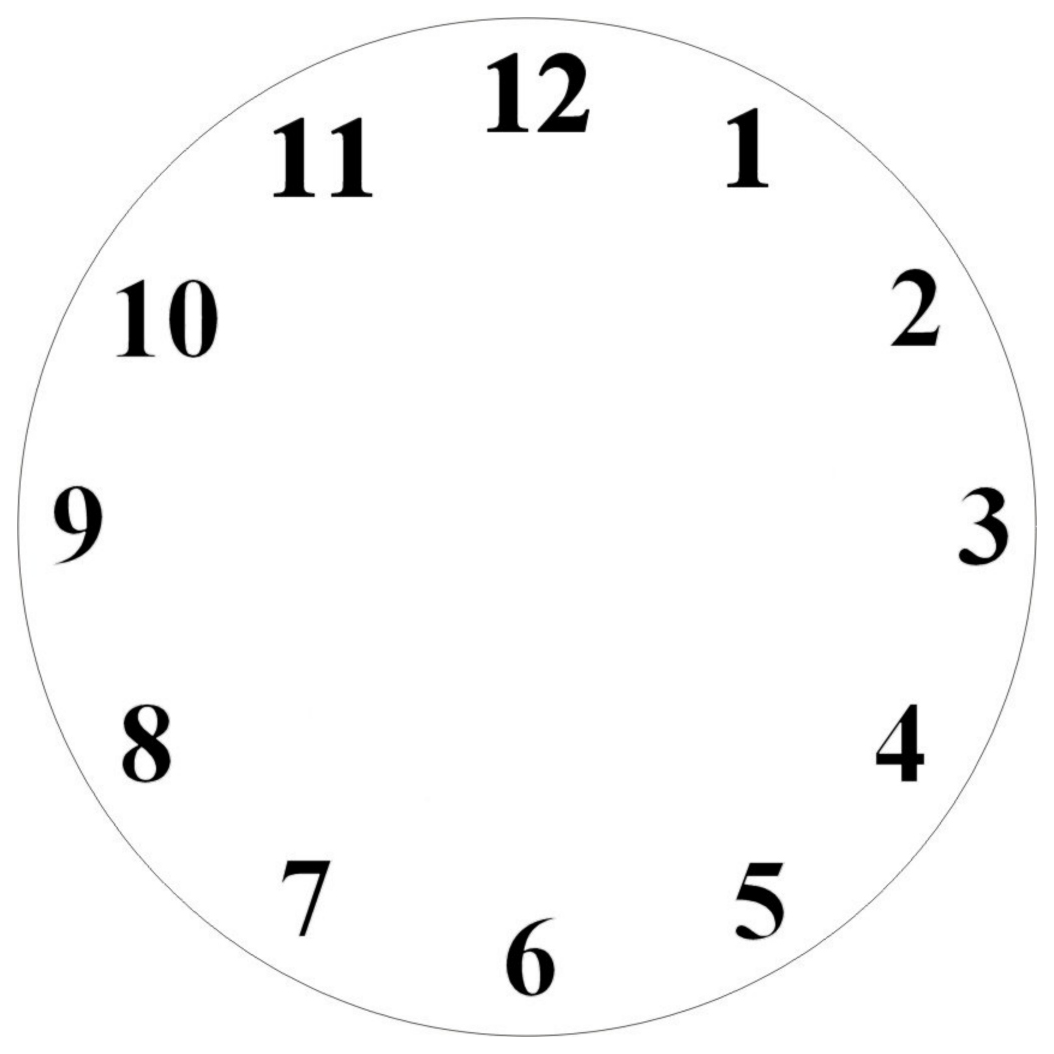
\includegraphics[width=52mm]{../en/figure13.eps}
\end{center}
\caption{Циферблат с отметками часов}\label{fig13}
\end{figure}

На циферблате по кругу написаны числа от 1 до 12 (или до 60, если там написаны минуты). Так вот градусы пишутся так же по кругу, только всё умножается на 30. Вместо цифры 3 — 90° (90 градусов), вместо шести — 180°, как на рисунке \ref{fig14}. А черепашка как будто стоит в центре циферблата и смотрит в сторону нуля, наверх.

\begin{figure}
\begin{center}
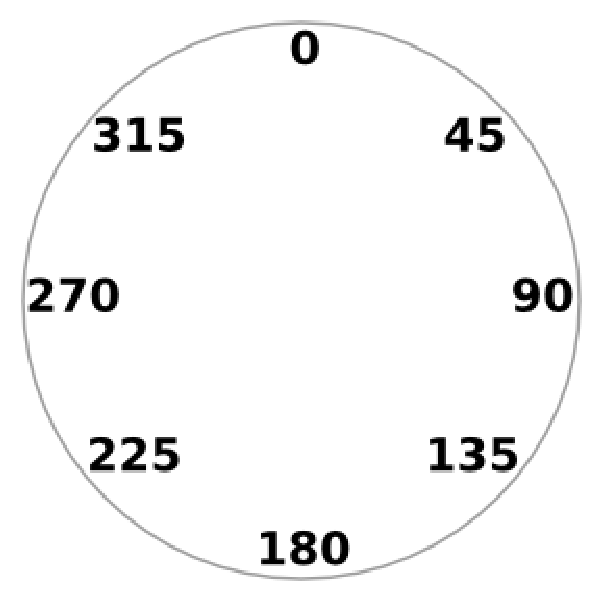
\includegraphics[width=52mm]{../en/figure14.eps}
\end{center}
\caption{Градусы.}\label{fig14}
\end{figure}

И что происходит, когда мы отдаём команду \code{left(90)}?

Если встать, поднять руку ровно в сторону и показать туда, то чтобы повернуться лицом в ту сторону, в которую ты показываешь, нужно повернуться как раз на 90 градусов. Если показывать правой рукой, то на 90° вправо, левой рукой — на 90° влево. Так же и черепашка в питоне поворачивается туда, где её правый бок или левый. При этом голова черепашки остаётся на месте (рисует она как раз маркером, зажатым в зубах), так что функция \code{t.left(90)} приводит к тому, что есть на рисунке \ref{fig15}. Черепашка ползла вправо и повернула вверх.

\begin{figure}
\begin{center}
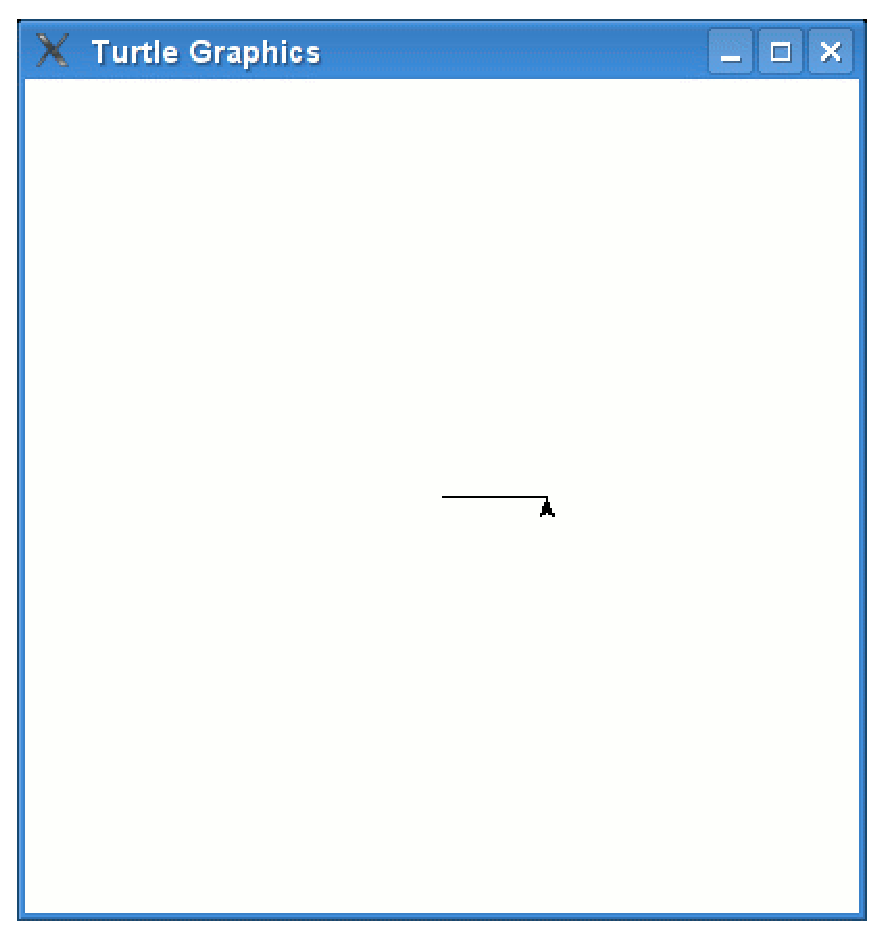
\includegraphics[width=72mm]{../en/figure15.eps}
\end{center}
\caption{Черепашка, повернувшая налево.}\label{fig15}
\end{figure}

Давай теперь посмотрим, как все эти команды работают вместе:

\begin{listing}
\begin{verbatim}
>>> t.forward(50)
>>> t.left(90)
>>> t.forward(50)
>>> t.left(90)
>>> t.forward(50)
>>> t.left(90)
\end{verbatim}
\end{listing}

На экране черепашка нарисовала квадрат и остановилась, глядя в ту же сторону, что и в начале пути, как на рисунке \ref{fig16}.

\begin{figure}
\begin{center}
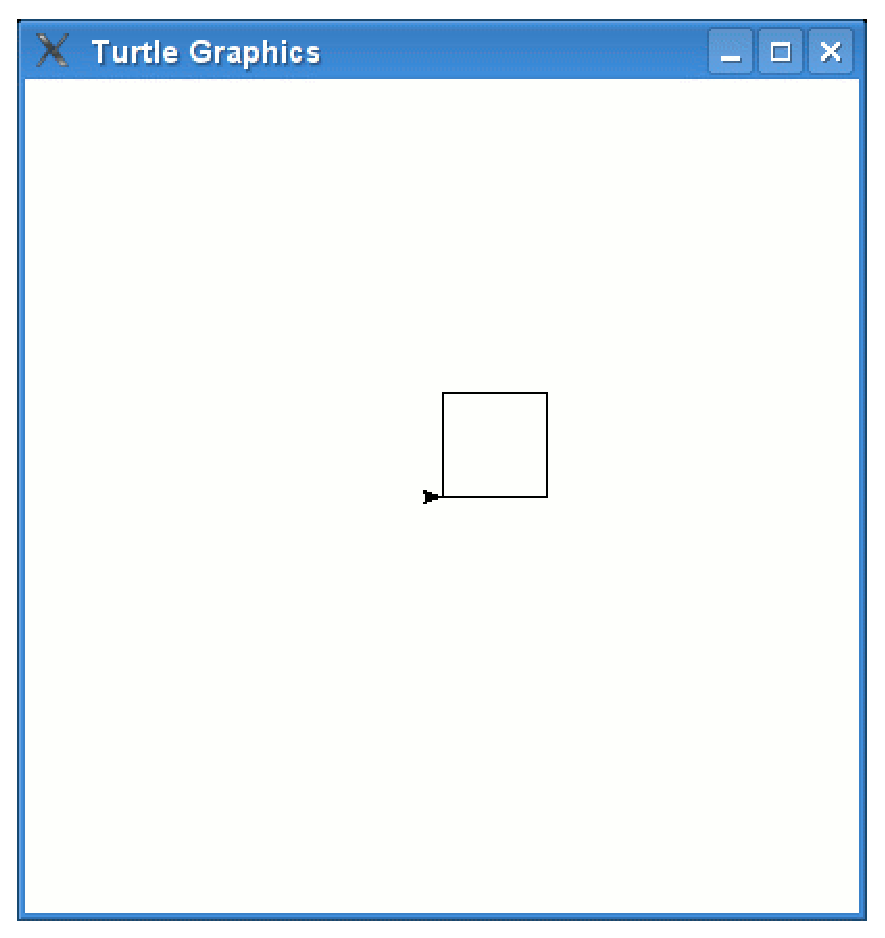
\includegraphics[width=72mm]{../en/figure16.eps}
\end{center}
\caption{Квадрат нарисовался.}\label{fig16}
\end{figure}

Можно взять и очистить весь холст, воспользовавшись функцией \code{clear}\index{черепашка!очистить} (что как раз и переводится как «очистить»):

\begin{listing}
\begin{verbatim}
>>> t.clear()
\end{verbatim}
\end{listing}

Есть и другие полезные функции, применимые к черепашке. Например, \code{reset}\index{черепашка!reset}: тоже очищает экран и ещё перемещает черепашку в начальное положение. Ещё есть функция \code{backward}, которая говорит черепашке двигаться назад (при этом направление её взгляда не меняется, она просто пятится). Функция \code{right} говорит черепашке повернуть направо; функция \code{up}\index{черепашка!прекратить рисовать} говорит ей оторвать маркер от холста, то есть перестать рисовать при движении: не всё можно нарисовать, если рисовать при каждом движении, иногда нужно просто переместиться. Есть и функция \code{down}\index{черепашка!начать рисовать}, которая говорит ей обратно опустить маркер на холст и снова рисовать, пока она перемещается. Все эти функции вызываются таким же образом, как в примерах выше:

\begin{listing}
\begin{verbatim}
>>> t.reset()
>>> t.backward(100)
>>> t.right(90)
>>> t.up()
>>> t.down()
\end{verbatim}
\end{listing}

В следующих главах мы ещё воспользуемся услугами черепашки.

\section{Чем развлечься на досуге}

\btw{В этой главе мы познакомились с маленькой черепашкой, которая нарисовала нам немного линий, поворачиваясь направо и налево. Ещё мы обсудили градусы, которые здорово похожи на числа на циферблате часов.}

\subsection*{Упражнение 1}
Создай холст, используя функцию \code{Pen}, и нарисуй там прямоугольник.

\subsection*{Упражнение 2}
Создай холст, используя функцию \code{Pen}, и нарисуй там треугольник.

\subsection*{Упражнение 3*}
Создай холст, используя функцию \code{Pen}, и нарисуй там домик, как на рисунке \ref{fighouse}, не отрывая маркер от холста (не пользуясь функцией \code{up}). Это упражнение сложнее предыдущих и может не получиться без посторонней помощи, ничего страшного\footnote{Чтобы всё получилось, нужно иметь в виду, что может понадобиться повернуть на 45 или 135 градусов и что если стороны домика длиной 100 точек, то косые линии будут длиной примерно 71 и 141 точка.}.

\begin{figure}
\begin{center}
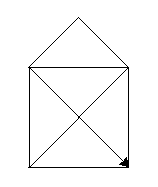
\includegraphics[width=72mm]{03.house.png}
\end{center}
\caption{Домик, который нарисовали, не отрывая карандаш от бумаги.}\label{fighouse}
\end{figure}

\newpage

% !TeX encoding = UTF-8
% Use XeLaTeX to compile it
%
% Эта работа распространяется на условиях лицензии Creative Commons Attribution-Noncommercial-Share Alike 3.0 New Zealand License.
% Краткое описание лицензии есть тут: http://creativecommons.org/licenses/by-nc-sa/3.0/nz/deed.ru
% Полное — там же.
% Эту книгу можно невозбранно распространять и изменять, но только соблюдая следующие условия:
% сохраняя лицензию и не вводя дополнительных ограничений, бесплатно
% и указывая авторство как оригинальной части, так и изменённой.
% Автор оригинального английского текста — Jason R Briggs http://jasonrbriggs.com/
% Автор перевода — Егор Кочетов <Egor.Kochetoff@gmail.com>
%
% This work is licensed under the Creative Commons Attribution-Noncommercial-Share Alike 3.0 New Zealand License.
% To view a copy of this license, visit http://creativecommons.org/licenses/by-nc-sa/3.0/nz
% or send a letter to Creative Commons, 171 Second Street, Suite 300, San Francisco, California, 94105, USA.
%

\chapter{Как задать вопрос}\label{ch:howtoaskaquestion}

С точки зрения программистов, вопрос задаётся тогда, когда в зависимости от ответа нужно выполнить одни команды или другие. Во многих языках программирования такой вопрос записывается с использованием слова \code{if}\index{if}, что на русский переводится как «если»\footnote{В некоторых языках прямо по-русски и пишут «если», но всё же обычно так не принято делать. В Питоне надо писать \code{if}.}. Такое выражение ещё называется \textbf{условным оператором}.

\begin{quotation}
Сколько тебе лет? Если тебе больше двадцати, ты супер стар!
\end{quotation}

Утверждение выше на Питоне может быть записано вот так:

\begin{listing}
\begin{verbatim}
if возраст > 20:
    print('ты супер стар!')
\end{verbatim}
\end{listing}

Условный оператор состоит из слова \code{if}, после которого записывается условие, завершаемое двоеточием (\code{:}). Все следующие строки, которые выполняются в зависимости от этого условия, должны начинаться с одинакового количества пробелов. Большинство людей использует тут 4 пробела, потому что так уже легко видеть \textit{блок кода}, и при этом он не слишком далеко уезжает направо. Для вставки такого отступа в начало строки обычно используют клавишу \texttt{Tab}, она на клавиатуре слева (←) под цифрами, слева от буквы Й.

Если ответ на вопрос, который написан после \code{if}, — да, или \code{True}, как это записывается в Питоне, то блок кода, начинающийся с отступов, выполняется.

Условие, которое надо писать после \code{if}, — это выражение, на которое можно ответить «да» (\code{True}, «истина») или «нет» (\code{False}, «ложь»). Чтобы записывать условия, есть специальные значки, вот они:

\begin{center}
\begin{tabular}{|c|c|}
\hline
$==$ & равно \\
\hline
$!=$ & не равно \\
\hline
$>$ & больше чем \\
\hline
$<$ & меньше чем \\
\hline
$>=$ & больше чем или равно \\
\hline
$<=$ & меньше чем или равно \\
\hline
\end{tabular}
\end{center}

Например, если тебе 10 лет, то условие \code{твой\_возраст == 10} истинно (равно \code{True}). Если же тебе не 10 лет, то оно ложно (равно \code{False}). Тут есть хитрость: чтобы сравнить два числа, надо написать два знака равенства подряд. Если написать только один, будет ошибка. А один знак нужно писать, чтобы в переменную занести какое-нибудь значение, то есть никак не после \code{if}.

Теперь допустим, что тебе больше 10 лет и в переменной \code{age} хранится твой возраст. Тогда вот такое условие…

\begin{listing}
\begin{verbatim}
age > 10
\end{verbatim}
\end{listing}

…будет равно \code{True}. А если тебе меньше 10 лет, то это условие будет равно \code{False}. И если тебе 10 лет, условие тоже будет ложно, зато будет истинно условие \code{age>=10}.

Давай попробуем теперь ввести примеры в консоль:

\begin{listing}
\begin{verbatim}
>>> age = 10
>>> if age > 10:
...     print('я тут!')
\end{verbatim}
\end{listing}

Если ввести это в консоль, что произойдёт?..

Да ничего.

Переменная \code{age} не больше 10, так что \code{print} не выполнится. А как насчёт такого:

\begin{listing}
\begin{verbatim}
>>> age = 10
>>> if age >= 10:
...     print('тут я!')
\end{verbatim}
\end{listing}

Вот если этот пример запустить, то Питон выведет сообщение в консоль. И следующий пример тоже сработает:

\begin{listing}
\begin{verbatim}
>>> age = 10
>>> if age == 10:
...     print('вот я где!')
вот я где!
\end{verbatim}
\end{listing}

\section{Сделай вот это… ИЛИ ВОТ ЭТО!}

Можно расширить условный оператор и сказать Питону, что делать, когда условие ложно. Можно, например, напечатать в консоль «Привет», если тебе 12 лет или «Пока» в ином случае. Для этого пригодится слово \code{else} (в переводе — «иначе»)\index{else}.

\begin{listing}
\begin{verbatim}
>>> age = 12
>>> if age == 12:
...     print('Привет!')
... else:
...     print('Пока.')
Привет!
\end{verbatim}
\end{listing}

Если ты напечатаешь в консоль этот пример, то увидишь в ответ «Привет!». Стоит изменить значение переменной \code{age} на что-нибудь другое, как сообщение от Питона поменяется:

\begin{listing}
\begin{verbatim}
>>> age = 8
>>> if age == 12:
...     print('Привет!')
... else:
...     print('Пока.')
Пока.
\end{verbatim}
\end{listing}

\section{Сделай вот это… или ещё вот это… ИЛИ ВОТ ЭТО!}

Можно ещё дальше расширить условный оператор, используя слово \code{elif} (сокращение от «else if»). Например, можно вот так печатать, сколько тебе лет (да, не слишком полезно, но позволяет ухватить суть этого условного оператора):

\begin{listing}
\begin{verbatim}
 1. >>> age = 12
 2. >>> if age == 10:
 3. ...     print('похоже, тебе 10 лет')
 4. ... elif age == 11:
 5. ...     print('я знаю, тебе 11 лет')
 6. ... elif age == 12:
 7. ...     print('ух ты, а тебе 12 лет')
 8. ... elif age == 13:
 9. ...     print('тебе целых 13 лет!')
10. ... else:
11. ...     print('Столько люди не живут.')
12. ...
13. ух ты, а тебе 12 лет
\end{verbatim}
\end{listing}

В примере кода выше строка 2 проверяет, равно ли значение возраста 10. Если нет, то сразу после этого выполняется строчка 4, которая проверяет, равно ли значение возраста 11. Если нет — то проверяется условие в строке 6. Оно оказывается истинным, поэтому выполняется строка 7 и больше никаких проверок не производится.

\section{Комбинируем условия}\index{условия!комбинации}
Можно проверять внутри одного условия сразу несколько выражений. Для этого используются английские слова «и»: \code{and} и «или»: \code{or}. Так например, пример выше можно было бы записать следующим образом, объединив проверки в одно большое условие:

\begin{listing}
\begin{verbatim}
1. >>> if age == 10 or age == 11 or age == 12 or age == 13:
2. ...     print('Я знаю, тебе %s лет' % age)
3. ... else:
4. ...     print('Столько люди не живут.')
\end{verbatim}
\end{listing}

Если любое из условий в строке 1 истинно, то все следующие и не проверяются и выполняется блок кода, следующий за \code{if}, то есть строка 2 в этом примере. Если же все условия ложны, то выполнится блок кода под \code{else}, то есть строчка 4. Этот пример можно ещё сократить, воспользовавшись операциями сравнения $<=$ и $>=$:

\begin{listing}
\begin{verbatim}
1. >>> if age >= 10 and age <= 13:
2. ...     print('Тебе %s лет' % age)
3. ... else:
4. ...     print('А сколько же?')
\end{verbatim}
\end{listing}

Тут если твой возраст не меньше 10 лет и не больше 13, то Питон напечатает, сколько тебе лет, а иначе — удивится.

\section{Пустота}\index{None}

Есть ещё специальное значение, которое можно присвоить любой переменной, и о котором мы раньше не говорили: \textbf{ничего}.

Точно так же, как переменной можно присвоить числа, строки и списки, переменной можно присвоить и «ничего». В Питоне это записывается словом \code{None} и значит, что в переменной ничего нет (в других языках используют слова типа \code{nil}, \code{null}, \code{nullptr}). При этом значение этой переменной можно напечатать, как и значение любой другой, и это не вызовет ошибки, как было бы, если бы переменная вообще не была объявлена.

\begin{listing}
\begin{verbatim}
>>> myval = None
>>> print(myval)
None
\end{verbatim}
\end{listing}

Присвоить переменной \code{None} может быть нужно, чтобы указать, что переменная чему-то будет равна потом, но сейчас её значение неизвестно\footnote{Если же хочется вообще удалить переменную, то надо не присвоить ей \code{None}, а написать вот так (для переменной \code{myval}): \code{del myval}.}.

Вот пример: допустим, мы хотим сходить в кино втроём, и для этого нам надо скинуться деньгами, кому сколько не жалко. Когда все решат, сколько им не жалко, и положат сумму, например, в конверт, можно на эти деньги выбрать фильм и купить билеты (а чтобы показать все фильмы из ближайших кинотеатров, на которые хватит этих денег, вполне можно написать программу на Питоне). Так вот, для этого мы заведём три переменных для каждого из зрителей и запишем в них \code{None}, что будет значить, что человек ещё вообще не сдавал деньги (если бы мы записали туда 0, это бы значило, что человек не хочет и не будет сдавать денег):

\begin{listing}
\begin{verbatim}
>>> зритель1 = None
>>> зритель2 = None
>>> зритель3 = None
\end{verbatim}
\end{listing}

Теперь можно проверить, все ли сдали деньги, пользуясь \code{if}'ом:

\begin{listing}
\begin{verbatim}
>>> if зритель1 is None or зритель2 is None or зритель3 is None:
...     print('Надо подождать ещё, не все сдали деньги')
... else:
...     print('Мы собрали %s руб.' % (зритель1 + зритель2 + зритель3))
\end{verbatim}
\end{listing}

\code{if} проверяет, записано ли в какую-то переменную значение \code{None} и, если это так, сообщает об этом. Если же в каждую переменную записано, кто сколько сдал денег, то Питон напечатает нам общую собранную сумму.

Вот что будет, если только два человека решились:

\begin{listing}
\begin{verbatim}
>>> зритель1 = 100
>>> зритель2 = None
>>> зритель3 = 300
>>> if зритель1 is None or зритель2 is None or зритель3 is None:
...     print('Надо подождать ещё, не все сдали деньги')
... else:
...     print('Мы собрали %s руб.' % (зритель1 + зритель2 + зритель3))
Надо подождать ещё, не все сдали деньги
\end{verbatim}
\end{listing}

А вот, если все трое:

\begin{listing}
\begin{verbatim}
>>> зритель1 = 100
>>> зритель2 = 500
>>> зритель3 = 300
>>> if зритель1 is None or зритель2 is None or зритель3 is None:
...     print('Надо подождать ещё, не все сдали деньги')
... else:
...     print('Мы собрали %s руб.' % (зритель1 + зритель2 + зритель3))
Мы собрали 900 руб.
\end{verbatim}
\end{listing}

\section{В чём разница…?}\label{whatsthedifference}\index{равенство}

Какая разница между \code{10} и \code{'10'}?

Так вообще, кажется, что, кроме пары кавычек, её и нет. Хотя вот в предыдущих главах ты узнал, что \code{10} — это число, а \code{'10'} — строка. И это различие гораздо существеннее, чем можно подумать.

Недавно мы проверяли, чему равен возраст, вот так:

\begin{listing}
\begin{verbatim}
>>> if age == 10:
...     print('помни: тебе 10 лет')
\end{verbatim}
\end{listing}

И если в переменную \code{age} записать значение 10, то всё, что надо, на экране напечатается:

\begin{listing}
\begin{verbatim}
>>> age = 10
>>> if age == 10:
...     print('помни: тебе 10 лет')
...
помни: тебе 10 лет
\end{verbatim}
\end{listing}

Но если в ту же переменную записать \code{'10'} (с кавычками), то ничего печататься не будет:

\begin{listing}
\begin{verbatim}
>>> age = '10'
>>> if age == 10:
...     print('помни: тебе 10 лет')
...
\end{verbatim}
\end{listing}

Как же так? Почему теперь ничего не работает? Ну потому что строка — это не число, хотя и выглядят они одинаково:

\begin{listing}
\begin{verbatim}
>>> age1 = 10
>>> age2 = '10'
>>> print(age1)
10
>>> print(age2)
10
\end{verbatim}
\end{listing}

Вот, видишь! Выглядят совсем одинаково, если напечатать. Но число никогда не будет равно строке.

Это вроде как странно, но смысл какой-то такой, что если сравнивать 10 книг и 10 кирпичей, они никогда не будут равны — они просто разные. То есть можно сравнить 10 штук книг и 10 штук кирпичей — количество (число) одинаковое, но сказать, что 10 кирпичей — это одно и то же («равно»), что и 10 книг, вряд ли получится. Вот так и тут.

Но это не страшно, Питон умеет прочитать строку и понять, какое число там записано, и наоборот, записать цифрами число в строку. Вот так можно превратить строку \code{'10'} в число \code{10}:

\begin{listing}
\begin{verbatim}
>>> age = '10'
>>> converted_age = int(age)
\end{verbatim}
\end{listing}

Теперь переменная \code{converted\_age} хранит число 10 (не строку). Функция \code{int}, которая используется для такого преобразования, названа как сокращение от английского слова «integer», что значит «целое число», число без дробной части, без запятой.

Чтобы обратно перевести число в строку, есть функция \code{str} (сокращение от «string», «строка»):

\begin{listing}
\begin{verbatim}
>>> age = 10
>>> converted_age = str(age)
\end{verbatim}
\end{listing}

Теперь в переменной \code{converted\_age} лежит строка \code{'10'}. Самое время вернуться к тому сравнению, которое у нас не работало:

\begin{listing}
\begin{verbatim}
>>> age = '10'
>>> if age == 10:
...     print('Тебе %s лет' % age)
...
\end{verbatim}
\end{listing}

Если мы преобразуем переменную перед проверкой, тогда мы получим другой результат:

\begin{listing}
\begin{verbatim}
>>> age = '10'
>>> converted_age = int(age)
>>> if converted_age == 10:
...     print('Тебе %s лет' % age)
...
Тебе 10 лет
\end{verbatim}
\end{listing}

Или даже прямо так, короче и без дополнительной переменной:

\begin{listing}
\begin{verbatim}
>>> age = '10'
>>> if int(age) == 10:
...     print('Тебе %s лет' % age)
...
Тебе 10 лет
\end{verbatim}
\end{listing}

% ch5.tex
% This work is licensed under the Creative Commons Attribution-Noncommercial-Share Alike 3.0 New Zealand License.
% To view a copy of this license, visit http://creativecommons.org/licenses/by-nc-sa/3.0/nz
% or send a letter to Creative Commons, 171 Second Street, Suite 300, San Francisco, California, 94105, USA.


\chapter{Снова и снова}\label{ch:againandagain}

Нет ничего хуже, чем делать одно и то же много раз подряд, одинаково и монотонно. Примерно поэтому родители могли когда-нибудь советовать тебе считать воображаемых овец, пока ты не уснёшь (а вовсе не потому, что эти шерстяные животные обладают магическими способностями усыплять). Всё дело в том, что повторять без конца одно и то же — скучно, и твоё сознание скоро сдастся и уступит место сну.

Программисты тоже не большие любители повторять одни и те же действия. От этого их тоже клонит в сон. Так что почти во всех языках программирования есть такая штука как \textit{цикл}\footnote{Некоторые языки обходятся без циклов, а некоторые — и без переменных. Но, как я и говорила, о других языках тут мы поговорить просто не успеем.}. В частности, \textit{цикл for}. И вот зачем. Допустим, тебе захочется 5 раз напечатать «Привет». Можно было бы сделать это так:
\begin{listing}
\begin{verbatim}
>>> print("Привет")
Привет
>>> print("Привет")
Привет
>>> print("Привет")
Привет
>>> print("Привет")
Привет
>>> print("Привет")
Привет
\end{verbatim}
\end{listing}

Но так писать очень утомительно.

Вместо того, чтобы повторять кучу раз одно и то же, можно использовать цикл \code{for} (не забудь про 4 пробела во второй строчке перед \code{print}):

\begin{verbatim}
>>> for x in range(0, 5):
...     print('Привет')
... 
Привет
Привет
Привет
Привет
Привет
\end{verbatim}

Функция \code{range}\index{функции!range} — быстрый способ создать список чисел от начального значения (включительно) до конечного (не включительно). Вот пример:

\begin{listing}
\begin{verbatim}
>>> print(list(range(10, 20)))
[10, 11, 12, 13, 14, 15, 16, 17, 18, 19]
\end{verbatim}
\end{listing}

И в нашем цикле \code{for} на самом деле строчка \code{for x in range(0, 5)} говорит Питону создать список чисел \code{[0, 1, 2, 3, 4]}, сохранить по очереди каждое из этих чисел в переменной \code{x} и выполнить для каждого значения этой переменной блок кода, написанный под \code{for}. Переменную \code{x} тоже можно использовать для печати:

\begin{listing}
\begin{verbatim}
>>> for x in range(0, 5):
...     print('[%s] Привет' % x)
...
[0] Привет
[1] Привет
[2] Привет
[3] Привет
[4] Привет
\end{verbatim}
\end{listing}

Если явно записать то, что происходит в цикле \code{for}, то получится что-то такое:

\begin{listing}
\begin{verbatim}
x = 0
print('[%s] Привет' % x)
x = 1
print('[%s] Привет' % x)
x = 2
print('[%s] Привет' % x)
x = 3
print('[%s] Привет' % x)
x = 4
print('[%s] Привет' % x)
\end{verbatim}
\end{listing}

Так что цикл нас тут избавил от лишних восьми строк кода. И это невероятно полезно, потому что средний программист чуть более ленив, чем бегемот жарким днём, когда дело доходит до печатания кода. Хорошие программисты ненавидят делать одно и то же больше одного раза (и на то есть серьёзные причины\footnote{Например, если найдётся ошибка в каком-то коде, то исправить её нужно будет только один раз. Если один и тот же ошибочный код использовать несколько раз, то где-то ошибку точно забудут исправить.}), так что цикл — одна из самых полезных инструкций в языке программирования.

\fbox{\colorbox{PaleBlue}{\parbox{.75\linewidth} {
\subsection*{Аккуратней с пробелами!}

Возможно, ты пытался запустить примеры из этой главы и в качестве результата получил только сообщение об ошибке вроде такого:

\begin{listing}
IndentationError: expected an indented block
\end{listing}

Такая ошибка значит, что в начале строки не хватает пробелов, хотя бы одного. Пробелы в начале строки в Питоне очень важны. Скоро мы о них поговорим подробнее…
}}}
\linebreak

Можно не ограничиваться функцией \code{range} для цикла \code{for}, можно использовать и другие списки (которые мы раньше создавали). Вот, например, список покупок:

\begin{listing}
\begin{verbatim}
>>> shopping_list = [ 'яиц', 'молока', 'сыра', 'сельдерея', 'масла', 'соды' ]
>>> for i in shopping_list:
...     print("Как бы не забыть купить %s" % i)
Как бы не забыть купить яиц
Как бы не забыть купить молока
Как бы не забыть купить сыра
Как бы не забыть купить сельдерея
Как бы не забыть купить масла
Как бы не забыть купить соды
\end{verbatim}
\end{listing}

Этот код значит «сохрани по очереди каждый из элементов списка в переменной \code{i} и выполни \code{print} для каждого из значений».

Опять же, если бы мы решили делать это без списка, то пришлось бы печатать что-нибудь такое:

\begin{listing}
\begin{verbatim}
>>> shopping_list = [ 'яиц', 'молока', 'сыра', 'сельдерея', 'масла', 'соды' ]
>>> print("Как бы не забыть купить %s" % shopping_list[0])
Как бы не забыть купить яиц
>>> print("Как бы не забыть купить %s" % shopping_list[1])
Как бы не забыть купить молока
>>> print("Как бы не забыть купить %s" % shopping_list[2])
Как бы не забыть купить сыра
>>> print("Как бы не забыть купить %s" % shopping_list[3])
Как бы не забыть купить сельдерея
>>> print("Как бы не забыть купить %s" % shopping_list[4])
Как бы не забыть купить масла
>>> print("Как бы не забыть купить %s" % shopping_list[5])
Как бы не забыть купить соды
\end{verbatim}
\end{listing}

Так что \code{for} снова спас нас от кууучи лишнего кода.

\section{Зачем нужны блоки программистам?}\index{блоки кода}

Чтобы делать их из кода.

Что же такое «блок кода»?

Блок кода — это несколько программных инструкций, объединённых вместе. Например, в примере с циклом \code{for} может захотеться не только печатать, что надо купить, но и как-нибудь покупать. Предположим, что есть функция \code{buy} для этого (на самом деле её пока нет). Тогда можно записать этот пример вот так:

\begin{verbatim}
>>> for i in shopping_list:
...     buy(i)
...     print(i)
\end{verbatim}

Печатать это в консоль не стоит и пытаться, потому что функции \code{buy} нету, и результатом будет только сообщение об ошибке. Зато тут есть настоящий блок кода, вот этот:

\begin{verbatim}
    buy(i)
    print(i)
\end{verbatim}

В Питоне пробельные символы\index{пробельные символы}, а именно символ табуляции (который получается, если нажать клавишу Tab\footnote{В консоли Питона этот способ не сработает, только в текстовом редакторе так получится.}) и символ пробела, очень важны. Код с одинаковым отступом от начала строки автоматически группируется в блоки.

\begin{listing}
\begin{verbatim}
	это блок 1
	это блок 1
	это блок 1
	    это блок 2
	    это блок 2
	    это блок 2
	это всё ещё блок 1
	это всё ещё блок 1
	    это блок 3
	    это блок 3
	        это блок 4
	        это блок 4
	        это блок 4
\end{verbatim}
\end{listing}

Единственное правило тут — что нужно использовать одно и то же количество пробелов в начале строк внутри всего блока. Вот так неправильно:

\begin{verbatim}
>>> for i in shopping_list:
...     buy(i)
...       print(i)
\end{verbatim}

Отступ второй строки здесь 4 пробела, а третьей строки — 6 пробелов, её начало сдвинуто ещё на 2 символа вправо. Такой код вызовет ошибку. Если уж блок начался с отступом в 4 пробела, то так он и должен продолжаться. А если хочется внутри блока поместить другой, то нужно будет использовать 8 пробелов (два раза по четыре) в начале строк этого внутреннего блока. Вот так правильно:

\begin{listing}
\begin{verbatim}
    вот первый блок кода
    вот первый блок кода
\end{verbatim}
\end{listing}

И вот блок кода, в который вложен ещё один. Все строчки в нём начинаются с 8 пробелов:

\begin{listing}
\begin{verbatim}
    вот первый блок кода
    вот первый блок кода
        вот второй блок кода
        вот второй блок кода
\end{verbatim}
\end{listing}

Зачем может захотеться вложить один блок кода в другой? Обычно это случается, когда второй блок зависит от первого. Например, если второй блок — тело цикла \code{for}. Строчка со словом \code{for} находится в первом блоке кода, а всё, что должно выполняться в цикле, нужно поместить во второй блок.

Если ты начинаешь блок в консоли Питона, то Питон продолжает этот блок до тех пор, пока ты не нажмёшь
Enter в пустой строке. Каждую строчку блока при этом Питон начинает с трёх точек.

Давай попробуем ввести в консоль пример. Напечатай туда код, написанный ниже, не забывая про 4 пробела в начале строк в блоке кода после \code{for}\footnote{Вообще, в консоли хватит и одного пробела. Для блока, вложенного в первый, — двух пробелов и так далее. 4 пробела используют в программах, которые сохраняют в файлы и которые потом люди будут читать ещё раз.}.

\begin{listing}
\begin{verbatim}
>>> mylist = [ 'a', 'b', 'c' ]
>>> for i in mylist:
...     print(i)
...     print(i * 3)
...
a
aaa
b
bbb
c
ccc
\end{verbatim}
\end{listing}

После второй строчки с \code{print} нужно нажать Enter на пустой строке — так Питон поймёт, что ты хочешь завершить блок. И напечатает всё, что просили.

Следующий пример вызовет ошибку:

\begin{listing}
\begin{verbatim}
>>> mylist = [ 'a', 'b', 'c' ]
>>> for i in mylist:
...     print(i)
...       print(i)
...
File “<stdin>”, line 3
  print(i)
  ^
IndentationError: unexpected indent
\end{verbatim}
\end{listing}

В начале второй строчки с командой \code{print} вместо четырёх пробелов шесть, что Питону крайне не нравится: отступы должны быть одинаковыми, какие бы они ни были.

\fbox{\colorbox{PaleBlue}{\parbox{.75\linewidth} {
\subsection*{Запомни}

Если ты используешь четыре пробела, чтобы сделать отступ для одного из блоков кода, то все следующие блоки нужно тоже начинать с четырёх пробелов. Если же для отступов используются два пробела, то два и нужно использовать во всей программе. Большинство людей используют четыре пробела, чего я и тебе советую.
}}}

Вот пример чуть посложнее с двумя блоками кода:

\begin{listing}
\begin{verbatim}
>>> mylist = [ 'a', 'b', 'c' ]
>>> for i in mylist:
...     print(i)
...     for j in mylist:
...         print(j)
...
\end{verbatim}
\end{listing}

Где в этом коде блоки и что он делает?..

Блоков два. Первый — часть первого цикла \code{for}:

\begin{listing}
\begin{verbatim}
>>> mylist = [ 'a', 'b', 'c' ]
>>> for i in mylist:
...     print(i)                #
...     for j in mylist:        #<-- все эти строки — это первый блок кода
...         print(j)            #<-- эта строка — тоже часть первого блока
...
\end{verbatim}
\end{listing}

Второй блок состоит из одной строки, выполняющейся во вложенном цикле \code{for}:

\begin{listing}
\begin{verbatim}
>>> mylist = [ 'a', 'b', 'c' ]
>>> for i in mylist:
...     print(i)
...     for j in mylist:
...         print(j)               #<-- вот эта строка — второй блок кода
...
\end{verbatim}
\end{listing}

Можешь ли ты понять, глядя на этот код, что он делает?

Он напечатает каждую из трёх букв из списка, но сколько раз? Если мы внимательно посмотрим на код, то, скорее всего, сможем ответить на этот вопрос. Мы знаем, что первый цикл \code{for} выполнится для каждой буквы один раз. Он напечатает эту букву, а потом запустит вложенный цикл. А вложенный цикл опять выполнится по разу для каждой буквы и просто её напечатает. Получается, что сначала на экране появится буква 'a', затем — по очереди буквы 'a', 'b', 'c'. Потом — буква 'b' и опять все три и потом — буква 'c'. Можешь ввести этот код в консоль Питона и собственноручно убедиться, что всё так и будет.

\begin{listing}
\begin{verbatim}
>>> mylist = [ 'a', 'b', 'c' ]
>>> for i in mylist:
...     print(i)
...     for j in mylist:
...         print(j)
... 
a
a
b
c
b
a
b
c
c
a
b
c
\end{verbatim}
\end{listing}

Кажется, я слышу вопрос, можно ли использовать циклы для чего-то немного более полезного, чем печать букв одной за одной? Можно, конечно, иначе бы и не стали циклы придумывать. Вспомни пример из второй главы, когда мы считали, сколько карманных денег накопится к концу года. Там тебе платили 5 рублей в неделю за домашние дела, 30 рублей в неделю за разнос газет, и ещё ты тратил 10 рублей в неделю.

К концу года копилась вот такая сумма:

\begin{listing}
\begin{verbatim}
>>> (5 + 30 - 10) * 52
\end{verbatim}
\end{listing}

\noindent
(5 рублей + 30 рублей − 10 рублей, и всё это умножить на 52 недели в году).

Может захотеться посмотреть, сколько денег накопится в каждую из недель года, чтобы прикинуть, насколько быстро удастся накопить на ту или иную вещь, и выбрать: на что копить, чтобы было не слишком долго (и сколько именно придётся копить). Этого можно добиться, как раз используя цикл for. Однако прежде всего надо сохранить все эти числа в переменные\footnote{В любых программах не принято использовать числа или строки просто так. Их сохраняют в переменные. Во-первых, так сразу видно, что значит число (если переменная названа понятно); во-вторых, его легко поменять всего в одном месте.}:

\begin{listing}
\begin{verbatim}
>>> chores = 5
>>> paper = 30
>>> spending = 10
\end{verbatim}
\end{listing}

Теперь исходный пример записывается так:

\begin{listing}
\begin{verbatim}
>>> (chores + paper - spending) * 52
1300
\end{verbatim}
\end{listing}

А увидеть, сколько денег накопится в каждую из недель, можно так:

\begin{listing}
\begin{verbatim}
1. >>> savings = 0
2. >>> for week in range(1, 53):
3. ...     savings = savings + chores + paper - spending
4. ...     print('В конце недели № %s будет %s рублей' % (week, savings))
5. ...
\end{verbatim}
\end{listing}

В строке 1 в переменную savings заносится начальное значение: 0 (ещё ничего не накопилось).

В строке 2 записан цикл \code{for}, который выполнится по разу для каждой из недель в году. На каждом шаге цикла переменная \code{week} будет иметь значение от 1 до 52\footnote{range(1,53) возвращает список чисел от 1 включительно до 53 не включительно, то есть [0,...,52].}.

В строке 3 к тому, что мы уже накопили, прибавляется ещё то, что накопится в очередную неделю. Иными словами, в переменную \code{savings} записывается столько, сколько там уже было, и ещё столько, сколько добавится на этой неделе. Знак равенства «\code{=}» говорит Питону посчитать всё, что справа от этого знака, и сохранить результат в переменную слева — и именно в таком порядке. Так что если и справа и слева от знака равенства есть одна и та же переменная, ничего страшного.

% TODO
% Вот оригинальный фрагмент текста, я не нашёл в себе силы перевести его более точно — welcome (clone, push, merge)
%Line 3 is a bit more complicated.  Basically, each week we want to add what we've saved to our total savings.  Think of the variable `savings' as something like a bank.  We add up the money we earn doing odd jobs and the paper route, subtract our spending money and then take the rest to the bank.  So in computer-speak, line 3 really means, ``replace the contents of the variable savings with my current savings, plus what I've earned this week''. Basically, the equals symbol (=) is a bossy piece of code that is a way of saying, ``work out some stuff on the right first and then save it for later, using the name on the left''.\\
В строке 4 печатается результат расчётов: сколько денег будет в конце каждой недели, считая с нынешней.
%TODO перевести ссылку:
%Check the section \emph{Tricks with Strings} on page~\pageref{trickswithstrings}, if this line doesn't make a lot of sense to you.

Если теперь запустить эту программу, получится вот что:

\begin{listing}
\begin{verbatim}
В конце недели № 1 будет 25 рублей
В конце недели № 2 будет 50 рублей
В конце недели № 3 будет 75 рублей
В конце недели № 4 будет 100 рублей
В конце недели № 5 будет 125 рублей
В конце недели № 6 будет 150 рублей
В конце недели № 7 будет 175 рублей
В конце недели № 8 будет 200 рублей
В конце недели № 9 будет 225 рублей
В конце недели № 10 будет 250 рублей
В конце недели № 11 будет 275 рублей
В конце недели № 12 будет 300 рублей
В конце недели № 13 будет 325 рублей
В конце недели № 14 будет 350 рублей
В конце недели № 15 будет 375 рублей
\end{verbatim}
\end{listing}

…и так далее до 52-й недели.


\section{Пока мы тут говорим про циклы…}\index{while-loop}

Циклом \code{for} в питоне дело не ограничивается. Есть ещё цикл \code{while} (что по-русски значит «пока» или «в то время как»). В Питоне для цикла \code{for} заранее известно, когда он остановится: когда переберёт все элементы (или раньше, если его прервать, но никак не позже). Цикл \code{while} используется в тех случаях, когда заранее непонятно, когда остановиться.

Представь себе освещённую лестницу из 20 ступенек. И представь, что по ней нужно подняться, печатая номер каждой очередной ступеньки\footnote{Между прочем, это уже вполне реальная ситуация. Когда роботов учат подниматься по лестнице, что даётся им непросто, после подъёма на каждую очередную ступеньку робот проверяет, что он не упал, и печатает номер ступеньки. Или понимает, что упал, и печатает номер ступеньки, на которой упал. Потом его программу улучшают так, чтобы он не падал.}. Если мы представим, что есть команда \code{step\_up()}, которую нужно вызвать, чтобы сделать шаг, то всё это можно записать таким циклом \code{for}:

\begin{listing}
\begin{verbatim}
>>> for step in range(0,20):
...     step_up()
...     print(step)
\end{verbatim}
\end{listing}

А теперь представь, что эта лестница не освещена; неизвестно, сколько в ней ступенек, а идти нужно до первой двери, а потом уйти в эту дверь с лестницы (и вообще, это длинная-длинная винтовая лестница в старинной магической башне). Тут не получится использовать цикл \code{for}, потому что наперёд неизвестно, сколько всего ступенек. Тут-то и нужен \code{while}:

\begin{verbatim}
>>> step = 0
>>> while no_door():
...     step_up()
...     print(step)
...     if tired():
...         break
...     else:
...         step = step + 1
>>> print('Остановились на ступеньке %s' % step)
\end{verbatim}

Этот код нет смысла запускать, потому что он использует выдуманные функции: \code{no\_door()}~— эта функция проверяет, есть ли дверь, и возвращает \code{True}, если её нет — и \code{tired()} — эта функция возвращает \code{True}, если сил идти вверх больше нет. Но этот код показывает смысл цикла \code{while}. Пока условие истинно, то есть пока \code{no\_door()} — правда, цикл выполняется. Внутри цикла мы проверяем, есть ли ещё силы идти вверх, и если нет, то тут же и прерываем цикл (\code{break}) и переходим к самой последней строчке кода. Потом, за циклом мы можем ещё раз проверить \code{no\_door}, чтобы понять, почему цикл завершился: надо ли войти в дверь или отдохнуть и идти дальше. Если же силы идти есть, то номер ступеньки увеличивается, и мы делаем следующий шаг.

Итак, цикл \code{while} устроен следующим образом:

{\renewcommand{\labelitemi}{$\triangleright$}
\begin{itemize}
\item проверить условие,
\item выполнить блок кода,
\item повторить всё с начала.
\end{itemize}}

Часто цикл \code{while} проверяет сразу несколько условий. Например, так:

\begin{listing}
\begin{verbatim}
>>> x = 45
>>> y = 80
>>> while x < 50 and y < 100:
...     x = x + 1
...     y = y + 1
...     print(x, y)
\end{verbatim}
\end{listing}

Тут есть две переменные и два условия, по одному для каждой. В цикле переменная \code{x} изменяется от 45 до 50, а \code{y} — от 80 до 100. Когда первая из переменных достигнет своего максимального значения (50 для \code{x} и 100 для \code{y}), цикл тут же завершится.

\begin{listing}
\begin{verbatim}
46 81
47 82
48 83
49 84
50 85
\end{verbatim}
\end{listing}

Наверное, не стоит тебе надоедать излишне подробными объяснениями, почему напечатались именно эти строки\footnote{…или всё-таки стоит? Вначале \code{x} равняется 45, а \code{y} — 80. Обе переменные увеличиваются на 1 на каждом шаге цикла и печатаются. Так и получается то, что напечатано. Когда \code{x} равно 50, условие \code{x < 50} перестаёт быть истинным (\code{True}), поэтому и всё вместе условие цикла «\code{x < 50 и y < 80}» тоже перестаёт быть истинным, и цикл завершается.}.

Ещё \code{while} используют, чтобы создать бесконечный цикл или почти бесконечный, вот так:

\begin{verbatim}
>>> while True:
...     lots of code here
...     lots of code here
...     lots of code here
...     if some_condition == True:
...         break
\end{verbatim}

Условие для этого цикла \code{while} — просто «\code{True}». Это условие всегда выполняется, и тело цикла всегда будет запускаться, это вечный цикл. Но как только переменная \code{some\_condition} тоже примет значение \code{True}, цикл прервётся инструкцией \code{break}.

%TODO перевести предложение ниже (и ссылку)
%You can see a better example of this in Appendix~\ref{app:afewpythonmodules} (the section about the \code{random} module), but you might want to wait until you've read the next chapter before taking a look at it.

\section{Что ещё попробовать}

\btw{В этой главе мы увидели, как использовать циклы, чтобы выполнять повторяющиеся действия. Мы использовали блоки кода внутри циклов для записи этих действий.}

\subsection*{Упражнение 1}
Как ты думаешь, что произойдёт, если запустить этот код:

\begin{listing}
\begin{verbatim}
>>> for x in range(0, 20):
...     print('hello %s' % x)
...     if x < 9:
...         break
\end{verbatim}
\end{listing}

\subsection*{Упражнение 2}
Если положить деньги в банк, то банк за них платит проценты — за то, что он может ими пользоваться на своё усмотрение и давать кому-то в долг (под большие проценты). Каждый месяц банк добавляет на твой счёт какую-то небольшую часть от того, что на нём уже лежит. Например, если положить в банк 1000 рублей, то банк добавляет каждый месяц ещё по 10 рублей (сколько именно, зависит от банка, но примерно столько или меньше).

Так вот, когда ты кладёшь деньги в банк, он сообщает тебе, сколько \emph{процентов} в год банк добавит. Допустим, ты положил 1000 рублей, и банк добавит 5\% в год — тогда через год у тебя будет $1000 + 1000×0.05$ рублей. Если банк обещает добавить 10\%, то через год у тебя будет $1000+1000×0.10$ рублей — и так далее. Предположим, проценты выплачиваются в конце каждого года (хотя это и не так, но так проще считать и результаты получаются почти точные). Тогда, если ты положишь 1000 рублей под 7\% годовых, через год у тебя будет $1000+1000×0.07$. Потом ещё через год банк добавит 7\% уже на эту сумму. Ещё через год — на сумму, оставшуюся в конце второго года, — и так далее. В уме это посчитать сложно; а в жизни такая задача возникает часто.

Напиши программу, которая посчитает, сколько на счёте накопится денег через 10 лет, если положить 10 000 рублей под 7\% годовых (не забудь, что каждый год проценты считаются от той суммы, что лежала в конце прошлого года, а не в самом начале всех этих 10 лет).
\newpage
% !TeX encoding = UTF-8
% Use XeLaTeX to compile it
%
% Эта работа распространяется на условиях лицензии Creative Commons Attribution-Noncommercial-Share Alike 3.0 New Zealand License.
% Краткое описание лицензии есть тут: http://creativecommons.org/licenses/by-nc-sa/3.0/nz/deed.ru
% Полное — там же.
% Эту книгу можно невозбранно распространять и изменять, но только соблюдая следующие условия:
% сохраняя лицензию и не вводя дополнительных ограничений, бесплатно
% и указывая авторство как оригинальной части, так и изменённой.
% Автор оригинального английского текста — Jason R Briggs http://jasonrbriggs.com/
% Автор перевода — Егор Кочетов <Egor.Kochetoff@gmail.com>
%
% This work is licensed under the Creative Commons Attribution-Noncommercial-Share Alike 3.0 New Zealand License.
% To view a copy of this license, visit http://creativecommons.org/licenses/by-nc-sa/3.0/nz
% or send a letter to Creative Commons, 171 Second Street, Suite 300, San Francisco, California, 94105, USA.
%

\chapter{Повторное использование…}\label{ch:sortoflikerecycling}

Представь, сколько мусора ты производишь каждый день. Всякие бутылочки от воды, обёртки от еды, пакетики от овощей, пластиковые коробочки, в которых продают мясо; а ещё, возможно, журналы, газеты или другая бумага. Ну и теперь представь, что получится, если этот весь мусор сложить в одну большую кучу.

\begin{center}
\includegraphics*[width=100mm]{../en/trash.eps}
\end{center}

Весь мусор, который ты выкидываешь, должен перерабатываться для повторного использования. И если повезёт, то таки перерабатывается\footnote{Если не повезёт — то просто сжигается на мусоросжигательных заводах. Это вредно и не приносит пользы, но хотя бы очищает место от мусора.}, чтобы по пути в школу не приходилось перелазить через мусорные горы. Стеклянные бутылки переплавляются в новые стеклянные ёмкости, бумагу переваривают в упаковочный картон, пластик переплавляют в более плотные пластиковые упаковки и вещи — чтобы в твоём дворе не вырастали горы ненужного мусора. Вообще, переработка мусора — весьма полезная идея, чтоб не добывать одно и то же из земли, выгрызая там дырку, а вместо этого много раз использовать уже добытое.

Нет, я не сошла с ума и я всё ещё книжка про Питон. Просто в программировании такого сорта повторное использование тоже необходимо. Не стоит набирать один и тот же код много раз: нужно использовать повторно уже написанный раньше. Это сэкономит время, а также позволит найти и убрать все ошибки только из одного кусочка кода, а не из одинаковых кусочков по всей программе (и в каком-то точно ошибка забудется когда-нибудь). Кроме того, это упрощает понимание программы при её чтении: не нужно вчитываться в один и тот же код много раз.

В Питоне (да и во многих других языках программирования) есть несколько способов повторно использовать код. Один из них мы уже встречали — в главе 3, например: там была \emph{функция} \code{range}. Функции\index{функции} пишутся один раз, а потом сколько угодно вызываются отовсюду.

Давай начнём знакомство с функциями с маленького примера:

\begin{listing}
\begin{verbatim}
>>> def myfunction(myname):
...     print('Здравствуй, %s' % myname)
...
\end{verbatim}
\end{listing}

Этот код \emph{описывает функцию} с именем \code{myfunction} и с параметром \code{myname}. \emph{Параметр}, или \emph{аргумент функции} — это обычная переменная, которой можно пользоваться внутри функции (в \emph{теле функции}), то есть внутри блока кода, который стоит после строчки, начинающейся с \code{def} (сокращения от английского \code{define}, «описывать»). Значение параметру задаётся снаружи, при вызове функции. Теперь нашу функцию можно вызвать так:

\begin{listing}
\begin{verbatim}
>>> myfunction('а где я?')
Здравствуй, а где я?
\end{verbatim}
\end{listing}

И переменная \code{myname} в функции приняла то начальное значение, которое мы написали в скобках, вызывая функцию.

Можно изменить эту функцию так, чтобы она принимала два параметра:

\begin{listing}
\begin{verbatim}
>>> def myfunction(firstname, lastname):
...     print('Привет, %s %s' % (firstname, lastname))
...
\end{verbatim}
\end{listing}

И тогда вызывать её вот так:

\begin{listing}
\begin{verbatim}
>>> myfunction('Гвидо', 'ван Россум')
Привет, Гвидо ван Россум
\end{verbatim}
\end{listing}

А можно создать переменные и передавать их в качестве значений аргументов:

\begin{listing}
\begin{verbatim}
>>> fn = 'Исаак'
>>> ln = 'Ньютон'
>>> myfunction(fn, ln)
Привет, Исаак Ньютон
\end{verbatim}
\end{listing}

Ещё функция может \emph{возвращать значение}, для этого есть слово \code{return}. Вот так это всё используется:

\begin{listing}
\begin{verbatim}
>>> def savings(chores, paper, spending):
...     return chores + paper - spending
...
>>> print(savings(10, 10, 5))
15
\end{verbatim}
\end{listing}

Функция принимает три параметра, складывает значения первых двух и вычитает значение третьего из этой суммы. Полученный результат возвращается функцией — его можно, как в примере выше, напечатать или присвоить переменной (или передать в качестве параметра другой функции):

\begin{listing}
\begin{verbatim}
>>> my_savings = savings(20, 10, 5)
>>> print(my_savings)
25
\end{verbatim}
\end{listing}

Снаружи от функции любые переменные, которые мы создаём или изменяем внутри, недоступны (хотя и есть средство, чтобы они были доступны, его использование редко оправданно):

\begin{listing}
\begin{verbatim}
>>> def variable_test():
...     a = 10
...     b = 20
...     return a * b
...
>>> print(variable_test())
200
>>> print(a)
Traceback (most recent call last):
  File "<stdin>", line 1, in <module>
NameError: name 'a' is not defined
\end{verbatim}
\end{listing} 

В примере выше мы создаём функцию \code{variable\_test}, которая умножает две переменных, объявленных в этой же функции (\code{a} и \code{b}), а потом возвращает результат. Чтобы вызвать эту функцию, надо написать её имя и пустые скобки: пустые — потому что функция не принимает параметров; но при каждом вызове любой функции надо писать скобки, чтобы отличить её от переменной. Так вот, если вызвать эту функцию, то мы получим ответ: 200. Но если после этого мы попытаемся напечатать значение переменной \code{a} (или переменной \code{b}, всё равно), то получим только ошибку. Это потому, что \emph{область видимости}\index{область видимости} переменных, значения которым присваиваются в функции, ограничена телом этой функции.

Можно себе представить функцию как маленький остров посреди океана, куда никто не приплывёт. Но иногда мимо пролетает самолёт и сбрасывает коробочку с листами бумаги: на них записаны значения аргументов функции. Островитяне что-то делают с этими аргументами, а потом результат запечатывают в бутылку и кидают в океан в нужном месте: течение потом выносит этот результат на большую землю, где и ждут ответ. И что там происходит на острове, жители большой земли не знают — какие там переменные используются, чему они равны. А вот островитяне, наоборот, могут достать свой могучий бинокль и зорко глянуть на большую землю, чтобы подсмотреть значения переменных оттуда (но поменять их не могут %мы останемся на светлой стороне силы и не расскажем про global.
). Примерно так:

\begin{listing}
\begin{verbatim}
>>> x = 100
>>> def variable_test2():
...     a = 10
...     b = 20
...     return a * b * x
... 
>>> print(variable_test2())
20000
\end{verbatim}
\end{listing}

Переменные \code{a} и \code{b} созданы островитянами внутри функции и снаружи никак не видны. Переменная \code{x}, наоборот, создана снаружи (это \emph{глобальная переменная}) и видна и с острова, она влияет на результат, но точно не меняется после вызова функции.

\begin{center}
\includegraphics*[width=100mm]{../en/islanders.eps}
\end{center}

Теперь мы можем ещё вспомнить про цикл \code{for}, который мы использовали, чтобы узнать, когда сколько денег накопится. Его тоже можно добавить в функцию:

\begin{listing}
\begin{verbatim}
>>> def yearly_savings(chores, paper, spending):
...     savings = 0
...     for week in range(1, 53):
...         savings = savings + chores + paper - spending
...         print('К концу недели № %s накопится %s руб.' % (week, savings))
...
\end{verbatim}
\end{listing}

Попробуй ввести эту функцию в консоль и вызвать её с разными аргументами:

\begin{listing}
\begin{verbatim}
>>> yearly_savings (50, 100, 40)
К концу недели № 1 накопится 110 руб.
К концу недели № 2 накопится 220 руб.
К концу недели № 3 накопится 330 руб.
К концу недели № 4 накопится 440 руб.
К концу недели № 5 накопится 550 руб.
К концу недели № 6 накопится 660 руб.
К концу недели № 7 накопится 770 руб.
К концу недели № 8 накопится 880 руб.
К концу недели № 9 накопится 990 руб.
(... и так далее ...)
>>> yearly_savings (40, 120, 30)
К концу недели № 1 накопится 130 руб.
К концу недели № 2 накопится 260 руб.
К концу недели № 3 накопится 390 руб.
К концу недели № 4 накопится 520 руб.
К концу недели № 5 накопится 650 руб.
К концу недели № 6 накопится 780 руб.
К концу недели № 7 накопится 910 руб.
К концу недели № 8 накопится 1040 руб.
К концу недели № 9 накопится 1170 руб.
(... и так далее ...)
\end{verbatim}
\end{listing}

И это несколько удобнее, чем вводить заново \code{for} каждый раз, когда хочется запустить его с новыми значениями переменных.

Функции можно группировать в \emph{модули}, и это то, что делает Питон по-настоящему очень удобным, а не просто удобным. Про модули подробнее мы поговорим чуть позже.

\section{Кусочки и части}

Когда Питон устанавливается на компьютер, вместе с ним устанавливается куча его модулей и функций. Некоторые функции можно использовать прямо сразу в консоли и программах, без каких-либо специальных предварительных инструкций. Так мы использовали функцию \code{range}. Есть ещё функция \code{open}\index{функции!open}, на которую мы сейчас взглянем подробнее.

\begin{WINDOWS}

Для этого давай откроем блокнот. Напечатай туда что-нибудь, пару слов каких-нибудь, и сохрани этот файл в корень диска C, вот так:

\begin{enumerate}
 \item открой меню «Файл», выбери там «Сохранить»
 \item в появившемся окне слева в списке должен встретиться диск C. Он лежит чуть ниже строчки «Компьютер».
 \item в нижней части этого окна впечатай имя файла: \code{test.txt}.
\end{enumerate}

\begin{figure}
\begin{center}
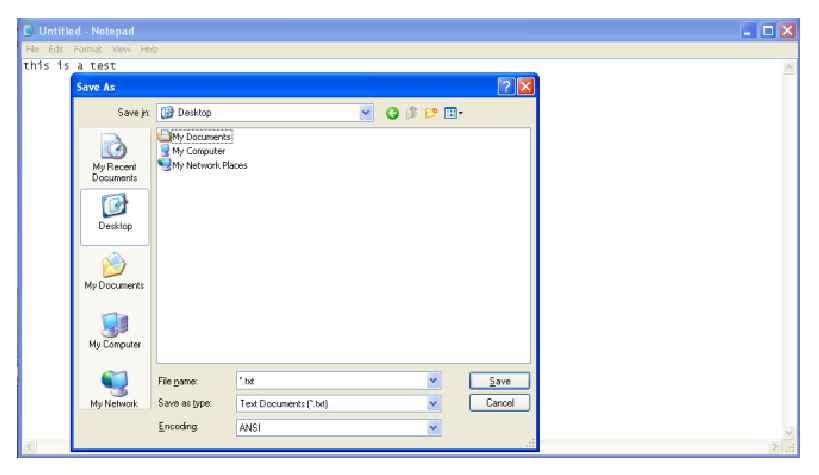
\includegraphics[width=65mm]{../en/figure17.eps}
\end{center}
\caption{Окно сохранения файла блокнота Windows.}\label{fig17}
\end{figure}

Открой снова консоль Питона и введи туда такие команды:

\begin{listing}
\begin{verbatim}
>>> f = open('c:\\test.txt')
>>> print(f.read())
\end{verbatim}
\end{listing}
\end{WINDOWS}

\begin{MAC}
	
Для этого давай откроем текстовый редактор (\includegraphics*[width=12mm]{../en/textedit-icon.eps}). Напечатай туда что-нибудь и сохрани на рабочий стол этот файл под именем «test.txt». Чтобы сохранить, нажми вверху (в меню) «Файл», потом выбери «Сохранить».

\begin{figure}
\begin{center}
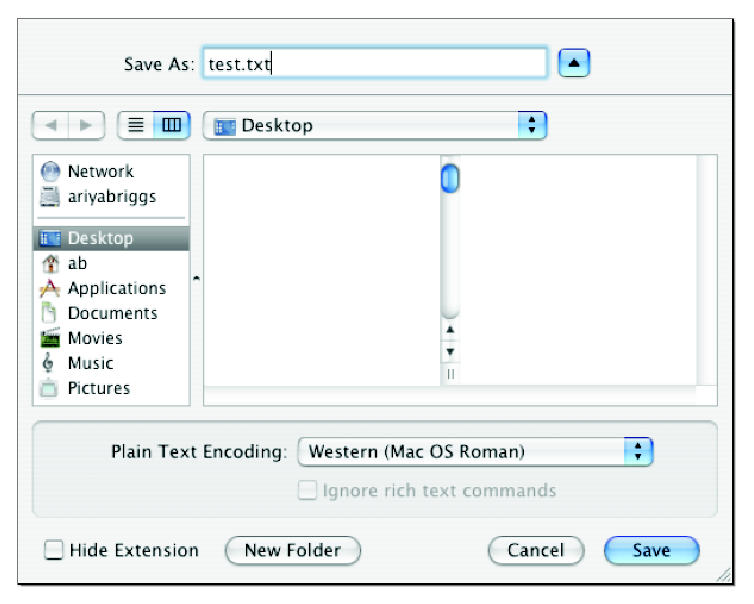
\includegraphics[width=65mm]{../en/figure18.eps}
\end{center}
\caption{Диалог сохранения файла в текстовом редакторе Mac OS X.}\label{fig18}
\end{figure}

Открой ещё раз консоль Питона и введи туда такие команды:

\begin{listing}
\begin{verbatim}
>>> f = open('Desktop/test.txt')
>>> print(f.read())
\end{verbatim}
\end{listing}
\end{MAC}

\begin{LINUX}
Для этого давай откроем текстовый редактор. Напечатай туда несколько слов и сохрани этот новый файл в свою домашнюю папку, нажав, например, кнопку «сохранить» где-то слева в верху экрана (твои родители должны были показать тебе, как сохранять, где-то в первой главе) и выбрав в качестве места для cохранения домашнюю папку. Назови файл «test.txt» (должно получиться, например, как на рисунке~\ref{fig19})
	
\begin{figure}
\begin{center}
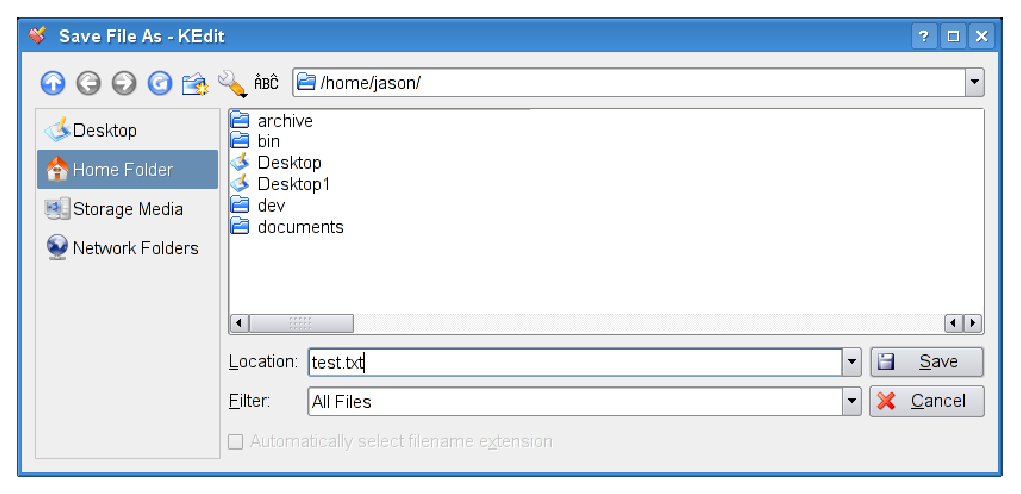
\includegraphics[width=65mm]{../en/figure19.eps}
\end{center}
\caption{Диалог сохранения может выглядеть, например, так}\label{fig19}
\end{figure}

Теперь снова открой питонью консоль и напечатай туда такие команды:

\begin{listing}
\begin{verbatim}
>>> f = open('test.txt')
>>> print(f.read())
\end{verbatim}
\end{listing}
\end{LINUX}

В консоли напечатается всё, что есть в файле.

Давай разберёмся, что этот кусочек кода делает. Первая строка вызывает функцию \code{open}, передавая ей имя файла в качестве параметра. Эта функция открывает файл, чтобы его потом использовать. Она возвращает специальное значение (объект), которое описывает этот файл. Потом у этого объекта можно вызывать функции, чтобы прочитать что-то из файла или записать в файл. Этот объект сохраняется в переменную \code{f} в нашей строчке кода.

Потом вторая строка вызывает у объекта \code{f} функцию \code{read} (используя точку после имени объекта: именно так вызываются функции у объектов), которая читает весь файл и возвращает результат как строку. Эта строка тут же и передаётся как параметр функции \code{print}, так что весь файл печатается в консоль.

\vspace{6pt}
\begin{center}
\fbox{\colorbox{PaleBlue}{\parbox{.75\linewidth} {
В приложении~\ref{app:builtinfunctions} (в конце книжки) написано ещё всякое разное про встроенные в Питон функции.
}}}
\end{center}

\section{Модули}\index{модули}

Ну что ж, с парой способов повторно использовать код мы уже познакомились. Во-первых, это функции, которые можно и самим создавать и вызывать, и использовать встроенные в Питон (\code{range}, \code{open}, \code{int}, \code{str}). Во-вторых, можно вызывать функции у объектов — про то, как их описывать, мы потом поговорим.

Ещё можно создавать модули: файлы, содержащие функции и объекты, сгруппированные вместе. Например, всё для работы со временем содержится в модуле \code{time}\index{модули!time}. Вот так мы говорим Питону, что будем в программе использовать функции и переменные из этого модуля:

\begin{listing}
\begin{verbatim}
>>> import time
\end{verbatim}
\end{listing}

Теперь мы можем обращаться к функциям из этого модуля, используя точку (точно так же, как к функциям какого-нибудь объекта):

\begin{listing}
\begin{verbatim}
>>> print(time.localtime())
(2006, 11, 10, 23, 49, 1, 4, 314, 1)
\end{verbatim}
\end{listing}

\code{localtime}\index{модули!time!localtime} — функция, которая возвращает текущие время и дату, сохранённые в кортеже (про кортежи было во второй главе раздел «Кортежи и списки», на странице \pageref{tuplesandlists}): год, месяц, день, час, минуту, секунду, номер дня недели, номер дня года и переведены ли часы на летнее время (1, если да; 0 — если нет). Можно воспользоваться ещё одной функцией из модуля \code{time}, чтобы превратить этот кортеж в более понятную строку:

\begin{listing}
\begin{verbatim}
>>> t = time.localtime()
>>> print(time.asctime(t))
'Sun Aug 30 21:40:59 2015'
\end{verbatim}
\end{listing}

Можно это сделать в одну строку:

\begin{listing}
\begin{verbatim}
>>> print(time.asctime(time.localtime()))
'Sun Aug 30 21:41:16 2015'
\end{verbatim}
\end{listing}

А можно и ещё чуть сократить:

\begin{listing}
\begin{verbatim}
>>> time.asctime()
'Sun Aug 30 21:41:44 2015'
\end{verbatim}
\end{listing}

Потому что функция \code{asctime} как раз печатает текущее время, если никаких параметров ей не передавать.

Может случиться так, что тебе нужно будет попросить того, кто пользуется твоей программой, ввести значение. Для этого можно напечатать эту просьбу на экране и потом считать то, что твоей программе в ответ напечатают. Функция, чтобы читать то, что вводят с клавиатуры, содержится в модуле \code{sys}:

\begin{listing}
\begin{verbatim}
import sys
\end{verbatim}
\end{listing}

В этом модуле есть объект \code{stdin}\index{модули!sys!stdin} (сокращение от английского «standard input», то есть «стандартный ввод»). А у этого объекта есть функция \code{readline} — считать строку текста, то есть всё, что напечатано до нажатия клавиши Enter. Клавиша Enter заканчивает строку (точно так же, как в любом текстовом редакторе). Можешь проверить, как эта функция работает, введя вот это в консоль:

\begin{listing}
\begin{verbatim}
>>> print(sys.stdin.readline())
\end{verbatim}
\end{listing}

Напечатай что-нибудь и нажми Enter. Питон ровно эту строку и напечатает.

Теперь можем вернуться к условному оператору \code{if} из четвёртой главы. Там был такой код:

\begin{listing}
\begin{verbatim}
>>> if age >= 10 and age <= 13:
...     print('Я знаю, тебе %s лет' % age)
... else:
...     print('Столько люди не живут.')
\end{verbatim}
\end{listing}

Вместо того чтобы заранее создавать и задавать значение переменной \code{age}, можно попросить кого-то ввести возраст с клавиатуры. Но сперва давай выделим этот код в функцию:

\begin{listing}
\begin{verbatim}
>>> def your_age(age):
...     if age >= 10 and age <= 13:
...         print('Я знаю, тебе %s лет' % age)
...     else:
...         print('Столько люди не живут.')
... 
\end{verbatim}
\end{listing}

Эту функцию можно вызвать, передав ей возраст как параметр. Прежде всего, давай убедимся, что функция работает как надо:

\begin{listing}
\begin{verbatim}
>>> your_age(20)
Столько люди не живут.
>>> your_age(10)
Я знаю, тебе 10 лет
\end{verbatim}
\end{listing}

Итак, мы теперь знаем, что проблем с функцией нет — давай сделаем так, чтобы она считывала с клавиатуры, сколько человеку лет:

\begin{listing}
\begin{verbatim}
>>> def your_age():
...     print('Сколько тебе лет? Введи число и нажми Enter: ')
...     age = int(sys.stdin.readline())
...     if age >= 10 and age <= 13:
...         print('Я знаю, тебе %s лет' % age)
...     else:
...         print('Столько люди не живут.')
... 
\end{verbatim}
\end{listing}

Тут в коде вызывается функция \code{int}. Этот потому что \code{readline} возвращает текст (строку, то есть), а нам результат надо сравнить с числами, то есть использовать как число (на странице \pageref{whatsthedifference} про это подробнее). Теперь можешь потестировать эту функцию: просто вызови её.

\begin{listing}
\begin{verbatim}
>>> your_age()
Сколько тебе лет? Введи число и нажми Enter:
10
Я знаю, тебе 10 лет
>>> your_age()
Сколько тебе лет? Введи число и нажми Enter:
15
Столько люди не живут.
\end{verbatim}
\end{listing}

\btw{Да, хотя ты печатаешь вроде как число, Питон считывает строку, состоящую из цифр, но не число. Нужно не забыть превратить эту строку в число функцией \code{int}.}

\vspace{6pt}
\fbox{\colorbox{PaleBlue}{\parbox{.75\linewidth} {
\code{sys} и \code{time} — всего лишь два из кучи модулей, которые устанавливаются вместе с Питоном. Ещё про некоторые (не про все) написано в конце книжки, в приложении \ref{app:afewpythonmodules}.
}}}

\section{Как ещё развлечься}

\btw{Итак, в этой главе мы изучили, как в Питоне повторно использовать код: для этого придумали функции и модули. Мы немного обсудили область видимости переменных: что переменные, объявленные вне функции, можно использовать изнутри неё (но изменения не будут видны снаружи), а переменные, объявленные в функции, только в ней и видны. Ещё мы научились создавать функции, используя инструкцию \code{def}}.

\subsection*{Упражнение 1}
В предыдущей главе во втором упражнении мы использовали цикл \code{for}, чтобы посчитать, сколько денег накопится на нашем банковском счёте за 10 лет, если положить туда 10 000 рублей. Было бы удобно прикинуть, сколько накопится денег при других условиях. Преврати код из того упражнения в функцию, которая принимает три параметра:

\begin{enumerate}
\item Сколько денег ты кладёшь в банк;
\item На сколько лет;
\item Сколько процентов годовых обещает банк.
\end{enumerate}

В результате эту функцию должно быть можно вызвать так, и она должна давать такие ответы:

\begin{listing}
\begin{verbatim}
>>> calculate_interest (1000, 1, 11)
1110.0
>>> calculate_interest (1200, 5, 13)
2210.922215159999
>>> calculate_interest (1500, 10, 15)
6068.33660356186
\end{verbatim}
\end{listing}

\subsection*{Упражнение 3}

Вместо того чтобы задавать значения параметров из программы, лучше сделать так, чтобы функция сама их спрашивала. Тогда тому, кто будет пользоваться этой программой, надо будет просто ввести значения с клавиатуры, а не менять программный код, передавая другие значения функции (можешь спросить, например, у мамы, что ей проще).

Используй функции \code{sys.stdin.readline} и \code{int}, чтобы считывать эти данные с клавиатуры внутри функции \code{calculate\_interest}. Функцию теперь можно вызывать вот так:

\begin{listing}
\begin{verbatim}
calculate_interest()
\end{verbatim}
\end{listing}

% !TeX encoding = UTF-8
% Use XeLaTeX to compile it
%
% Эта работа распространяется на условиях лицензии Creative Commons Attribution-Noncommercial-Share Alike 3.0 New Zealand License.
% Краткое описание лицензии есть тут: http://creativecommons.org/licenses/by-nc-sa/3.0/nz/deed.ru
% Полное — там же.
% Эту книгу можно невозбранно распространять и изменять, но только соблюдая следующие условия:
% сохраняя лицензию и не вводя дополнительных ограничений, бесплатно
% и указывая авторство как оригинальной части, так и изменённой.
% Автор оригинального английского текста — Jason R Briggs http://jasonrbriggs.com/
% Автор перевода — Егор Кочетов <Egor.Kochetoff@gmail.com>
%
% This work is licensed under the Creative Commons Attribution-Noncommercial-Share Alike 3.0 New Zealand License.
% To view a copy of this license, visit http://creativecommons.org/licenses/by-nc-sa/3.0/nz
% or send a letter to Creative Commons, 171 Second Street, Suite 300, San Francisco, California, 94105, USA.
%

\chapter{Коротенькая глава про файлы}\label{ch:ashortchapteraboutfiles}\index{функции!file}

Может статься, ты уже слышал, что такое файлы (тем более, что в прошлой главе мы их использовали). Но я на всякий случай расскажу.

Наверное, тебе доводилось сталкиваться с такими плоскими полиэтиленовыми папками для бумаг на кольцах — они обычно называются файлами. В них можно вкладывать какие-то записи на русском, английском, удмуртском языках (например) и ещё приклеивать на них наклейку с названием. И потом их можно складывать в большие картонные папки, чтобы все эти файлики лежали рядом.

В компьютере всё примерно так же, только файлов можно создавать из ничего сколько угодно (ну… почти, пока место в компьютере не кончится). И у каждого файла всегда обязательно есть название. В файле может быть записано что угодно любой программой — мы, например, записывали в файлы текст простым текстовым редактором в предыдущих главах. И потом файл можно открыть любой программой — главное, чтобы программа, которая открывает файл, понимала тот «язык» (он называется «формат»), которым пользовалась программа, которая создавала файл. Файлы в компьютере можно складывать в папки, или директории\footnote{На самом деле, директория — тоже файл: в нём просто перечислен список, какие именно файлы лежат внутри.}. Если аккуратно разложить все файлы в компьютере по папкам, то в них существенно проще ориентироваться, чем если они лежат кучей в одной папке или в беспорядке в разных папках.

Мы уже использовали объект, описывающий файл в Питоне, в предыдущей главе, таким образом:

\begin{WINDOWS}

\begin{listing}
\begin{verbatim}
>>> f = open('c:\\test.txt')
>>> print(f.read())
\end{verbatim}
\end{listing}

\end{WINDOWS}

\begin{MAC}

\begin{listing}
\begin{verbatim}
>>> f = open('Desktop/test.txt')
>>> print(f.read())
\end{verbatim}
\end{listing}

\end{MAC}

\begin{LINUX}

\begin{listing}
\begin{verbatim}
>>> f = open('test.txt')
>>> print(f.read())
\end{verbatim}
\end{listing}
 

Так мы открываем для чтения файл «test.txt». Файл при этом находится в \emph{текущей папке}. Когда ты запускаешь Питон из консоли, то текущая папка остаётся той, которая была. Если ты не делал специальных манипуляций, то это просто домашняя папка. Если бы тебе хотелось напечатать файл «письмо.txt», который лежит в папке «почта», то надо было бы написать так:
\begin{listing}
\begin{verbatim}
>>> f = open ('почта/письмо.txt')
>>> print(f.read())
\end{verbatim}
\end{listing}

\end{LINUX}

Файловый объект (он же объект типа \code{file}) не ограничивается только функцией \code{read}. В конце концов, если бы в папку с документами нельзя было добавить новых, мало пользы было бы от такой папки.

Мы можем создать новый пустой файл, передав ещё один параметр функции \code{open}, вот так:

\begin{listing}
\begin{verbatim}
>>> f = open('myfile.txt', 'w')
\end{verbatim}
\end{listing}

Параметр «w» — сокращение от английского «write» — записать. Так мы Питону говорим, что нам из этого файла не надо ничего читать, надо только записывать. Поэтому если файл с таким именем уже есть, то он будет тут же очищен, а если его нет — то будет создан новый пустой.

Можем что-нибудь записать в этот файл:

\begin{listing}
\begin{verbatim}
>>> f = open('myfile.txt', 'w')
>>> f.write('что-нибудь')
\end{verbatim}
\end{listing}

Теперь надо сказать Питону закрыть файл. Потому что к этому моменту он запомнил, что надо будет записать в файл \code{f} всё, что мы попросили, но ещё не записывал. Запоминать быстро, а записывать в файл — долго. По-настоящему Питон запишет в файл, только если программа завершится (то есть если закрыть консоль Питона, в которой мы открыли файл); или если помнить придётся слишком много — тогда какую-то часть Питон запишет в файл, а остальную будет всё ещё держать в уме; или если явно попросить Питон записать в файл всё, что нужно — например, функцией \code{close}:

\begin{listing}
\begin{verbatim}
>>> f = open('myfile.txt', 'w')
>>> f.write('что-нибудь')
>>> f.close()
\end{verbatim}
\end{listing}

Можешь теперь этот файл открыть текстовым редактором и прочитать там записанный текст. Можно, опять-таки, воспользоваться Питоном для чтения текста:

\begin{listing}
\begin{verbatim}
>>> f = open('myfile.txt')
>>> print(f.read())
this is a test file
\end{verbatim}
\end{listing}

Может показаться странным, зачем все эти хитрости с запоминанием и записыванием только потом. Простой ответ — чтобы было быстрее.

Дело в том, что записывать в файл может быть в тысячу раз медленнее, чем запоминать (в \emph{оперативную память}). Чтобы хоть как-то это исправить, в файл пишут сразу большой кусочек данных за раз, так получается быстрее. Всё, что меньше, чем размер кусочка, Питон держит в памяти. Ещё бывает, что нужно что-то записать в файл, потом в другом месте программы это прочитать из файла, а потом файл и вовсе удалить за ненадобностью. Так вот если данных немного, то их можно и совсем не записывать в файл, а только запомнить, что сильно ускоряет работу программы. Вообще, подобным образом с файлами обращается не только Питон, но и большинство программ.

\newpage
% !TeX encoding = UTF-8
% Use XeLaTeX to compile it
%
% Эта работа распространяется на условиях лицензии Creative Commons Attribution-Noncommercial-Share Alike 3.0 New Zealand License.
% Краткое описание лицензии есть тут: http://creativecommons.org/licenses/by-nc-sa/3.0/nz/deed.ru
% Полное — там же.
% Эту книгу можно невозбранно распространять и изменять, но только соблюдая следующие условия:
% сохраняя лицензию и не вводя дополнительных ограничений, бесплатно
% и указывая авторство как оригинальной части, так и изменённой.
% Автор оригинального английского текста — Jason R Briggs http://jasonrbriggs.com/
% Автор перевода — Егор Кочетов <Egor.Kochetoff@gmail.com>
%
% This work is licensed under the Creative Commons Attribution-Noncommercial-Share Alike 3.0 New Zealand License.
% To view a copy of this license, visit http://creativecommons.org/licenses/by-nc-sa/3.0/nz
% or send a letter to Creative Commons, 171 Second Street, Suite 300, San Francisco, California, 94105, USA.
%

\chapter{Черепаховое изобилие}\index{turtle!подробнее}\label{ch:turtlesgalore}

Пришло время вернуться к черепахе из модуля \code{turtle}, о которой мы говорили в главе \ref{ch:turtles}. Чтобы создать холст, на котором бы рисовала черепаха, мы использовали вот такой код:

\begin{listing}
\begin{verbatim}
>>> import turtle
>>> t = turtle.Pen()
\end{verbatim}
\end{listing}

Раньше, когда мы не знали про циклы (\code{for} и \code{while}) и условный оператор (\code{if}), мы использовали самые простые функции для рисования. Вот так мы рисовали квадрат:

\begin{listing}
\begin{verbatim}
>>> t.forward(50)
>>> t.left(90)
>>> t.forward(50)
>>> t.left(90)
>>> t.forward(50)
>>> t.left(90)
\end{verbatim}
\end{listing} 

Этот же код можно здорово сократить, если использовать цикл:

\begin{listing}
\begin{verbatim}
>>> t.reset()
>>> for x in range(1,5):
...     t.forward(50)
...     t.left(90)
...
\end{verbatim}
\end{listing}

Так куда меньше нужно набирать. К тому же, если читать этот код, то гораздо быстрее можно понять, что тут черепашка четыре раза идёт вперёд и поворачивает налево. Без цикла это не так сразу ясно.

Используя цикл, можно довольно просто изменить код так, чтобы рисовалась какая-нибудь фигура похитрее. Например, попробуй запустить вот этот код:

\begin{listing}
\begin{verbatim}
>>> t.reset()
>>> for x in range(1,9):
...     t.forward(100)
...     t.left(225)
...
\end{verbatim}
\end{listing}

Он рисует восьмиконечную звезду, как на картинке \ref{fig20}. Каждый раз, когда черепашка проходит 100 пикселей, она поворачивает влево на 225 градусов.

\begin{figure}
\begin{center}
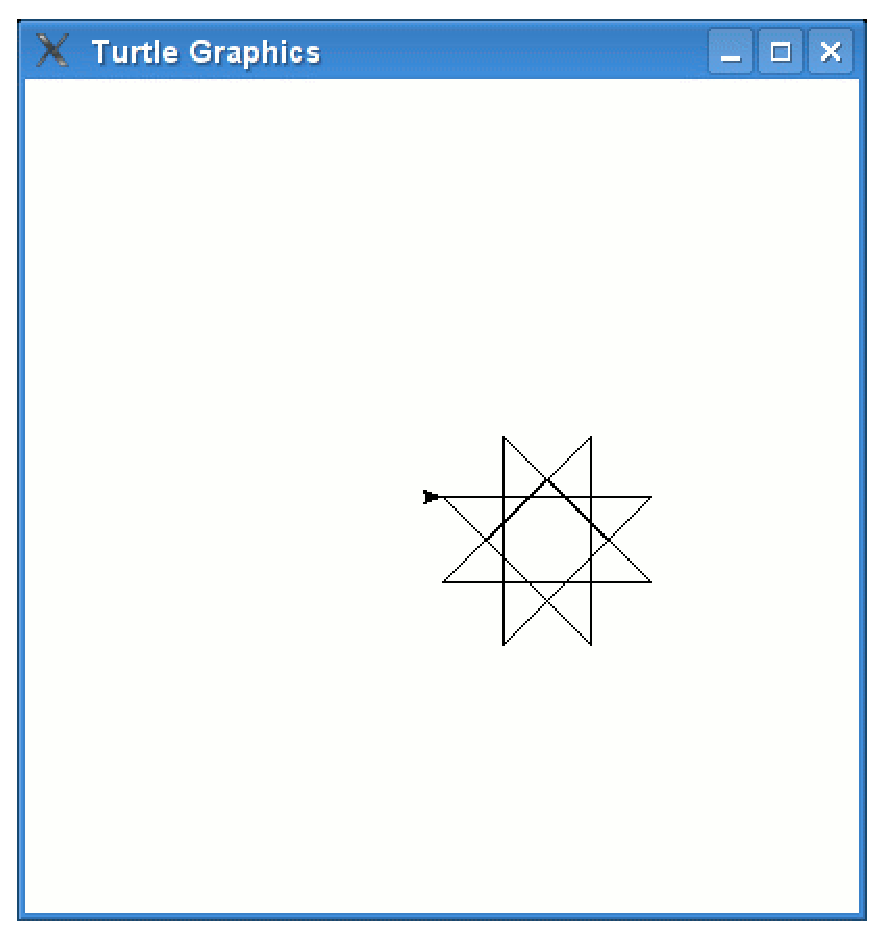
\includegraphics[width=72mm]{../en/figure20.eps}
\end{center}
\caption{Восьмиконечная звезда в исполнении черепашки.}\label{fig20}
\end{figure}

Если ещё немного поменять угол (до 175 градусов) и сделать длиннее цикл (37 шагов), то можно нарисовать звезду, у которой будет ещё больше лучей (как на картинке \ref{fig21}):

\begin{listing}
\begin{verbatim}
>>> t.reset()
>>> for x in range(1,38):
...     t.forward(100)
...     t.left(175)
...
\end{verbatim}
\end{listing}

\begin{figure}
\begin{center}
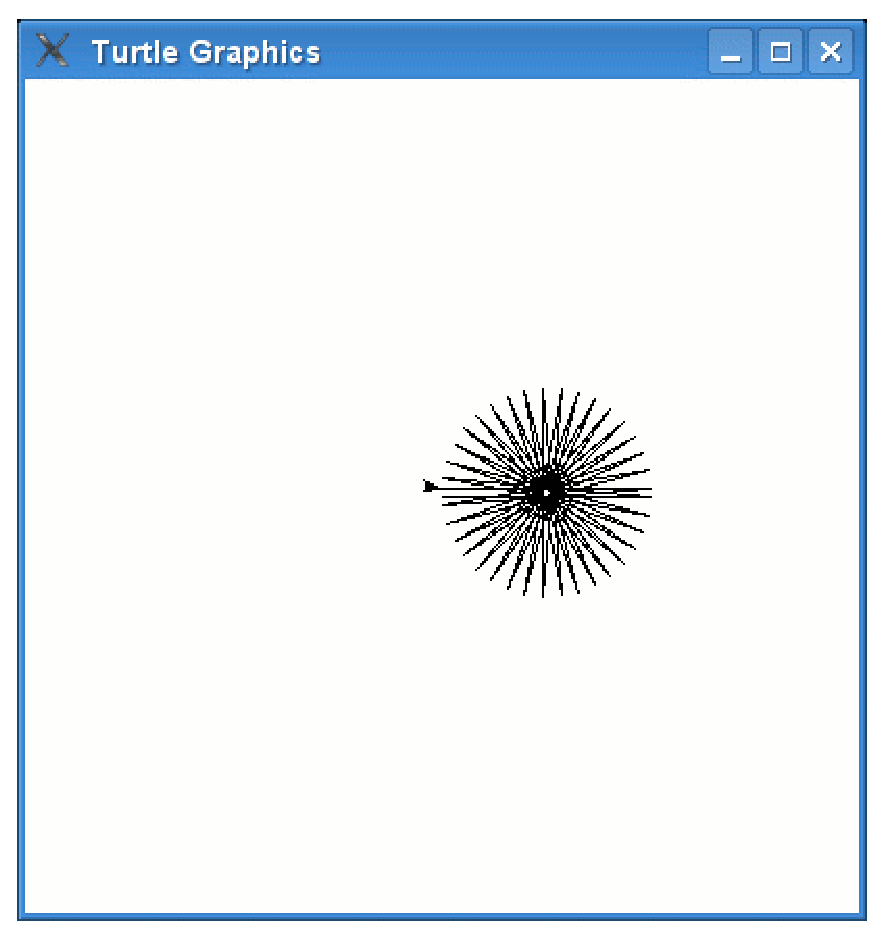
\includegraphics[width=72mm]{../en/figure21.eps}
\end{center}
\caption{Звезда, у которой много лучей.}\label{fig21}
\end{figure}

Или вот можно нарисовать что-то среднее между звездой и спиралью, как на рисунке \ref{fig22}:

\begin{listing}
\begin{verbatim}
>>> for x in range(1,20):
...     t.forward(100)
...     t.left(95)
...
\end{verbatim}
\end{listing}

\begin{figure}
\begin{center}
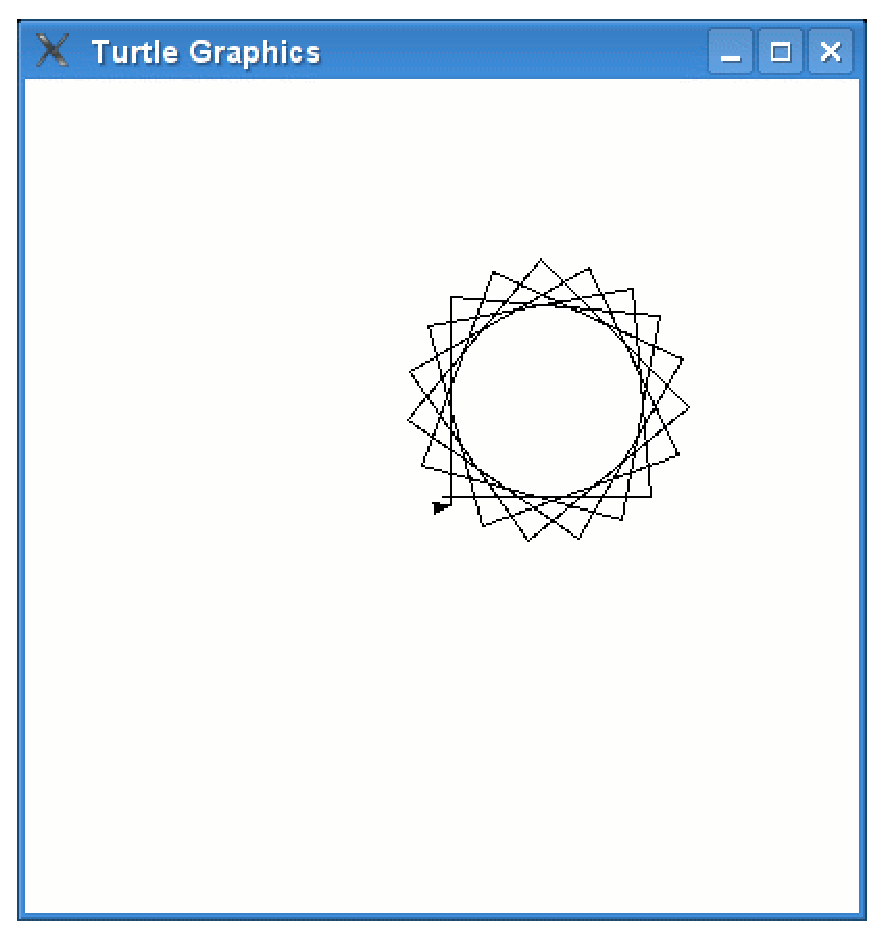
\includegraphics[width=72mm]{../en/figure22.eps}
\end{center}
\caption{Звезда с кучей лучей.}\label{fig22}
\end{figure}

Давай теперь попробуем нарисовать что-нибудь, что рисовать сложнее. Например, вот так:

\begin{listing}
\begin{verbatim}
>>> t.reset()
>>> for x in range(1,19):
...     t.forward(100)
...     if x % 2 == 0:
...         t.left(175)
...     else:
...         t.left(225)
...
\end{verbatim}
\end{listing}

В этом коде мы проверяем, содержится ли в переменной \code{x} чётное число. Для этого нам пригодится операция «\code{\%}», то есть получение остатка от деления: число ведь нечётное, если делится на два с остатком, и чётное — если без, то есть если остаток равен 0. Говоря по-питоньи, \code{if (x \% 2 == 0)}, то \code{x} — чётное число.

Если запустить код, который написан выше, то получится звезда с девятью лучами, как на рисунке \ref{fig23}.

\begin{figure}
\begin{center}
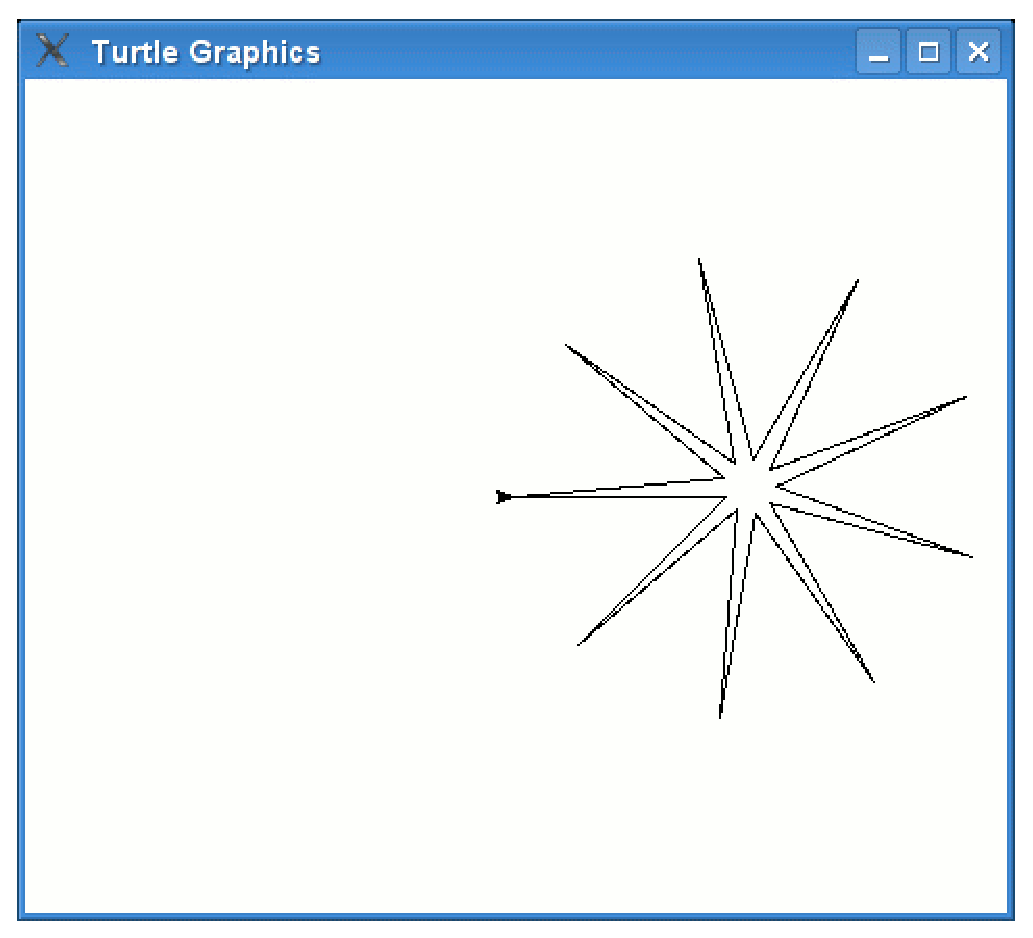
\includegraphics[width=84mm]{../en/figure23.eps}
\end{center}
\caption{Звезда с девятью лучами.}\label{fig23}
\end{figure}

Умение черепашки рисовать не ограничивается просто чёрно-белыми линиями и способностью начинать и заканчивать рисовать. Можно делать и цветные картинки, например такие:

\begin{listing}
\begin{verbatim}
t.color(1,0,0)
t.begin_fill()
t.forward(100)
t.left(90)
t.forward(20)
t.left(90)
t.forward(20)
t.right(90)
t.forward(20)
t.left(90)
t.forward(60)
t.left(90)
t.forward(20)
t.right(90)
t.forward(20)
t.left(90)
t.forward(20)
t.end_fill()
t.color(0,0,0)
t.up()
t.forward(10)
t.down()
t.begin_fill()
t.circle(10)
t.end_fill()
t.setheading(0)
t.up()
t.forward(90)
t.right(90)
t.forward(10)
t.setheading(0)
t.begin_fill()
t.down()
t.circle(10)
t.end_fill()
\end{verbatim}
\end{listing}

Код выше — долгий-долгий, утомительный и бессмысленный способ нарисовать что-то вроде машинки (она на картинке \ref{fig24}). Этот код ценен не машинкой. Он показывает, какие ещё функции есть у черепашки: \code{color} — меняет цвет фломастера, которым черепашка рисует; \code{fill} — закрашивает область на холсте всю одним цветом; \code{circle} — рисует кружочек заданного размера (диаметра).

\begin{figure}
\begin{center}
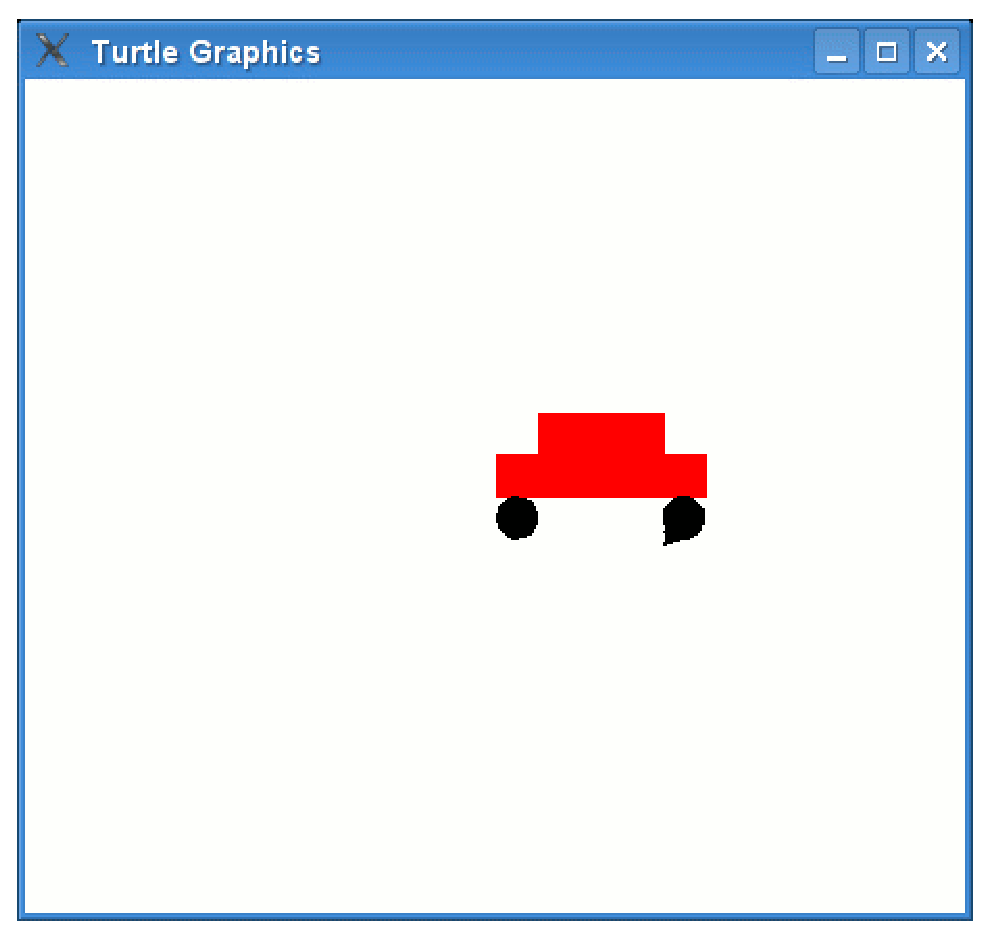
\includegraphics[width=80mm]{../en/figure24.eps}
\end{center}
\caption{Не стоит пытаться рисовать машину черепахой!}\label{fig24}
\end{figure}

\section{Добавим цвета}

Функция \code{color}\index{черепашка!color} принимает 3 параметра. Первый — интенсивность красного цвета, второй — зелёного, третий — синего.

\emph{Почему красный зелёный и синий? И что это за интенсивность такая?}

Если тебе доводилось смешивать краски, то ты можешь уже догадываться, как черепашка (и вообще, любая программа, рисующая на экране компьютера) получает цвета. Если ты смешаешь краски двух цветов, то получишь третий цвет, которым можно что-нибудь нарисовать\footnote{Когда рисуешь красками, то нужно чтобы были красный, жёлтый и синий цвета, из них можно получить любой другой. Компьютеру нужны красный, зелёный и синий, потому что на экране он рисует не красками, а наоборот, светом.}. Если смешать синюю и красную краски, то получится сиреневая, а если намешать слишком много красок, то может получиться серо-буро-малиновый цвет или просто какая-то коричневая грязька. В компьютере можно так же смешивать цвета: если взять одинаковое количество красного и зелёного, например, то получится жёлтый. Но в компьютере мы смешиваем цвета, которыми светит сам экран, а не цвета краски, которой мы рисуем по бумаге.

Давай на секундочку вернёмся к смешиванию краски. Представь, что у нас есть три чашки с краской. Одна чашка с красной, другая — с зелёной и третья — с синей. Каждая чашка полна краски до краёв. Теперь если мы хотим взять целую чашку краски для получения цвета, мы должны для этого цвета передать черепашке значение 1 (то есть 100\%). Если краску из этой чашки мы брать не хотим — то значение 0. Если хотим взять полчашки, например — то 0.5 (то есть ½). Если взять целую чашку красной и зелёной краски, то в результате получится жёлтая. Давай нарисуем жёлтый круг:

\begin{listing}
\begin{verbatim}
>>> t.color(1,1,0)
>>> t.begin_fill()
>>> t.circle(50)
>>> t.end_fill()
\end{verbatim}
\end{listing}

Тут мы вызываем функцию \code{color}, передавая ей значение 1 (100\%) для красного и зелёного цвета и 0 — для синего. Давай для дальнейших экспериментов с цветом заведём функцию, которая будет нам рисовать тем цветом, которым мы попросим:

\begin{listing}
\begin{verbatim}
>>> def draw_circle(red, green, blue):
...     t.color(red, green, blue)
...     t.begin_fill()
...     t.circle(50)
...     t.end_fill()
...
\end{verbatim}
\end{listing}

Можем нарисовать ярко-зелёный круг, взяв целую чашку зелёной краски.

\begin{listing}
\begin{verbatim}
>>> draw_circle(0, 1, 0)
\end{verbatim}
\end{listing}

А можем взять только полчашки зелёной краски…

\begin{listing}
\begin{verbatim}
>>> draw_circle(0, 0.5, 0)
\end{verbatim}
\end{listing}

…и круг получится тёмно-зелёным. Это может показаться странным: сколько краски ни возьми в реальном мире, круг всё равно будет одинаково зелёным. Но хитрость в том, что на самом деле нет. Если нарисовать тот же круг на белой бумаге, взяв мало краски, то сквозь круг будет просвечивать белая бумага, и круг будет белее, чем цвет самой краски. А компьютер, наоборот, рисует светом на чёрном экране. Мы сказали ему взять 0.5 чашки краски, то есть «половинное количество краски», и круг стал темнее, как будто сквозь него просвечивает чёрный экран.

Можешь понаблюдать за таким же эффектом, если рисовать синим и красным цветом: круг будет ярче и светлее, если «брать целую чашку краски», то есть передавать 1 в качестве значения интенсивности цвета:

\begin{listing}
\begin{verbatim}
>>> draw_circle(1, 0, 0)
>>> draw_circle(0.5, 0, 0)

>>> draw_circle(0, 0, 1)
>>> draw_circle(0, 0, 0.5)
\end{verbatim}
\end{listing}

Используя разные сочетания красного, зелёного и синего цветов, можно получить очень много цветов, почти все, которые человек может различить. Например, если смешать 100\% красного света, 85\% зелёного и не брать синего, то получится золотистый свет:
\begin{listing}
\begin{verbatim}
>>> draw_circle(1, 0.85, 0)
\end{verbatim}
\end{listing}

А малиновый можно получить, взяв 100\% красного, 70\% зелёного и 75\% синего:

\begin{listing}
\begin{verbatim}
>>> draw_circle(1, 0.70, 0.75)
\end{verbatim}
\end{listing}

Оранжевый — взяв 100\% красного и 65\% зелёного; коричневый — 60\% красного, 30\% зелёного и 15\% синего:

\begin{listing}
\begin{verbatim}
>>> draw_circle(1, 0.65, 0)
>>> draw_circle(0.6, 0.3, 0.15)
\end{verbatim}
\end{listing}

И я просто напомню, что всегда можно очистить холст, написав \code{t.clear()}.

\section{Темнота}\index{turtle!color!чёрный}

Ты же знаешь, что произойдёт если ночью выключить весь свет? Всё станет чёрным.

Так и в компьютере происходит. Если не брать никакого света для рисования, то рисунок будет чёрным (цвета выключенного монитора):

\begin{listing}
\begin{verbatim}
>>> draw_circle(0, 0, 0)
\end{verbatim}
\end{listing}

Этот код рисует чёрный круг, как на картинке \ref{fig25}.

\begin{figure}
\begin{center}
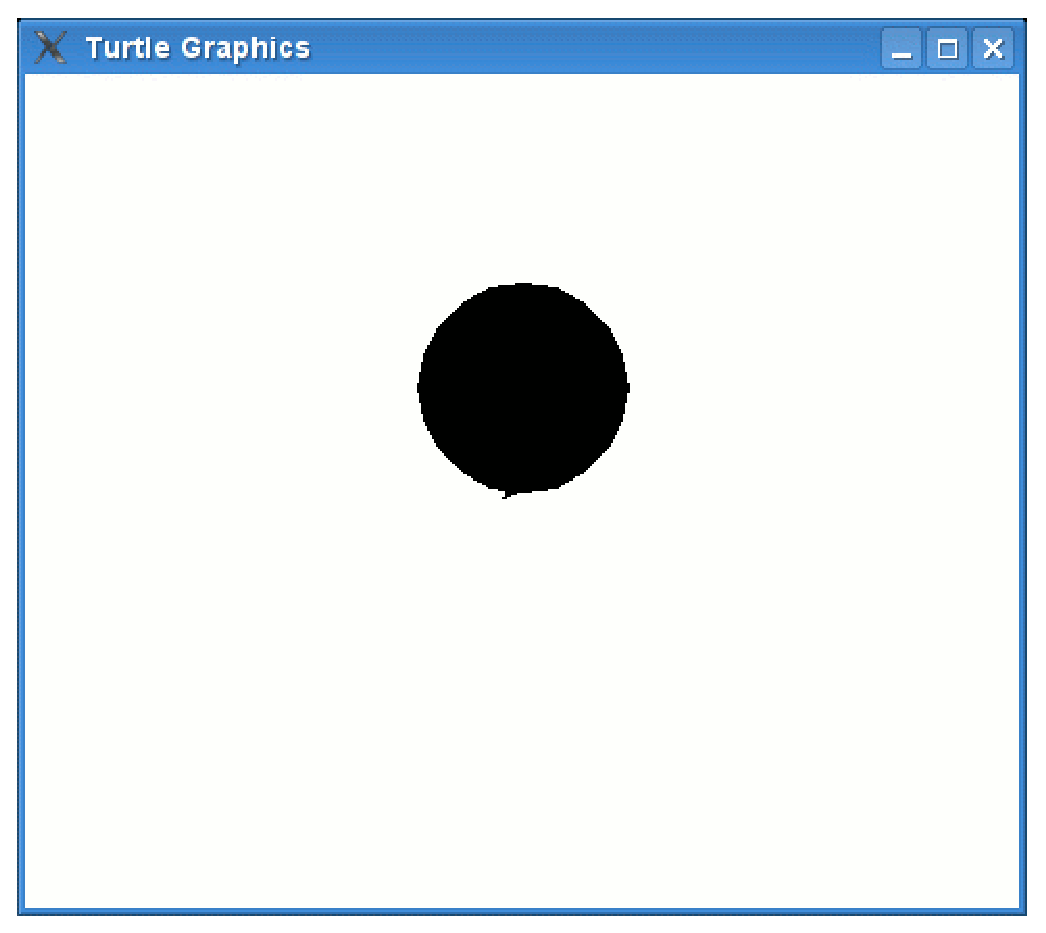
\includegraphics[width=85mm]{../en/figure25.eps}
\end{center}
\caption{Чёрная дыра!}\label{fig25}
\end{figure}

А если взять для рисования весь свет, то есть 100\% красного, 100\% зелёного и 100\% синего, то получится белый. Вот этот код уберёт обратно в небытие чёрный кружок (закрасит его белым):

\begin{listing}
\begin{verbatim}
>>> draw_circle(1,1,1)
\end{verbatim}
\end{listing}

\section{Закрашиваем рисунки}\index{черепашка!fill}

Возможно, ты уже догадался, что функция \code {begin\_fill} включает заливку цветом, а \code{end\_fill} — выключает. На самом деле, именно в момент выключения Питон и заливает нужную часть рисунка, а до тех пор только запоминает, куда потом лить краску. Зная это, мы можем нарисовать закрашенный квадрат. Вот код, который рисует просто квадрат:

\begin{listing}
\begin{verbatim}
>>> t.forward(50)
>>> t.left(90)
>>> t.forward(50)
>>> t.left(90)
>>> t.forward(50)
>>> t.left(90)
>>> t.forward(50)
>>> t.left(90)
\end{verbatim}
\end{listing}

Чтобы было проще рисовать много квадратов, да ещё и разного размера, завернём этот код в функцию:

\begin{listing}
\begin{verbatim}
>>> def mysquare(size):
...     t.forward(size)
...     t.left(90)
...     t.forward(size)
...     t.left(90)
...     t.forward(size)
...     t.left(90)
...     t.forward(size)
...     t.left(90)
\end{verbatim}
\end{listing}

Всё ли вышло успешно? Давай проверим.

\begin{listing}
\begin{verbatim}
>>> mysquare(50)
\end{verbatim}
\end{listing}

У меня квадрат нарисовался.

\emph {…в воображении. В книге нет консоли питона, но даже у книги есть воображение.}

Если присмотреться к этому коду, можно заметить, что в нём кучу раз повторяются одни и те же две строки. А если ещё пристальнее присмотреться, то даже удастся сосчитать, сколько раз они повторяются: четыре. Так что тут хорошо бы смотрелся цикл — вот такой:

\begin{listing}
\begin{verbatim}
>>> def mysquare(size):
...     for x in range(0,4):
...         t.forward(size)
...         t.left(90)
\end{verbatim}
\end{listing}

Так гораздо короче писать, меньше читать, и быстрее можно понять, что происходит. Можешь попробовать нарисовать квадратов всякого разного размера:

\begin{listing}
\begin{verbatim}
>>> t.reset()
>>> mysquare(25)
>>> mysquare(50)
>>> mysquare(75)
>>> mysquare(100)
>>> mysquare(125)
\end{verbatim}
\end{listing}

Должно получиться что-то вроде рисунка \ref{fig26}.

\begin{figure}
\begin{center}
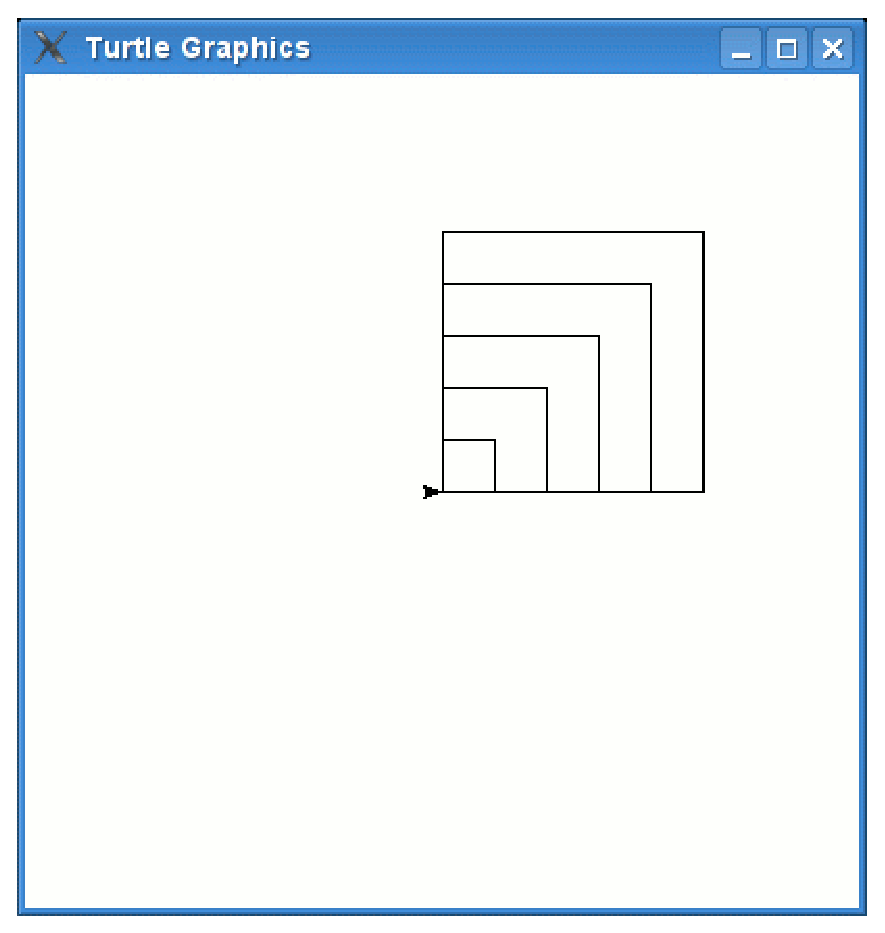
\includegraphics[width=72mm]{../en/figure26.eps}
\end{center}
\caption{Квадратики. Много.}\label{fig26}
\end{figure}

Ну а теперь можно приступить к рисованию закрашенных квадратов. Прежде всего, надо очистить холст от тех шедевров, что на нём уже есть:

\begin{listing}
\begin{verbatim}
>>> t.reset()
\end{verbatim}
\end{listing}

Потом включить заливку и нарисовать квадрат:

\begin{listing}
\begin{verbatim}
>>> t.begin_fill()
>>> mysquare(50)
\end{verbatim}
\end{listing}

…и потом наконец закрасить нарисованное:

\begin{listing}
\begin{verbatim}
>>> t.end_fill()
\end{verbatim}
\end{listing}

В результате получается картинка \ref{fig27}.

\begin{figure}
\begin{center}
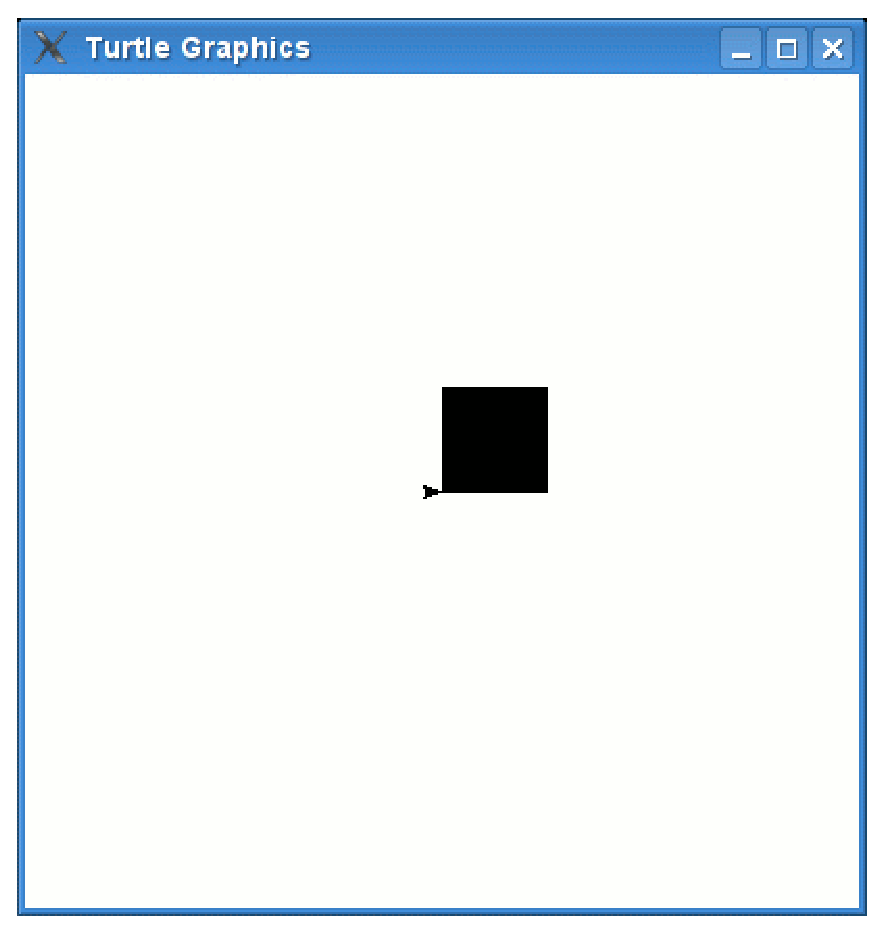
\includegraphics[width=72mm]{../en/figure27.eps}
\end{center}
\caption{Чёрный квадрат.}\label{fig27}
\end{figure}

Можно сделать рисование закрашенных квадратов чуточку удобнее: добавить в функцию рисования квадрата параметр, в зависимости от которого квадрат будет получаться или закрашенным, или нет:

\begin{listing}
\begin{verbatim}
>>> def mysquare(size, filled):
...    if filled == True:
...        t.begin_fill()
...    for x in range(0,4):
...        t.forward(size)
...        t.left(90)
...    if filled == True:
...        t.end_fill()
...
\end{verbatim}
\end{listing}

Первые две строка проверяют, равна ли переменная \code{filled} «истине» (\code{True} по-английски), то есть просили ли нас закрашивать. Если да, то включается заливка цветом. Потом рисуется кварат, потом заливка завершается, если нас вообще просили закрашивать. Теперь закрашенный квадрат можно нарисовать так:
\begin{listing}
\begin{verbatim}
>>> mysquare(50, True)
\end{verbatim}
\end{listing}

…а не закрашенный — вот так:

\begin{listing}
\begin{verbatim}
>>> mysquare(150, False)
\end{verbatim}
\end{listing}

И результат получается, как на рисунке \ref{fig28}… мне он напоминает безумный квадратный глаз.

\begin{figure}
\begin{center}
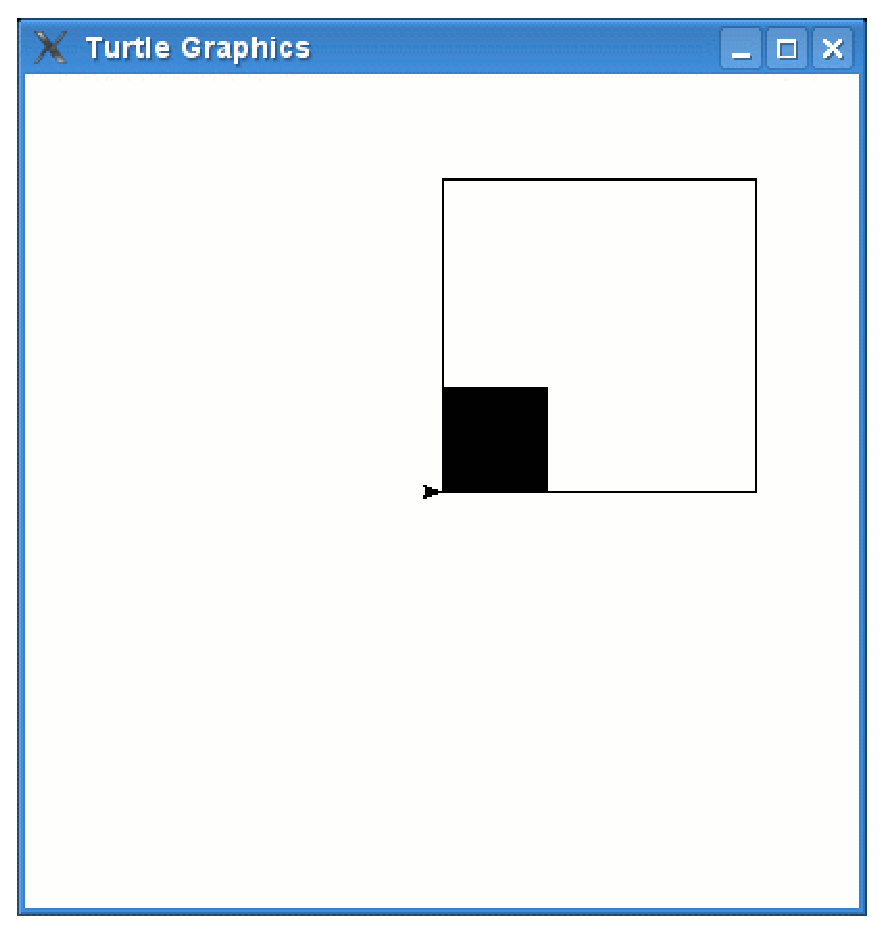
\includegraphics[width=72mm]{../en/figure28.eps}
\end{center}
\caption{Квадратный глаз}\label{fig28}
\end{figure}

Примерно так можно рисовать и всё остальное, что в голову взбредёт, и закрашивать цветом. Например, можем сделать функцию рисования звезды, которую мы в начале главы рисовали:

\begin{listing}
\begin{verbatim}
>>> for x in range(1,19):
...     t.forward(100)
...     if x % 2 == 0:
...         t.left(175)
...     else:
...         t.left(225)
...
\end{verbatim}
\end{listing}

Заворачиваем это в функцию, добавляем параметр, указывающий, надо ли закрашивать звезду (и ещё размер добавим, как для квадрата тоже), и получаем такой код:

\begin{listing}
\begin{verbatim}
1.  >>> def mystar(size, filled):
2.  ...     if filled:
3.  ...         t.begin_fill()
4.  ...     for x in range(1,19):
5.  ...         t.forward(size)
6.  ...         if x % 2 == 0:
7.  ...             t.left(175)
8.  ...         else:
9.  ...             t.left(225)
10. ...     if filled:
11. ...         t.end_fill()
\end{verbatim}
\end{listing}

Давай теперь проверим, что эта функция на самом деле делает: попробуем нарисовать золотистую звезду:

\begin{listing}
\begin{verbatim}
>>> t.color(1, 0.85, 0)
>>> mystar(120, True)
\end{verbatim}
\end{listing}

Черепашка должна изобразить рисунок \ref{fig29}. Теперь давай добавим к этой звезде чёрный контур: поменяем цвет, выключим заливку и нарисуем звезду того же размера ещё раз:

\begin{figure}
\begin{center}
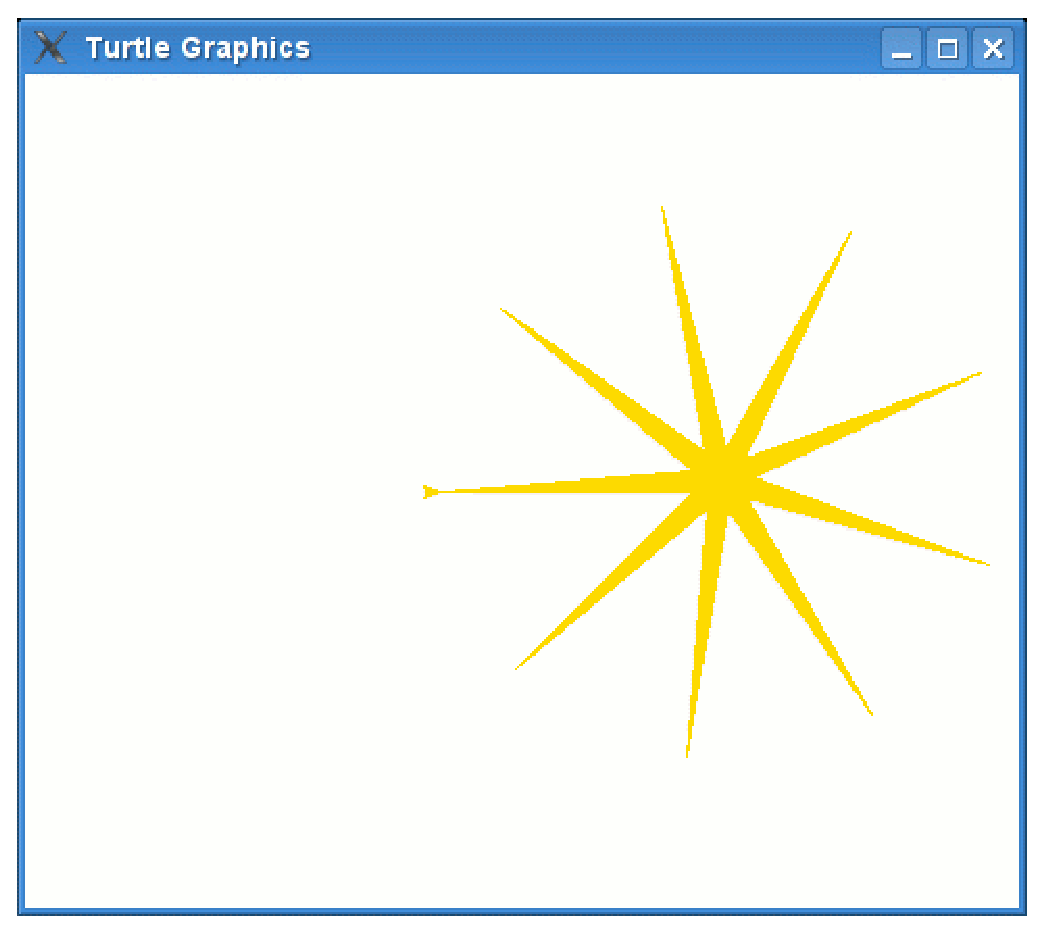
\includegraphics[width=85mm]{../en/figure29.eps}
\end{center}
\caption{Золотая звезда.}\label{fig29}
\end{figure}

\begin{listing}
\begin{verbatim}
>>> t.color(0,0,0)
>>> mystar(120, False)
\end{verbatim}
\end{listing}

Теперь звезда должна выглядеть так: \ref{fig30}.

\begin{figure}
\begin{center}
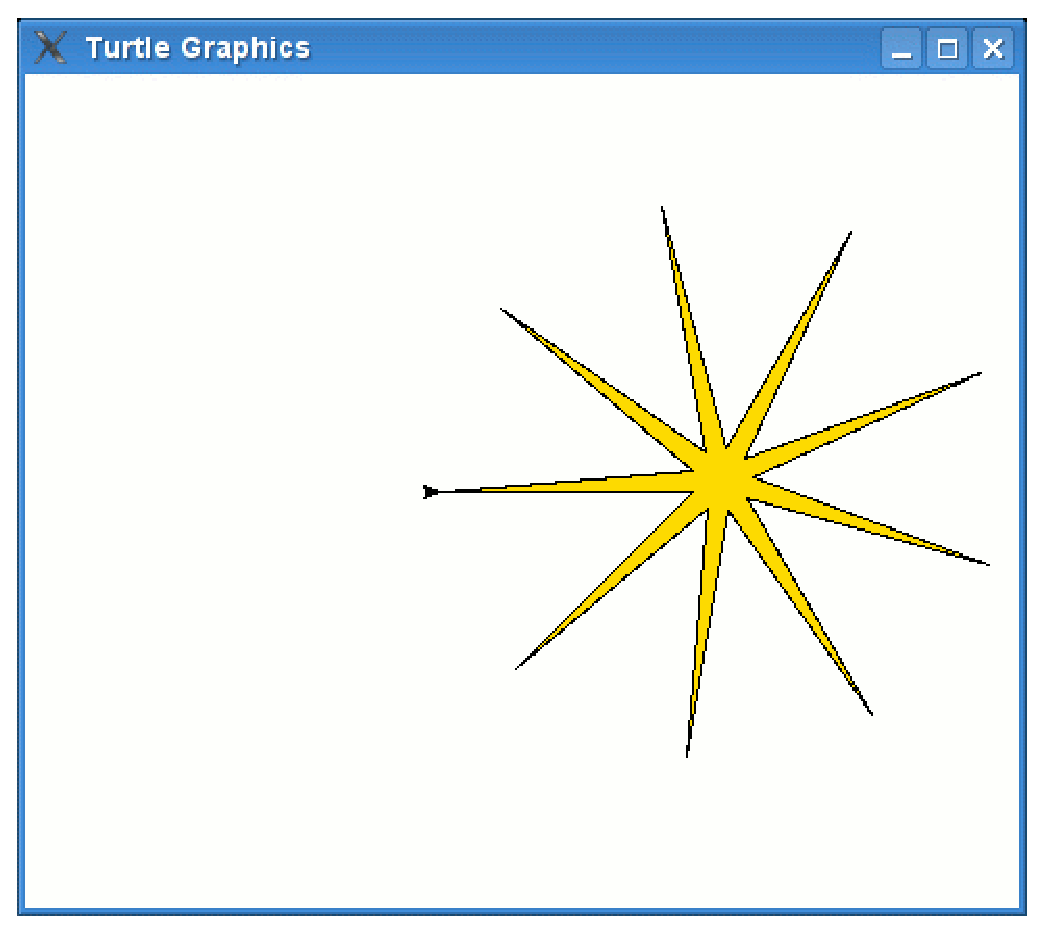
\includegraphics[width=85mm]{../en/figure30.eps}
\end{center}
\caption{Звёздочка с контуром.}\label{fig30}
\end{figure}

\section{Как ещё развлечься}

\emph{В этой главе мы посмотрели на разные функции черепашки — модуля turtle Питона — и с её помощью нарисовали разные геометрические фигуры. Мы создали функции для рисования фигур, а также для закраски их цветом.}

\subsection*{Упражнение 1}
Ну хорошо, вот мы нарисовали звёздочки, квадратики, прямоугольники. А как насчёт восьмиугольника? Попробуй нарисовать его. (Поворачивай на 45 градусов, это ключ к успеху).

\subsection*{Упражнение 2}
Создай функцию для рисования закрашенных и не закрашенных восьмиугольников разного размера.

\newpage


\printindex
\end{document}
